\باب{فوریئر تجزیہ}

\حصہ{تکونیاتی فوریئر تسلسل}
\اصطلاح{دوری تفاعل}\فرہنگ{دوری!تفاعل}\فرہنگ{تفاعل!دوری}\حاشیہب{periodic function}\فرہنگ{periodic!function} سے مراد وہ تفاعل ہے جو درج ذیل مساوات پر پورا اترتا ہے جہاں \عددی{T_0}  \اصطلاح{دوری عرصہ}\فرہنگ{دوری عرصہ}\حاشیہب{time period}\فرہنگ{time period} کہلاتی ہے۔
\begin{align}
f(t)=f(t+nT_0), \quad n=\mp 1, \mp 2, \mp3, \cdots
\end{align}
درج بالا مساوات کہتی ہے کہ  کسی بھی لمحہ \عددی{t} پر دوری تفاعل کی قیمت \عددی{f(t)} اور اس لمحے سے \عددی{T_0} وقت بعد تفاعل کی قیمت \عددی{f(t+T_0)} برابر ہیں۔شکل \حوالہ{شکل_فوریئر_دوری_عرصہ} میں اس کی وضاحت  کی گئی ہے۔
\begin{figure}
\centering
\begin{tikzpicture}
\begin{axis}[kStyleCircuitsA,xtick={115,475},xticklabels={$t$,$t+T_0$},ytick=\empty]
\pgfmathsetmacro{\kt}{115}
\pgfmathsetmacro{\ktt}{\kt+360}
\addplot[domain=0:720,samples=100]{sin(x)+1/3*sin(3*x)};
\addplot[] plot coordinates {(\kt,{sin(\kt)+1/3*sin(3*\kt)+0.1}) (\kt,{sin(\kt)+1/3*sin(3*\kt)+0.3})};
\addplot[] plot coordinates {(\ktt,{sin(\ktt)+1/3*sin(3*\ktt)+0.1}) (\ktt,{sin(\ktt)+1/3*sin(3*\ktt)+0.3})};
\addplot[stealth-stealth] plot coordinates {(\kt,{sin(\kt)+1/3*sin(3*\kt)+0.2}) (\ktt,{sin(\ktt)+1/3*sin(3*\ktt)+0.2})}node[pos=0.5,fill=white]{$T_0$};
\addplot[] plot coordinates {(\kt,{sin(\kt)+1/3*sin(3*\kt)})}node[circ]{};
\addplot[] plot coordinates {(\ktt,{sin(\ktt)+1/3*sin(3*\ktt)})}node[circ]{};
\end{axis}
\end{tikzpicture}
\caption{دوری عرصہ۔}
\label{شکل_فوریئر_دوری_عرصہ}
\end{figure}
دوری عرصے کو سیکنڈ \عددی{(\si{\second})} میں ناپا جاتا ہے۔دوری عرصہ \عددی{T_0} اور \اصطلاح{تعدد}\فرہنگ{تعدد} \عددی{f_0} کا تعلق درج ذیل ہے جہاں تعدد کو \اصطلاح{ہرٹز}\فرہنگ{ہرٹز}\حاشیہب{Hertz, \si{\hertz}}\فرہنگ{Hertz}\فرہنگ{\si{\hertz}} \عددی{(\si{\hertz})} میں ناپا جاتا ہے۔
\begin{align}
f_0=\frac{1}{T_0}
\end{align}
\اصطلاح{زاویائی تعدد}\فرہنگ{زاویائی تعدد}\فرہنگ{تعدد!زاویائی} \عددی{\omega_0} اور تعدد \عددی{f_0} کا تعلق درج ذیل ہے۔
\begin{align}
\omega_0=2\pi f_0
\end{align}
زاویائی تعدد کو ریڈیئن فی سیکنڈ \عددی{(\si{\radian \per\second})} میں ناپا جاتا ہے۔شکل \حوالہ{شکل_فوریئر_چند_دوری_امواج} میں چند \اصطلاح{دوری امواج}\فرہنگ{دوری!موج}\فرہنگ{موج!دوری}\حاشیہب{periodic wave}\فرہنگ{periodic!wave} دکھائے گئے ہیں۔
\begin{figure}
\centering
\begin{subfigure}{0.5\textwidth}
\centering
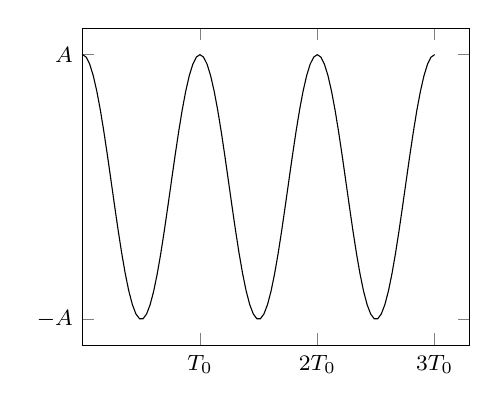
\begin{tikzpicture}
\begin{axis}[small,xmin=0,xtick={360,720,1080},xticklabels={$T_0$, $2T_0$,$3T_0$},ytick={-1,1},yticklabels={$-A$,$A$}]
\addplot[domain=0:1080,samples=100]{cos(x)};
\end{axis}
\end{tikzpicture}
\caption*{(الف) سائن نما موج۔}
\end{subfigure}%
\begin{subfigure}{0.5\textwidth}
\centering
\begin{tikzpicture}
\begin{axis}[small,xmin=0,xtick={1,3,6},xticklabels={$T_a$, $T_0$,$2T_0$},ytick={1},yticklabels={$A$}]
\addplot[] plot coordinates {(0,0) (0,1) (1,1) (1,0) (3,0) (3,1) (4,1) (4,0)(6,0) (6,1) (7,1) (7,0)};
\end{axis}%
\end{tikzpicture}
\caption*{(ب) مستطیل موج۔}
\end{subfigure}
\begin{subfigure}{0.5\textwidth}
\centering
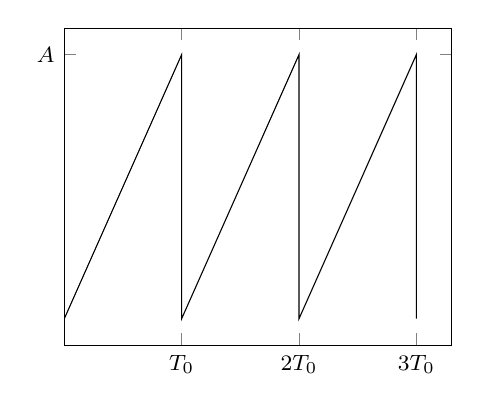
\begin{tikzpicture}
\begin{axis}[small,xmin=0,xtick={3,6,9},xticklabels={$T_0$, $2T_0$,$3T_0$},ytick={1},yticklabels={$A$}]
\addplot[] plot coordinates {(0,0) (3,1) (3,0) (6,1) (6,0) (9,1) (9,0)};
\end{axis}%
\end{tikzpicture}
\caption*{(پ) دندان موج۔}
\end{subfigure}%
\begin{subfigure}{0.5\textwidth}
\centering
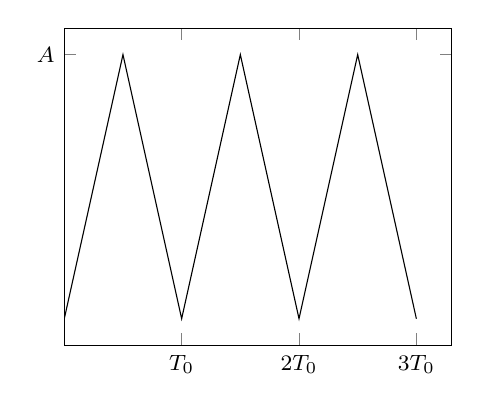
\begin{tikzpicture}
\begin{axis}[small,xmin=0,xtick={2,4,6},xticklabels={$T_0$, $2T_0$,$3T_0$},ytick={1},yticklabels={$A$}]
\addplot[] plot coordinates {(0,0) (1,1) (2,0) (3,1) (4,0) (5,1) (6,0)};
\end{axis}%
\end{tikzpicture}
\caption*{(ت) تکونی موج۔}
\end{subfigure}%
\caption{چند دوری امواج۔}
\label{شکل_فوریئر_چند_دوری_امواج}
\end{figure}

کسی بھی دوری تفاعل کو بطور درج ذیل (تکونیاتی) \اصطلاح{فوریئر تسلسل}\فرہنگ{فوریئر تسلسل!تکونیاتی}\فرہنگ{تسلسل!فوریئر}\حاشیہب{trignometric Fourier series}\فرہنگ{Fourier series!trignometric} لکھا\حاشیہد{جین بپٹسٹ یوسف فوریئر نے حرارتی توانائی کے بہاو پر غور کے دوران اس تسلسل کو دریافت کیا۔} جا سکتا ہے
\begin{gather}
\begin{aligned}\label{مساوات_فوریئر_تسلسل_سائن_نما_الف}
f(t)&=a_0+\sum_{n=1}^{\infty} [a_n \cos (n \omega_0 t) +b_n \sin (n \omega_0 t)]\\
&=a_0+a_1\cos \omega_0 t+a_2 \cos (2\omega_0 t)+a_3\cos (3\omega_0 t)+\cdots\\
&\phantom{=a_0\,\,}+b_1\sin \omega_0t+b_2\sin (2\omega_0t)+b_3 \sin (3\omega_0t)+\cdots
\end{aligned}
\end{gather}
جہاں \عددی{a_0}، \عددی{a_1}،\عددی{a_2}، \عددی{b_1} وغیرہ تسلسل کے \اصطلاح{عددی سر}\فرہنگ{عددی سر}\حاشیہب{coefficients}\فرہنگ{coefficients} کہلاتے ہیں۔فوریئر تسلسل کی اوسط قیمت \عددی{a_0} کے برابر ہے۔ایک دوری عرصہ \عددی{T_0} میں \عددی{\cos \omega_0 t} یا \عددی{\sin \omega_0 t} کی ایک لہر، \عددی{\cos (2\omega_0 t)} یا \عددی{\sin (2\omega_0 t)} کی دو لہریں اور \عددی{\cos (m\omega_0 t)} یا \عددی{\sin (m\omega_0 t)} کی \عددی{m} لہریں پوری آتی ہیں۔اس حقیقت کو شکل \حوالہ{شکل_فوریئر_ارکان_تعداد_فی_دوری_عرصہ} میں دکھایا گیا ہے جہاں وضاحت کی خاطر امواج کے حیطے مختلف رکھے گئے ہیں۔فوریئر تسلسل میں \عددی{a_1\cos \omega_0 t +b_1\sin \omega_0 t} \اصطلاح{بنیادی رکن}\فرہنگ{بنیادی رکن}\فرہنگ{ہارمونی!بنیادی رکن}\حاشیہب{fundamental component}\فرہنگ{fundamental component} یا \اصطلاح{پہلا ہارمونی رکن} کہلاتا ہے،   \عددی{a_2\cos (2\omega_0 t) +b_2\sin (2\omega_0 t)} \اصطلاح{دوسرا ہارمونی رکن}\فرہنگ{دوسرا ہارمونی رکن}\فرہنگ{ہارمونی!دوسرا رکن}\حاشیہب{second harmonic}\فرہنگ{harmonic!second} کہلاتا ہے،  \عددی{a_3\cos (3\omega_0 t) +b_3\sin (3\omega_0 t)} تیسرا ہارمونی رکن اور اسی طرح \عددی{a_m\cos (m\omega_0 t) +b_m\sin (m\omega_0 t)} ایم ہارمونی رکن کہلاتا ہے۔
\begin{figure}
\centering
\begin{tikzpicture}
\begin{axis}[kStyleCircuitsA,xlabel={$t\,(\si{\second})$},xtick={90,180,270,360},xticklabels={$\frac{1}{4}T_0$,$\frac{1}{2}T_0$,$\frac{3}{2}T_0$,$T_0$},ytick={1,-1},yticklabels={$+A_0$,$-A_0$}]
\addplot[mark=none,color=black,domain=0:360,samples=100]{sin(x)}node[pos=0.4,pin=45:{$A_0\sin \omega_0 t$}]{};
\addplot[mark=none,color=black,domain=0:360,samples=100]{0.5*sin(2*x)}node[pos=0.7,pin=45:{$\frac{A_0}{2}\sin 2\omega_0 t$}]{};
\end{axis}
\end{tikzpicture}
\caption{ایک دوری عرصہ میں فوریئر تسلسل کے ارکان کی تعداد۔}
\label{شکل_فوریئر_ارکان_تعداد_فی_دوری_عرصہ}
\end{figure}
%======================
ہم یہاں اصل رک کر چند حقائق اور تکملات پر غور کرتے ہیں جو فوریئر تسلسل میں کلیدی کردار ادا کرتے ہیں۔

آپ دو سمتیوں کے \اصطلاح{نقطہ ضرب}\فرہنگ{نقطہ ضرب}\فرہنگ{ضرب!نقطہ}\حاشیہب{dot product}\فرہنگ{dot product} سے خوب واقف ہیں۔سمتیہ \سمتیہ{A} اور \سمتیہ{B} کا نقطہ ضرب یا \اصطلاح{غیر سمتی ضرب}\فرہنگ{غیر سمتی ضرب}\فرہنگ{ضرب!غیر سمتی}\حاشیہب{scalar product}\فرہنگ{scalar product} درج ذیل ہے جہاں دونوں سمتیوں کے مابین زاویہ \عددی{\theta} ہے۔
\begin{align}
\kvec{A} \cdot \kvec{B}=A B \cos \theta
\end{align} 
آپس میں \اصطلاح{عمودی}\فرہنگ{عمودی}\حاشیہب{orthogonal}\فرہنگ{orthogonal} سمتیوں کے مابین \عددی{\theta=90^{\circ}} ہونے کی بدولت \عددی{\kvec{A} \cdot \kvec{B}=0} ہوتا ہے جبکہ کسی بھی سمتیہ کے خود نقطہ ضرب کا جذر اس کے حیطے  کے برابر ہوتا ہے۔
\begin{gather}
\begin{aligned}
 \abs{\kvec{A}}=\sqrt{\kvec{A} \cdot \kvec{A}}
\end{aligned}
\end{gather}
اسی سوچ کے ساتھ تفاعل کا نقطہ ضرب بیان کیا جاتا ہے۔

اگر تفاعل \عددی{f(t) \ne 0} اور \عددی{g(t)\ne 0} کے حاصل ضرب کا تکمل \عددی{a \le t \le b} فاصلے پر صفر کے برابر ہو
\begin{align}
\int_a^b f(t)g(t) \dif t=0
\end{align}
تو \عددی{a\le t\le b} فاصلے پر ان تفاعل کو آپس میں \اصطلاح{عمودی} تصور کیا جاتا ہے۔یاد رہے کہ دونوں تفاعل از خود \اصطلاح{غیر سمتی}\فرہنگ{غیر سمتی}\حاشیہب{scalar}\فرہنگ{scalar} اور غیر صفر ہیں۔

کسی بھی مقدار کا مربع مثبت ہوتا ہے لہٰذا تفاعل کا مربع \عددی{f^2(t)} ہر نقطے پر مثبت ہو گا۔ فاصلہ \عددی{a \le t \le b}  پر تفاعل کے \اصطلاح{معیار}\فرہنگ{معیار}\حاشیہب{norm}\فرہنگ{norm} \عددی{\parallel f(t) \parallel} سے مراد 
\begin{align}
\parallel f(t) \parallel =\sqrt{\int_a^b f^2(t) \dif t}
\end{align}
ہے۔
%===================
\ابتدا{مثال}
ثابت کریں کہ \عددی{0 \le t \le T_0}  فاصلے پر \عددی{\cos (m\omega_0 t)} اور \عددی{\cos (n\omega_0 t)} آپس میں عمودی ہیں جہاں \عددی{m=1,2,3,\cdots} اور \عددی{n=1,2,3,\cdots} ممکن ہیں لیکن \عددی{m\ne n} ہے۔

حل:دیے گئے فاصلے پر دونوں تفاعل کے حاصل ضرب کا تکمل لیتے ہیں۔
\begin{align*}
\int_0^{T_0} \cos (m\omega_0 t) \cos (n\omega_0 t) \dif t&=\int_0^{T_0} \frac{\cos\left[(m+n)\frac{2\pi}{T_0} t\right]+\cos\left[(m-n)\frac{2\pi}{T_0} t\right]}{2}\dif t\\
&=\left.\frac{\sin\left[(m+n)\frac{2\pi}{T_0} t\right]}{2(m+n)\frac{2\pi}{T_0} }+\frac{\sin\left[(m-n)\frac{2\pi}{T_0} t\right]}{2(m-n)\frac{2\pi}{T_0} }\right|_0^{T_0}\\
&=\frac{\sin[(m+n)2\pi]}{2(m+n)\frac{2\pi}{T_0} }+\frac{\sin[(m-n)2\pi]}{2(m-n)\frac{2\pi}{T_0} }\\
&\quad \quad \quad \quad -\frac{\sin[(m+n)0]}{2(m+n)\frac{2\pi}{T_0} }-\frac{\sin[(m-n)0]}{2(m-n)\frac{2\pi}{T_0} }
\end{align*}
چونکہ \عددی{m} اور \عددی{n} عدد صحیح ہیں لہٰذا \عددی{m+n} اور \عددی{m-n} بھی عدد صحیح ہوں گے لہٰذا \عددی{\sin[(m+n)2\pi]=0} اور \عددی{\sin[(m-n)2\pi]=0}  ہوں گے۔اس طرح درج ذیل حاصل ہوتا ہے جو عمودی تفاعل کو ظاہر کرتی ہے۔
\begin{align}\label{مساوات_فوریئر_مختلف_تکمل_الف}
\int_0^{T_0} \cos (m\omega_0 t) \cos (n\omega_0 t) \dif t=0\quad (m\ne n)
\end{align}
\انتہا{مثال}
%===================

\ابتدا{مثال}
ثابت کریں کہ \عددی{0 \le t \le T_0} فاصلے پر \عددی{\sin (m\omega_0 t)} اور \عددی{\sin (n\omega_0 t)} آپس میں عمودی ہیں جہاں \عددی{m=1,2,3,\cdots} اور \عددی{n=1,2,3,\cdots} ممکن ہیں لیکن \عددی{m\ne n} ہے۔

حل:دیے گئے فاصلے پر دونوں تفاعل کے حاصل ضرب کا تکمل لیتے ہیں۔
\begin{align*}
\int_0^{T_0} \sin (m\omega_0 t) \sin (n\omega_0 t) \dif t&=\int_0^{T_0} \frac{\cos\left[(m-n)\frac{2\pi}{T_0} t\right]-\cos\left[(m+n)\frac{2\pi}{T_0} t\right]}{2}\dif t\\
&=\left.\frac{\sin\left[(m-n)\frac{2\pi}{T_0} t\right]}{2(m-n)\frac{2\pi}{T_0} }-\frac{\sin\left[(m+n)\frac{2\pi}{T_0} t\right]}{2(m+n)\frac{2\pi}{T_0} }\right|_0^{T_0}\\
&=\frac{\sin[(m-n)2\pi]}{2(m-n)\frac{2\pi}{T_0} }-\frac{\sin[(m+n)2\pi]}{2(m+n)\frac{2\pi}{T_0} }\\
&\quad \quad \quad \quad -\frac{\sin[(m-n)0]}{2(m-n)\frac{2\pi}{T_0} }+\frac{\sin[(m+n)0]}{2(m+n)\frac{2\pi}{T_0} }
\end{align*}
چونکہ \عددی{m} اور \عددی{n} عدد صحیح ہیں لہٰذا \عددی{m+n} اور \عددی{m-n} بھی عدد صحیح ہوں گے لہٰذا \عددی{\sin[(m+n)2\pi]=0} اور \عددی{\sin[(m-n)2\pi]=0}  ہوں گے۔اس طرح درج ذیل حاصل ہوتا ہے جو عمودی تفاعل کو ظاہر کرتی ہے۔
\begin{align}\label{مساوات_فوریئر_مختلف_تکمل_ب}
\int_0^{T_0} \sin (m\omega_0 t) \sin (n\omega_0 t) \dif t=0\quad (m\ne n)
\end{align}
\انتہا{مثال}
%===================

\ابتدا{مثال}
ثابت کریں کہ \عددی{0 \le t \le T_0} فاصلے پر \عددی{\cos (m\omega_0 t)} اور \عددی{\sin (n\omega_0 t)} آپس میں عمودی ہیں جہاں \عددی{m=1,2,3,\cdots} اور \عددی{n=1,2,3,\cdots} ممکن ہیں۔

حل:دیے گئے فاصلے پر دونوں تفاعل کے حاصل ضرب کا تکمل لیتے ہیں۔
\begin{align*}
\int_0^{T_0} \cos (m\omega_0 t) \sin (n\omega_0 t) \dif t&=\frac{1}{2}\int_0^{T_0} \sin\left[(m+n)\frac{2\pi}{T_0} t\right]-\sin\left[(m-n)\frac{2\pi}{T_0} t\right]\dif t\\
&=\left.-\frac{\cos\left[(m+n)\frac{2\pi}{T_0} t\right]}{2(m+n)\frac{2\pi}{T_0}}+\frac{\cos\left[(m-n)\frac{2\pi}{T_0} t\right]}{2(m-n)\frac{2\pi}{T_0}}\right|_0^{T_0}\\
&=-\frac{\cos[(m+n)2\pi]}{2(m+n)\frac{2\pi}{T_0}}+\frac{\cos[(m-n)2\pi]}{2(m-n)\frac{2\pi}{T_0}}\\
&\quad \quad \quad \quad +\frac{\cos[(m+n)0]}{2(m+n)\frac{2\pi}{T_0}}-\frac{\cos[(m-n)0]}{2(m-n)\frac{2\pi}{T_0}}
\end{align*}
چونکہ \عددی{m} اور \عددی{n} عدد صحیح ہیں لہٰذا \عددی{m+n} اور \عددی{m-n} بھی عدد صحیح ہوں گے لہٰذا \عددی{\cos(m+n)2\pi=1} اور \عددی{\cos(m-n)2\pi=1}  ہوں گے۔اس طرح درج ذیل حاصل ہوتا ہے جو عمودی تفاعل کو ظاہر کرتی ہے۔
\begin{align}\label{مساوات_فوریئر_مختلف_تکمل_پ}
\int_0^{T_0} \cos (m\omega_0 t) \sin (n\omega_0 t) \dif t=0\quad (m\ne n)
\end{align}
\انتہا{مثال}
%===================
\ابتدا{مثال}
تفاعل \عددی{f(t)=\cos (m\omega_0 t)} کا معیار \عددی{0 \le t \le T_0} فاصلے پر حاصل کریں جہاں  \عددی{{m=1,2,3,\cdots}} ممکن ہے۔ 

حل:دیے گئے فاصلے پر معیار کو تکمل سے حاصل کرتے ہیں۔
\begin{align*}
\parallel f(t) \parallel^2&=\int_0^{T_0} \cos^2 \left(m\frac{2\pi}{T_0} t\right) \dif t\\
&=\frac{1}{2}\int_0^{T_0}\left[ 1+\cos \left(2m\frac{2\pi}{T_0} t\right)\right] \dif t\\
&=\left. \frac{t}{2}+\frac{\sin \left(2m\frac{2\pi}{T_0} t\right)}{4m\frac{2\pi}{T_0}}\right|_0^{T_0}\\
&=\frac{T_0}{2}+\frac{\sin 4m\pi}{4m\frac{2\pi}{T_0}}-\frac{0}{2}-\frac{\sin 0}{4m\frac{2\pi}{T_0}}\\
&=\frac{T_0}{2}
\end{align*}
دونوں اطراف کا جذر لیتے ہوئے  \عددی{0 \le t \le T_0} فاصلے پر معیار ملتا ہے۔
\begin{align}\label{مساوات_فوریئر_مختلف_تکمل_ت}
\parallel \cos (m\omega_0 t) \parallel =\sqrt{\int_0^{T_0} \cos^2  (m\omega_0 t) \dif t}=\sqrt{\frac{T_0}{2}}
\end{align}
\انتہا{مثال}
%==================

\ابتدا{مشق}
تفاعل \عددی{f(t)=\sin m\omega_0 t} کا معیار \عددی{0 \le t \le T_0} فاصلے پر درج ذیل ہے جہاں \عددی{m=1,2,3,\cdots} ممکن ہے۔ اس معیار کو حاصل کریں۔
\begin{align}\label{مساوات_فوریئر_مختلف_تکمل_ٹ}
\parallel \sin (m\omega_0 t) \parallel =\sqrt{\int_0^{T_0} \sin^2 (m\omega_0 t) \dif t}=\sqrt{\frac{T_0}{2}}
\end{align}
\انتہا{مشق}
%==================
\ابتدا{مشق}
درج ذیل دو مساوات کو ثابت کریں جہاں \عددی{m=1,2,3,\cdots} ممکن ہے۔
\begin{align}
\int_0^{T_0} \cos (m\omega_0 t) \dif t&=0 \label{مساوات_فوریئر_مختلف_تکمل_ث}\\
\int_0^{T_0} \sin (m\omega_0 t) \dif t&=0\label{مساوات_فوریئر_مختلف_تکمل_ج}
\end{align}
\انتہا{مشق}
%====================
مساوات \حوالہ{مساوات_فوریئر_مختلف_تکمل_الف}، مساوات \حوالہ{مساوات_فوریئر_مختلف_تکمل_ب} اور مساوات \حوالہ{مساوات_فوریئر_مختلف_تکمل_پ} مل کر ثابت کرتے ہیں کہ فوریئر تسلسل میں استعمال ہونے والا ہر تفاعل بقایا تمام تفاعل کے ساتھ \عددی{0 \le t \le T_0} فاصلے پر عمودی ہے۔یوں \عددی{\cos (3\omega_0 t)} کو مثال بناتے ہوئے ہم دیکھتے ہیں کہ یہ \عددی{\cos \omega_0 t}، \عددی{\cos(2\omega_0 t)}،\عددی{\cos(4\omega_0 t)}، \عددی{\sin\omega_0 t}، \عددی{\sin(2\omega_0 t)}، \عددی{\sin(3\omega_0 t)} وغیرہ کے ساتھ عمودی ہے۔

%====================
درج بالا تکملات حاصل کرنے کے بعد اصل مضمون یعنی فوریئر تسلسل پر دوبارہ آتے ہیں۔مساوات \حوالہ{مساوات_فوریئر_مختلف_تکمل_الف} تا مساوات \حوالہ{مساوات_فوریئر_مختلف_تکمل_ج} کو استعمال کرتے ہوئے مساوات  \حوالہ{مساوات_فوریئر_تسلسل_سائن_نما_الف} کے عددی سر \عددی{a_0, a_1,a_2,b_1,\cdots} حاصل کئے جا سکتے ہیں۔آئیں ایسا ہی کریں۔

عددی سر \عددی{a_0} کی قیمت دریافت کرنے کی خاطر ہم  مساوات  \حوالہ{مساوات_فوریئر_تسلسل_سائن_نما_الف} کا تکمل \عددی{0 \le t \le T_0} فاصلے پر لیتے ہیں
\begin{align*}
\int_0^{T_0}f(t) \dif t&=\int_0^{T_0} a_0 \dif t+\sum_{n=1}^{\infty}  \int_0^{T_0}(a_n\cos n \omega_0 t +b_n \sin n \omega_0 t) \dif t\\
&=a_0 T_0
\end{align*}
جہاں مساوات \حوالہ{مساوات_فوریئر_مختلف_تکمل_ث} اور مساوات \حوالہ{مساوات_فوریئر_مختلف_تکمل_ج} کو استعمال کرتے ہوئے مجموعے میں دیے تمام تکمل کو صفر کے برابر پر کیا گیا ہے۔ یوں درج ذیل حاصل ہوتا ہے۔
\begin{align}\label{مساوات_فوریئر_عددی_سر_الف}
a_0=\frac{1}{T_0}\int_0^{T_0}f(t) \dif t
\end{align}
مساوات \حوالہ{مساوات_فوریئر_عددی_سر_الف} کہتا ہے کہ \عددی{a_0} تفاعل \عددی{f(t)} کی اوسط قیمت ہے۔


عددی سر \عددی{a_m} حاصل کرنے کی خاطر مساوات \حوالہ{مساوات_فوریئر_تسلسل_سائن_نما_الف} کے دونوں اطراف کو \عددی{\cos (m\omega_0t)} سے ضرب دیتے ہوئے ایک دوری عرصے پر تکمل کرتے ہیں۔ہم تکمل کو \عددی{0 \le t \le T_0} پر حاصل کرتے ہیں۔
\begin{multline}\label{مساوات_فوریئر_عددی_سر_کا_حصول_الف}
\int_0^{T_0}f(t) \cos( m \omega_0 t) \dif t=\\
\int_0^{T_0} a_0 \cos (m\omega_0 t) \dif t+\sum_{n=1}^{\infty}  \int_0^{T_0} a_n\cos (n \omega_0 t)  \cos (m \omega_0 t) \dif t \\
+\sum_{n=1}^{\infty} \int_0^{T_0} b_n \sin (n \omega_0 t) \cos (m\omega_0 t) \dif t
\end{multline}
دائیں ہاتھ پہلا تکمل مساوات \حوالہ{مساوات_فوریئر_مختلف_تکمل_ث} کی بنا صفر کے برابر ہے جبکہ مساوات \حوالہ{مساوات_فوریئر_مختلف_تکمل_پ} کے تحت تیسرا تکمل صفر کے برابر ہے۔آئیں دوسرے تکمل پر غور کریں۔
\begin{multline*}
\sum_{n=1}^{\infty}  \int_0^{T_0} a_n\cos n \omega_0 t  \cos m \omega_0 t \dif t =\\
\int_0^{T_0} \cos (m\omega_0 t)\left[a_1 \cos \omega_0 t+a_2\cos (2\omega_0 t)+\cdots \right.\\
\left.+a_{m-1}\cos[(m-1)\omega_0 t]+a_m\cos(m\omega_0 t)+\cdots \right] \dif t
\end{multline*}
اب اگر \عددی{n \ne m} ہو تب مساوات \حوالہ{مساوات_فوریئر_مختلف_تکمل_الف} کے تحت تکمل صفر کے برابر ہو گا۔البتہ \عددی{n=m} کی صورت میں مساوات \حوالہ{مساوات_فوریئر_مختلف_تکمل_ت} کو استعمال کرتے ہوئے
\begin{align*}
\int_0^{T_0}a_m \cos^2 (m\omega_0 t) \dif t=a_m\frac{T_0}{2}
\end{align*} 
حاصل ہوتا ہے۔ان قیمتوں کو مساوات \حوالہ{مساوات_فوریئر_عددی_سر_کا_حصول_الف} میں پر کرتے ہوئے درج ذیل حاصل ہوتا ہے۔
\begin{align}\label{مساوات_فوریئر_عددی_سر_ب}
a_m=\frac{2}{T_0}\int_0^{T_0}f(t) \cos (m \omega_0 t) \dif t
\end{align}

عددی سر \عددی{b_m} حاصل کرنے کی خاطر مساوات \حوالہ{مساوات_فوریئر_تسلسل_سائن_نما_الف} کے دونوں اطراف کو \عددی{\sin (m\omega_0 t)} سے ضرب دیتے ہوئے ایک دوری عرصے پر تکمل کرتے ہیں۔ہم تکمل کو \عددی{0 \le t \le T_0} پر حاصل کرتے ہیں۔
\begin{multline}\label{مساوات_فوریئر_عددی_سر_کا_حصول_ب}
\int_0^{T_0}f(t) \sin (m \omega_0 t) \dif t=\\
\int_0^{T_0} a_0 \sin (m\omega_0 t) \dif t+\sum_{n=1}^{\infty}  \int_0^{T_0} a_n\cos (n \omega_0 t)  \sin (m \omega_0 t) \dif t \\
+\sum_{n=1}^{\infty} \int_0^{T_0} b_n \sin (n \omega_0 t) \sin (m\omega_0 t) \dif t
\end{multline}
دائیں ہاتھ پہلا تکمل مساوات \حوالہ{مساوات_فوریئر_مختلف_تکمل_ج} کی بنا صفر کے برابر ہے جبکہ مساوات \حوالہ{مساوات_فوریئر_مختلف_تکمل_پ} کے تحت دوسرا تکمل صفر کے برابر ہے۔آئیں تیسرے تکمل پر غور کریں۔
\begin{multline*}
\sum_{n=1}^{\infty} \int_0^{T_0} b_n \sin (n \omega_0 t) \sin (m\omega_0 t) \dif t=\\
\int_0^{T_0} \sin (m\omega_0 t)\left[b_1 \sin \omega_0 t+b_2\sin (2\omega_0 t)+\cdots \right.\\
\left.+b_{m-1}\sin[(m-1)\omega_0 t]+b_m\sin(m\omega_0 t)+\cdots \right] \dif t
\end{multline*}
اب اگر \عددی{n \ne m} ہو تب مساوات \حوالہ{مساوات_فوریئر_مختلف_تکمل_ب} کے تحت تکمل صفر کے برابر ہو گا۔البتہ \عددی{n=m} کی صورت میں مساوات \حوالہ{مساوات_فوریئر_مختلف_تکمل_ٹ} کو استعمال کرتے ہوئے
\begin{align*}
\int_0^{T_0}b_m \sin^2 (m\omega_0 t) \dif t=b_m\frac{T_0}{2}
\end{align*} 
حاصل ہوتا ہے۔ان قیمتوں کو مساوات \حوالہ{مساوات_فوریئر_عددی_سر_کا_حصول_الف} میں پر کرتے ہوئے درج ذیل حاصل ہوتا ہے۔
\begin{align}\label{مساوات_فوریئر_عددی_سر_پ}
b_m=\frac{2}{T_0}\int_0^{T_0}f(t) \sin (m \omega_0 t) \dif t
\end{align}
مساوات \حوالہ{مساوات_فوریئر_عددی_سر_الف}، مساوات \حوالہ{مساوات_فوریئر_عددی_سر_ب} اور مساوات \حوالہ{مساوات_فوریئر_عددی_سر_پ} فوریئر تکمل کے عددی سر دیتے ہیں۔انہیں یہاں اکٹھے پیش کرتے ہیں۔
\begin{gather}
\begin{aligned}\label{مساوات_فوریئر_عددی_سر_ت}
a_0&=\frac{1}{T_0}\int_0^{T_0}f(t) \dif t\\
a_m&=\frac{2}{T_0}\int_0^{T_0}f(t) \cos (m \omega_0 t) \dif t\\
b_m&=\frac{2}{T_0}\int_0^{T_0}f(t) \sin (m \omega_0 t) \dif t
\end{aligned}
\end{gather}
%============

\ابتدا{مثال}\شناخت{مثال_فوریئر_دندان_موج_الف}
شکل \حوالہ{شکل_فوریئر_دندان_موج_الف}-الف میں دکھائے گئے \اصطلاح{دندان موج}\فرہنگ{دندان موج}\فرہنگ{موج!دندان}\فرہنگ{saw tooth} کا فوریئر تسلسل حاصل کریں۔دو، پانچ اور پچاس فوریئر ارکان استعمال کرتے ہوئے  موج کا خط کھینچیں۔آپ دیکھ سکتے ہیں کہ موج کا دوری عرصہ \عددی{T_0=\SI{3}{\second}} ہے۔
\begin{figure}
\centering
\begin{subfigure}{0.5\textwidth}
\centering
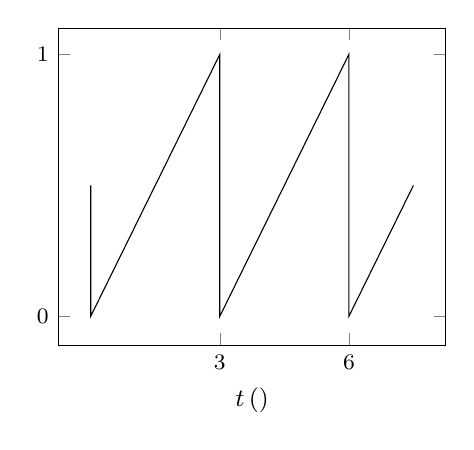
\begin{tikzpicture}
\begin{axis}[small,xlabel={$t\,(\second)$},ylabel style={rotate=-90},xtick={3,6},xticklabels={$3$,$6$},ytick={0,1},yticklabels={$0$,$1$},ymax=1.1]
\addplot[] plot coordinates {(0,0.5)(0,0)  (3,1)  (3,0) (6,1) (6,0) (7.5,0.5)};
\end{axis}
\end{tikzpicture}
\caption*{(الف) دندان موج۔}
\end{subfigure}%
\begin{subfigure}{0.5\textwidth}
\centering
\includegraphics{figFourierSawTooth2}
\caption*{(ب) دو ہارمونی ارکان شامل کئے گئے ہیں۔}
\end{subfigure}
\begin{subfigure}{0.5\textwidth}
\centering
\includegraphics{figFourierSawTooth5}
\caption*{(پ) پانچ ہارمونی ارکان شامل کئے گئے ہیں۔}
\end{subfigure}%
\begin{subfigure}{0.5\textwidth}
\centering
\includegraphics{figFourierSawTooth50}
\caption*{(ت) پچاس ہارمونی ارکان شامل کئے گئے ہیں۔}
\end{subfigure}%
\caption{مثال \حوالہ{مثال_فوریئر_دندان_موج_الف} کی دندان موج۔}
\label{شکل_فوریئر_دندان_موج_الف}
\end{figure}

حل:شکل میں دکھائی گئی موج \عددی{(0,0)} سے \عددی{(3,1)} تک بالکل سیدھی لکیر کی مانند ہے جس کی ڈھلوان 
\begin{align*}
\text{ڈھلوان}=\frac{y_2-y_1}{x_2-x_1}=\frac{1-0}{3-0}=\frac{1}{3}
\end{align*}
ہے لہٰذا اس سیدھے حصے کی مساوات درج ذیل لکھی جا سکتی ہے جہاں لکیر پر کسی بھی نقطے کے کارتیسی محدد مساوات میں پر کرنے سے \عددی{c} کی قیمت حاصل کی جا سکتی ہے۔
\begin{align*}
y=\frac{x}{3}+c
\end{align*}
ہم درج بالا میں \عددی{(0,0)} پر کرتے ہوئے
\begin{align*}
0=\frac{0}{3}+c
\end{align*}
 \عددی{c=0} حاصل کرتے ہیں لہٰذا سیدھی حصے کی مساوات \عددی{y=\tfrac{x}{3}} یعنی
\begin{align}
f(t)=\frac{t}{3}
\end{align}
ہے جہاں کارتیسی نظام کے \عددی{x} محور پر \عددی{t} اور \عددی{y} محور پر \عددی{f(t)} پر کئے گئے ہیں۔

مساوات \حوالہ{مساوات_فوریئر_عددی_سر_ت} سے فوریئر تسلسل کے عددی سر حاصل کرتے ہیں۔
\begin{align*}
a_0&=\frac{1}{T_0}\int_0^{T_0} f(t) \dif t\\
&=\frac{1}{3}\int_0^3 \frac{t}{3} \dif t\\
&=\left. \frac{1}{3} \frac{t^2}{6} \right|_0^3\\
&=\frac{1}{2}
\end{align*}
چونکہ \عددی{a_0} تفاعل کی اوسط قیمت کے برابر ہے لہٰذا یہی جواب تکون کے رقبے \عددی{\tfrac{1}{2}\times 3\times 1=\tfrac{3}{2}} اور قاعدہ \عددی{3} سے حاصل کی جا سکتی ہے یعنی
\begin{align*}
\text{اوسط}&=\frac{\text{رقبہ}}{\text{قاعدہ}}=\frac{\frac{3}{2}}{3}=\frac{1}{2}
\end{align*}
عددی سر \عددی{a_m} حاصل کرتے ہیں۔
\begin{align*}
a_m&=\frac{2}{T_0}\int_0^{T_0} f(t)\cos (m\omega_0 t) \dif t\\
&=\frac{2}{3}\int_0^3 \frac{t}{3} \cos (m \frac{2\pi}{3} t) \dif t\\
&=\left. \frac{2}{9}t \frac{\sin(\frac{2\pi}{3}mt)}{\frac{2\pi}{3}m}+\frac{2}{9}\frac{\cos(\frac{2\pi}{3}mt)}{\left(\frac{2\pi}{3}m\right)^2}\right|_0^3\\
&=0
\end{align*}
اس کا مطلب ہے کہ دندان موج کی فوریئر تسلسل میں کوئی کوسائن تفاعل نہیں پایا جاتا۔

عددی سر \عددی{b_m} حاصل کرتے ہیں۔
\begin{align*}
b_m&=\frac{2}{T_0}\int_0^{T_0} f(t)\sin(m\omega_0 t) \dif t\\
&=\frac{2}{3}\int_0^3 \frac{t}{3}\sin (m\frac{2\pi}{3} t) \dif t\\
&=\left.-\frac{2}{9}t\frac{\cos(\frac{2\pi}{3}mt)}{\frac{2\pi}{3}m}+\frac{2}{9}\frac{\sin(\frac{2\pi}{3}mt)}{\left(\frac{2\pi}{3}m\right)^2}\right|_0^3\\
&=-\frac{1}{m\pi}
\end{align*}
یوں \عددی{m=1,2,3,\cdots} پر کرتے ہوئے عددی سر حاصل ہوتے ہیں یعنی
\begin{align*}
b_1&=-\frac{1}{\pi}\\
b_2&=-\frac{1}{2\pi}\\
b_3&=-\frac{1}{3\pi}\\
&\vdots
\end{align*}
لہٰذا فوریئر تسلسل درج ذیل لکھی جائے گی۔
\begin{align}\label{مساوات_فوریئر_دندان_موج}
f(t)=\frac{1}{2}-\frac{1}{\pi}\left[\sin \omega_0 t+\frac{1}{2} \sin (2\omega_0 t) +\frac{1}{3} \sin (3\omega_0 t)+\cdots\right]
\end{align}
شکل \حوالہ{شکل_فوریئر_دندان_موج_الف}-ب میں  مساوات \حوالہ{مساوات_فوریئر_دندان_موج} کو \عددی{m=2} تک استعمال کرتے ہوئے خط کھینچا گیا ہے۔شکل-پ میں پانچ ہارمونی ارکان استعمال کئے گئے ہیں جبکہ شکل-ت میں پچاس ہارمونی ارکان استعمال کئے گئے ہیں۔آپ دیکھ سکتے ہیں کہ ارکان بڑھانے سے اصل موج کے قریب تر خط حاصل کیا جا سکتا ہے۔
\انتہا{مثال}
%========================
\ابتدا{مثال}\شناخت{مثال_فوریئر_مستطیل_موج}
آئیں شکل \حوالہ{شکل_فوریئر_مستطیل_موج_الف}-الف  میں دکھائے گئے  دوری مستطیل موج کا فوریئر تسلسل حاصل کریں جس میں دوری عرصے کو \عددی{T} لکھا گیا ہے۔
\begin{figure}
\centering
\begin{subfigure}{0.5\textwidth}
\centering
\begin{tikzpicture}
\begin{axis}[small,xlabel={$t$},ylabel style={rotate=-90},xtick={-2,-1,0,1,2,3},xticklabels={$-\frac{T}{2}$,$-\frac{T}{4}$,$0$,$\frac{T}{4}$,$\frac{T}{2}$,$\frac{3T}{4}$},ytick={-1,1},yticklabels={$-V_0$,$V_0$}]
\addplot[] plot coordinates {(-4,1) (-3,1) (-3,-1) (-1,-1) (-1,1) (1,1) (1,-1) (3,-1) (3,1)(4,1)};
\end{axis}
\end{tikzpicture}
\caption*{(الف) مستطیل موج۔}
\end{subfigure}%
\begin{subfigure}{0.5\textwidth}
\centering
\includegraphics{figFourierSquareWave5}
\caption*{(ب) ایک، تین اور پانچ ہارمونی ارکان کا مجموعہ یعنی \عددی{m=5} ہے۔}
\end{subfigure}
\begin{subfigure}{0.5\textwidth}
\centering
\includegraphics{figFourierSquareWave10}
\caption*{((پ) \عددی{m=9} تک ارکان کا مجموعہ۔}
\end{subfigure}%
\begin{subfigure}{0.5\textwidth}
\centering
\includegraphics{figFourierSquareWave50}
\caption*{(ت) \عددی{m=49} تک ارکان کا مجموعہ۔}
\end{subfigure}
\caption{مثال \حوالہ{مثال_فوریئر_مستطیل_موج} کی مستطیل موج۔}
\label{شکل_فوریئر_مستطیل_موج_الف}
\end{figure}

حل:افقی محور کے دونوں اطراف برابر موج پائی جاتی ہے لہٰذا اس کی اوسط قیمت صفر ہو گی اور یوں \عددی{a_0=0} ہو گا۔آئیں یہی جواب مساوات \حوالہ{مساوات_فوریئر_عددی_سر_ت} سے حاصل کریں۔اس مرتبہ ہم دوری عرصے کو \عددی{-\tfrac{T}{2} \le t \le \tfrac{T}{2}} لیتے ہیں۔شکل کو دیکھ معلوم ہوتا ہے کہ \عددی{-\tfrac{T}{4} \le t \le \tfrac{T}{4}} تفاعل کی قیمت \عددی{V_0} ہے جبکہ
 \عددی{-\frac{T}{2}\le t \le -\tfrac{T}{4}} اور \عددی{\tfrac{T}{4} \le t \le \tfrac{T}{2}} پر تفاعل کی قیمت \عددی{-V_0} ہے۔
\begin{align*}
a_0&=\frac{1}{T}\int_0^T f(t) \dif t\\
&=\frac{1}{T} \left(-V_0 \int_{-\frac{T}{2}}^{-\frac{T}{4}} \dif t+V_0\int_{-\frac{T}{4}}^{\frac{T}{4}}\dif t -V_0\int_{\frac{T}{4}}^{\frac{T}{2}} \dif t\right)\\
&=\frac{1}{T}\left[-V_0\left(-\frac{T}{4}+\frac{T}{2}\right)+V_0\left(\frac{T}{4}+\frac{T}{4}\right)-V_0\left(\frac{T}{2}-\frac{T}{4}\right)\right]\\
&=0
\end{align*}
کوسائن کے عددی سر \عددی{a_m} کو مساوات \حوالہ{مساوات_فوریئر_عددی_سر_ت} کی مدد سے حاصل کرتے ہیں۔مستقل \عددی{V_0} کو تکمل کے باہر لکھا گیا ہے۔
\begin{align*}
a_m&=\frac{2}{T}\int_0^T f(t)\cos(m\omega_0 t) \dif t\\
&=-\frac{2}{T}V_0\int_{-\frac{T}{2}}^{-\frac{T}{4}} \cos (\frac{2\pi m}{T} t) \dif t+\frac{2}{T}V_0\int_{-\frac{T}{4}}^{\frac{T}{4}} \cos (\frac{2\pi m}{T} t) \dif t-\frac{2}{T}V_0\int_{\frac{T}{4}}^{\frac{T}{2}} \cos (\frac{2\pi m}{T} t) \dif t\\
&=-\frac{2V_0}{T}\left.\frac{\sin (\frac{2\pi m}{T} t)}{\frac{2\pi m}{T}}\right|_{-\frac{T}{2}}^{-\frac{T}{4}}+\frac{2V_0}{T}\left.\frac{\sin (\frac{2\pi m}{T} t)}{\frac{2\pi m}{T}}\right|_{-\frac{T}{4}}^{\frac{T}{4}}-\frac{2V_0}{T}\left.\frac{\sin (\frac{2\pi m}{T} t)}{\frac{2\pi m}{T}}\right|_{\frac{T}{4}}^{\frac{T}{2}}\\
&=\frac{4V_0}{m\pi} \sin(\frac{m\pi}{2})
\end{align*}
اس سے درج ذیل عددی سر لکھے جا سکتے ہیں۔
\begin{align*}
a_1&=\frac{4V_0}{1\pi} \sin(\frac{1\pi}{2})=\frac{4V_0}{\pi}\\
a_2&=\frac{4V_0}{2\pi} \sin(\frac{2\pi}{2})=0\\
a_3&=\frac{4V_0}{3\pi} \sin(\frac{3\pi}{2})=-\frac{4V_0}{3\pi}\\
a_4&=\frac{4V_0}{4\pi} \sin(\frac{4\pi}{2})=0\\
a_5&=\frac{4V_0}{5\pi} \sin(\frac{5\pi}{2})=\frac{4V_0}{5\pi}\\
&\vdots
\end{align*}
سائن کے عددی سر \عددی{b_m} کو مساوات \حوالہ{مساوات_فوریئر_عددی_سر_ت} کی مدد سے حاصل کرتے ہیں۔مستقل \عددی{V_0} کو تکمل کے باہر لکھا گیا ہے۔
\begin{align*}
b_m&=\frac{2}{T}\int_0^T f(t)\sin(m\omega_0 t) \dif t\\
&=-\frac{2}{T}V_0\int_{-\frac{T}{2}}^{-\frac{T}{4}} \sin (\frac{2\pi m}{T} t) \dif t+\frac{2}{T}V_0\int_{-\frac{T}{4}}^{\frac{T}{4}} \sin (\frac{2\pi m}{T} t) \dif t-\frac{2}{T}V_0\int_{\frac{T}{4}}^{\frac{T}{2}} \sin (\frac{2\pi m}{T} t) \dif t\\
&=\frac{2V_0}{T}\left.\frac{\cos (\frac{2\pi m}{T} t)}{\frac{2\pi m}{T}}\right|_{-\frac{T}{2}}^{-\frac{T}{4}}-\frac{2V_0}{T}\left.\frac{\cos (\frac{2\pi m}{T} t)}{\frac{2\pi m}{T}}\right|_{-\frac{T}{4}}^{\frac{T}{4}}+\frac{2V_0}{T}\left.\frac{\cos (\frac{2\pi m}{T} t)}{\frac{2\pi m}{T}}\right|_{\frac{T}{4}}^{\frac{T}{2}}\\
&=0
\end{align*}
اس معلومات کو استعمال کرتے ہوئے مستطیل موج کی فوریئر مساوات لکھتے ہیں۔
\begin{align}\label{مساوات_فوریئر_مستطیل_موج}
f(t)=\frac{4V_0}{\pi}\left[\cos \omega_0 t-\frac{1}{3}\cos(3\omega_0 t)+\frac{1}{5}\cos(5\omega_0 t)-\frac{1}{7}\cos(7\omega_0 t)+\cdots\right]
\end{align}
مختلف تعداد میں فوریئر تسلسل کے ارکان شامل کرتے ہوئے تفاعل کو شکل \حوالہ{شکل_فوریئر_مستطیل_موج_الف}-ب تا شکل \حوالہ{شکل_فوریئر_مستطیل_موج_الف}-ت میں دکھایا گیا ہے۔
\انتہا{مثال}
%=======================

مثال \حوالہ{مثال_فوریئر_مستطیل_موج} میں مستطیل موج کی فوریئر تسلسل  حاصل کی گئی۔آئیں تسلسل کے ایک رکن سے شروع کرتے ہوئے دیکھیں کہ اس میں مزید ارکان شامل کرتے ہوئے مستطیل موج کیسے حاصل ہوتی ہے۔شکل \حوالہ{شکل_فوریئر_ابھرتا_مستطیل}-الف میں  مساوات \حوالہ{مساوات_فوریئر_مستطیل_موج} کا پہلا ہارمونی رکن \عددی{\tfrac{4V_0}{\pi}\cos\omega_0 t} اور تیسرا ہارمونی رکن \عددی{-\frac{4V_0}{3\pi}\cos(3\omega_0t)} ہلکی سیاہی میں دکھائے گئے ہیں۔دونوں سائن نما صورت رکھتے ہیں جس کا مستطیل سے دور دور تک کوئی واسطہ نہیں ہے۔اسی شکل میں دونوں کے مجموعے کو گہری سیاہی میں دکھایا گیا ہے۔آپ دیکھ سکتے ہیں کہ دو سائن نما امواج مل کر ایسی شکل بناتے ہیں جو مستطیل زیادہ اور سائن نما کم نظر آتا ہے۔مستطیل موج کی چوٹی \عددی{V_0} ہے جبکہ پہلے ہارمونی رکن کی چوٹی \عددی{\tfrac{4V_0}{\pi}=1.27V_0} ہے۔تیسرا ہارمونی رکن اس چوٹی کو نیچے کھینچتا ہے۔اسی طرح مستطیل موج \عددی{\mp \tfrac{T}{4}} پر یکدم قیمت تبدیل کرتی ہے جبکہ پہلا ہارمونی جزو نہایت صبروتحمل کے ساتھ منفی چوٹی سے مثبت چوٹی اور مثبت چوٹی سے منفی چوٹی پہنچتی ہے۔ یہاں بھی تیسرا ہارمونی رکن پہلے رکن کے اطراف کو کھینچ کر ان کی ڈھلوان بڑھاتی ہے۔

\begin{figure}
\centering
\begin{subfigure}{0.5\textwidth}
\centering
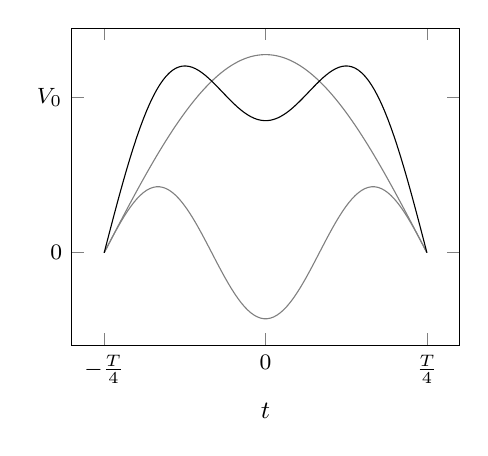
\begin{tikzpicture}
\begin{axis}[small,xlabel={$t$},ylabel style={rotate=-90},xtick={-2,-1,0,1,2},xticklabels={$-\frac{T}{2}$,$-\frac{T}{4}$,$0$,$\frac{T}{4}$,$\frac{T}{2}$},ytick={0,1},yticklabels={$0$,$V_0$}]
\addplot[gray,domain=-1:1,samples=100]{4/pi*cos(90*x)};
\addplot[gray,domain=-1:1,samples=100]{-4/(3*pi)*cos(3*90*x)};
\addplot[black,domain=-1:1,samples=100]{4/pi*cos(90*x)-4/(3*pi)*cos(3*90*x)};
\end{axis}
\end{tikzpicture}
\caption*{(الف) پہلا اور تیسرا ہارمونی رکن مل کر مستطیل صورت بنانے کی کوشش کرتے ہیں۔}
\end{subfigure}%
\begin{subfigure}{0.5\textwidth}
\centering
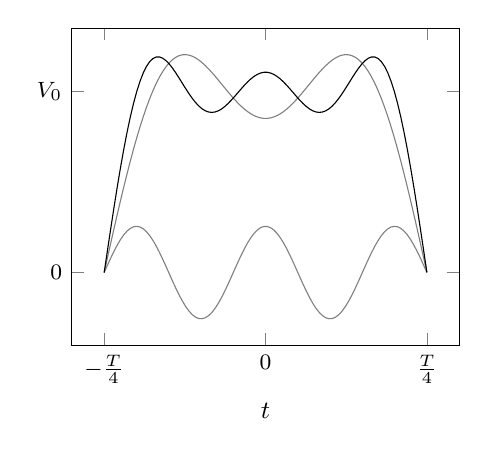
\begin{tikzpicture}
\begin{axis}[small,xlabel={$t$},ylabel style={rotate=-90},xtick={-2,-1,0,1,2},xticklabels={$-\frac{T}{2}$,$-\frac{T}{4}$,$0$,$\frac{T}{4}$,$\frac{T}{2}$},ytick={0,1},yticklabels={$0$,$V_0$}]
\addplot[gray,domain=-1:1,samples=100]{4/pi*cos(90*x)-4/(3*pi)*cos(3*90*x)};
\addplot[gray,domain=-1:1,samples=100]{4/(5*pi)*cos(5*90*x)};
\addplot[black,domain=-1:1,samples=100]{4/pi*cos(90*x)-4/(3*pi)*cos(3*90*x)+4/(5*pi)*cos(5*90*x)};
\end{axis}
\end{tikzpicture}
\caption*{(ب) پہلے،تیسرا اور پانچواں ہارمونی ارکان مل کر مستطیل شکل بناتے ہیں۔}
\end{subfigure}
\caption{بتدریج زیادہ ارکان شامل کرتے ہوئے مستطیل موج کی صورت ابھرتے ہوئے دیکھتے ہیں۔}
\label{شکل_فوریئر_ابھرتا_مستطیل}
\end{figure}

شکل \حوالہ{شکل_فوریئر_ابھرتا_مستطیل}-الف میں تیسرا رکن زیادہ جزبات میں آ کر پہلی رکن کی چوٹی ضرورت سے زیادہ نیچے کھینچ  دیتا ہے۔شکل-ب میں پہلے اور تیسرے ارکان سے حاصل موج کو ہلکی سیاہی میں دکھایا گیا ہے۔ساتھ ہی ساتھ پانچویں رکن کو بھی ہلکی سیاہی میں دکھایا گیا ہے۔ان کے مجموعے کو گہری سیاہی میں دکھایا گیا ہے۔آپ دیکھ سکتے ہیں پانچواں رکن ضرورت سے زیادہ نیچے کھینچی گئی چوٹی کو معمولی اٹھاتا ہے تا کہ یہ \عددی{V_0} کے قریب ہو جائے۔اسی طرح یہ رکن بھی موج کے اطراف کی ڈھلوان بڑھاتا ہے۔فوریئر تسلسل کے بقایا ارکان بھی اسی طرح مدد کرتے ہوئے اطراف کو زیادہ عمودی اور چوٹی کو بالکل چپٹی بنانے میں مدد دیتے ہیں حتٰی کہ ہمیں بالکل مستطیل موج نظر آتی ہے۔

شکل \حوالہ{شکل_فوریئر_مستطیل_موج_الف}-ب، پ اور ت میں آپ دیکھتے ہیں کہ فوریئر تسلسل سے حاصل موج \عددی{\mp \tfrac{T}{4}} پر درکار قیمت سے تجاوز کرتے ہوئے آگے نکل جاتی ہے۔تسلسل میں ارکان کی تعداد بڑھانے سے ان تجاوزات کا خاتمہ نہیں ہوتا۔
%======================
\ابتدا{مشق}
شکل \حوالہ{شکل_فوریئر_مستطیل_موج_الف}-الف میں عددی سر حاصل کرتے ہوئے تکملات کو \عددی{-\tfrac{T}{4}\le t\le \tfrac{3T}{4}} پر حاصل کرتے ہوئے فوریئر تسلسل حاصل کریں۔

جواب:عددی سر حاصل کرتے ہوئے دوری موج کے کسی بھی حصے پر مسلسل ایک دوری عرصے پر تکمل حاصل کیا جا سکتا ہے۔جوابات میں کوئی فرق نہیں پایا جاتا۔
\انتہا{مشق}
%=======================
\ابتدا{مشق}\شناخت{مشق_فوریئر_مشق_مستطیل}
شکل \حوالہ{شکل_فوریئر_مشق_مستطیل}-الف میں دکھائے گئے مستطیل موج کی فوریئر تسلسل حاصل کریں۔
\begin{figure}
\centering
\begin{subfigure}{0.5\textwidth}
\centering
\begin{tikzpicture}
\begin{axis}[small,xlabel={$t$},ylabel style={rotate=-90},xtick={0,1,2},xticklabels={$0$,$\frac{T}{2}$,$T$},ytick={-1,0,1},yticklabels={$-V_0$,$0$,$V_0$}]
\addplot[] plot coordinates{(-0.25,-1) (0,-1) (0,1) (1,1) (1,-1) (2,-1) (2,1) (3,1) (3,-1) (3.25,-1)};
\end{axis}
\end{tikzpicture}
\caption*{(الف) مستطیل موج۔}
\end{subfigure}%
\begin{subfigure}{0.5\textwidth}
\centering
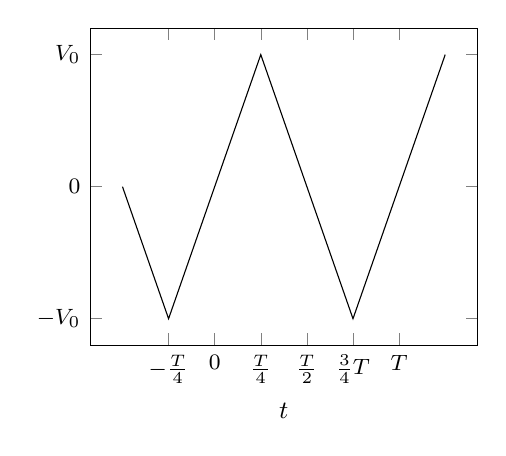
\begin{tikzpicture}
\begin{axis}[small,xlabel={$t$},ylabel style={rotate=-90},xtick={-1,0,1,2,3,4},xticklabels={$-\frac{T}{4}$,$0$,$\frac{T}{4}$,$\frac{T}{2}$,$\frac{3}{4}T$,$T$},ytick={-1,0,1},yticklabels={$-V_0$,$0$,$V_0$}]
\addplot[] plot coordinates{(-2,0)(-1,-1) (1,1) (3,-1) (5,1) };
\end{axis}
\end{tikzpicture}
\caption*{(ب) تکونی موج۔}
\end{subfigure}
\caption{مشق \حوالہ{مشق_فوریئر_مشق_مستطیل} اور مشق \حوالہ{مشق_فوریئر_مشق_تکونی} کے امواج۔}
\label{شکل_فوریئر_مشق_مستطیل}
\end{figure}

جواب:
$f(t)=\frac{4V}{\pi}\left[\sin \omega_0 t+\frac{1}{3}\sin(3\omega_0 t)+\frac{1}{5}\sin(5\omega_0 t)+\cdots\right]$
\انتہا{مشق}
%=======================
\ابتدا{مشق}\شناخت{مشق_فوریئر_مشق_تکونی}
شکل \حوالہ{شکل_فوریئر_مشق_مستطیل}-ب میں دکھائے گئے تکونی موج کی فوریئر تسلسل حاصل کریں۔پہلے \عددی{-\tfrac{T}{4} \le t \le \tfrac{T}{4}} اور 
\عددی{\tfrac{T}{4} \le t \le\tfrac{3T}{4}} سیدھے حصوں کے مساوات حاصل کریں۔

جوابات:\عددی{f_1(t)=\tfrac{4V_0}{T}t}، \عددی{f_2(t)=2V_0(1-2\tfrac{t}{T})}، \\
$f(t)=\tfrac{8V_0}{\pi^2}\left[\sin\omega_0 t-\tfrac{1}{3^2}\sin(3\omega_0 t)+\tfrac{1}{5^2}\sin(5\omega_0 t)-\cdots\right]$
\انتہا{مشق}
%=========================
\ابتدا{مشق}\شناخت{مشق_فوریئر_مختلف_تفاعل_مشق}
شکل \حوالہ{شکل_فوریئر_مختلف_تفاعل_مشق} میں دیے تفاعل کی فوریئر تسلسل حاصل کریں۔
\begin{figure}
\centering
\begin{tikzpicture}
\begin{axis}[xtick={0,1,2,3,4},xticklabels={$0$,$1$,$2$,$3$,$4$},ytick={0,1,2},yticklabels={$0$,$1$,$2$}]
\addplot[] plot coordinates {(0,0) (1,0) (1,1) (2,1) (2,2) (3,2) (3,0) (4,0) (4,1) (5,1) (5,2) (6,2) (6,0)};
\end{axis}
\end{tikzpicture}
\caption{مشق \حوالہ{مشق_فوریئر_مختلف_تفاعل_مشق} کا تفاعل۔}
\label{شکل_فوریئر_مختلف_تفاعل_مشق}
\end{figure}

جواب:
\begin{align*}
1-\tfrac{3}{\pi}\left[\sin \omega_0 t+\tfrac{1}{2}\sin (2\omega_0 t)+\tfrac{1}{4}\sin(4\omega_0 t)+\tfrac{1}{5}\sin(5\omega_0 t)+\tfrac{1}{7}\sin(7\omega_0 t)+\cdots\right]
\end{align*}
\انتہا{مشق}
%======================================================================
%===============================

دوری سمتیہ کا حقیقی جزو اصل تفاعل ہوتا ہے لہٰذا دوری سمتیہ \عددی{(a_m-jb_m)e^{jm\omega t}} درج ذیل حقیقی تفاعل کو ظاہر کرتی ہے۔
\begin{gather}
\begin{aligned}\label{مساوات_فوریئر_دوری_سمتی_الف}
\left. (a_m-jb_m)e^{jm\omega_ t}\right|_{\text{حقیقی}}&=\left. (a_m-jb_m)[\cos(m\omega_0 t)+j\sin (m\omega_ t) ] \right|_{\text{حقیقی}}\\
&=\left. a_m\cos(m\omega_0 t)+ja_m\sin(m\omega_0 t)-jb_m\cos(m\omega_0 t)+b_m\sin (m\omega_0 t)\right|_{\text{حقیقی}}\\
&=a_m\cos (m\omega_0 t)+b_m\sin (m\omega_0 t)
\end{aligned}
\end{gather}
مساوات \حوالہ{مساوات_فوریئر_دوری_سمتی_الف} کو استعمال کرتے ہوئے  مساوات \حوالہ{مساوات_فوریئر_تسلسل_سائن_نما_الف} کے فوریئر تسلسل کو
\begin{gather}
\begin{aligned}
f(t)&=a_0+\sum_{n=1}^{\infty} \left. (a_n-jb_n)e^{jn\omega_0 t}\right|_{\text{حقیقی}}\\
&=a_0+\sum_{n=1}^{\infty} \left. \kx{D}_n e^{jn\omega_0 t}\right|_{\text{حقیقی}}
\end{aligned}
\end{gather}
لکھا جا سکتا ہے  جہاں
\begin{align}
\kx{D}_n=D_n\phase{\theta_n}=a_n-jb_n
\end{align}
کے برابر ہے۔
%================================

\حصہ{قوت نمائی فوریئر تسلسل}
فوریئر تسلسل کی قوت نمائی صورت درج ذیل ہے۔
\begin{align}\label{مساوات_فوریئر_قوت_نمائی_الف}
f(t)=\sum_{n=-\infty}^{\infty} \kx{c}_ne^{jn\omega_0 t}
\end{align}
مساوات \حوالہ{مساوات_فوریئر_قوت_نمائی_الف} سے مساوات \حوالہ{مساوات_فوریئر_تسلسل_سائن_نما_الف} حاصل کرتے ہیں۔درج بالا کو پھیلا کر لکھتے ہیں۔
\begin{multline*}
f(t)=\cdots+\kx{c}_{-3}e^{-3j\omega_0 t}+\kx{c}_{-2}e^{-2j\omega_0 t}+\kx{c}_{-1}e^{-1j\omega_0 t}+\kx{c}_0\\
+\kx{c}_{1}e^{1j\omega_0 t}+\kx{c}_{2}e^{2j\omega_0 t}+\kx{c}_{3}e^{3j\omega_0 t}+\cdots
\end{multline*}
اس کو ترتیب دے کر جوڑیوں کی صورت میں لکھتے ہیں
\begin{multline*}
f(t)=\kx{c}_0+\kx{c}_{1}e^{1j\omega_0 t}+\kx{c}_{-1}e^{-1j\omega_0 t}+\kx{c}_{2}e^{2j\omega_0 t}+\kx{c}_{-2}e^{-2j\omega_0 t}+\kx{c}_{3}e^{3j\omega_0 t}+\kx{c}_{-3}e^{-3j\omega_0 t}\cdots
\end{multline*}
جس کو مجموعے کی صورت میں لکھا جا سکتا ہے۔
\begin{gather}
\begin{aligned}
f(t)&=\kx{c}_0+\sum_{n=1}^{\infty} \kx{c}_ne^{jn\omega_0 t}+\kx{c}_{-n} e^{-jn\omega_0 t}\\
&=\kx{c}_0+\sum_{n=1}^{\infty} \kx{c}_n[\cos (n\omega_0 t)+j\sin(n\omega_0 t)]+\kx{c}_{-n}[\cos (n\omega_0 t)-j\sin(n\omega_0 t)]\\
&=\kx{c}_0+\sum_{n=1}^{\infty}(\kx{c}_n+\kx{c}_{-n})\cos(n\omega_0 t)+j(\kx{c}_n-\kx{c}_{-n})\sin(n\omega_0t)
\end{aligned}
\end{gather}
درج بالا مساوات اور مساوات \حوالہ{مساوات_فوریئر_تسلسل_سائن_نما_الف} صرف اس صورت برابر ہوں گے جب
\begin{gather}
\begin{aligned}\label{مساوات_فوریئر_مستقل_تعلق}
a_n&=\kx{c}_n+\kx{c}_{-n}\\
b_n&=j(\kx{c}_n-\kx{c}_{-n})
\end{aligned}
\end{gather}
ہوں۔اب تصور کریں کہ \عددی{\kx{c}_n=e+jf} اور \عددی{\kx{c}_{-n}=g+jh} ہیں تب درج بالا کے تحت
\begin{align*}
a_n&=e+jf+g+jh\\
b_n&=j(e+jf-g-jh)
\end{align*}
ہو گا۔اب \عددی{a_n} اور \عددی{b_n} حقیقی قیمتیں ہیں لہٰذا پہلی مساوات میں \عددی{f=-h} ہو گا اور دوسری مساوات میں \عددی{e=g} ہو گا۔اس طرح
\begin{align*}
a_n=e+g=2e\\
b_n=h-f=2h
\end{align*}
اور
\begin{align*}
\kx{c}_n&=e+jf\\
\kx{c}_{-n}&=e-jf
\end{align*}
ہوں گے۔آپ نے دیکھا کہ \عددی{\kx{c}_n} اور \عددی{\kx{c}_{-n}} آپس میں مخلوط جوڑی ہے یعنی
\begin{align}
\kx{c}_{-n}=\kx{c}^*_n
\end{align}
مساوات \حوالہ{مساوات_فوریئر_مستقل_تعلق} سے درج ذیل لکھا جا سکتا ہے۔
\begin{align}
2\kx{c}_n=a_n-jb_n
\end{align}
%====================================
فوریئر تسلسل کے تین اقسام کے عددی سر کا تعلق درج ذیل ہے۔
\begin{align}
\kx{D}_n=D_n\phase{\theta_n}=2\kx{c}_n=a_n-jb_n
\end{align}

قوت نمائی فوریئر تسلسل کا عددی سر \عددی{\kx{c}_m} حاصل کرنے کی خاطر مساوات \حوالہ{مساوات_فوریئر_قوت_نمائی_الف} کے دونوں اطراف کو \عددی{e^{-jm\omega_0 t}} سے ضرب دیتے ہوئے \عددی{0 \le t \le T_0} پر ان کا تکمل حاصل کیا جاتا ہے۔
\begin{align}\label{مساوات_فوریئر_عددی_سر_قوت_نما_الف}
\int_0^{T_0}f(t)e^{-jm\omega_0 t} \dif t=\sum_{n=-\infty}^{\infty} \int_0^{T_0}\kx{c}_ne^{j(n-m)\omega_0 t} \dif t
\end{align}
اگر \عددی{n\ne m} ہو تب
\begin{align*}
\int_0^{T_0} \kx{c}_ne^{j(n-m)\omega_0 t} \dif t&=\left. \frac{\kx{c}_ne^{j(n-m)\omega_0 t}}{j(n-m)\omega_0}\right|_0^{T_0}\\
&=\frac{\kx{c}_n \left[e^{j(n-m)2\pi}-e^{0}\right]}{j(n-m)\omega_0}\\
&=0
\end{align*}
ملتا ہے جہاں آخری قدم پر \عددی{e^{j(n-m)2\pi}=\cos[(n-m)2\pi]+j\sin[(n-m)2\pi]=1} اور \عددی{e^0=1} کا استعمال کیا گیا ہے۔اس کے برعکس \عددی{n=m} کی صورت میں \عددی{\kx{c}_n} کو \عددی{\kx{c}_m} لکھا جا سکتا ہے اور
\begin{align*}
\int_0^{T_0} \kx{c}_m \dif t=T_0 \kx{c}_m
\end{align*}
ہو گا لہٰذا مساوات \حوالہ{مساوات_فوریئر_عددی_سر_قوت_نما_الف} کو درج ذیل لکھا جا سکتا ہے۔
\begin{align}\label{مساوات_فوریئر_عددی_سر_قوت_نما_ب}
\kx{c}_m=\frac{1}{T_0} \int_0^{T_0} f(t) e^{-jm\omega_0 t} \dif t
\end{align}
%======================================================================
\ابتدا{مثال}\شناخت{مثال_فوریئر_دندان_دوبارہ}
ہم شکل \حوالہ{شکل_فوریئر_مشق_مستطیل}-الف کے مستطیل تفاعل کا تکونیاتی فوریئر تسلسل حاصل کر چکے ہیں۔آئیں اس کی قوت نمائی فوریئر تسلسل حاصل کریں۔تفاعل کو شکل \حوالہ{شکل_فوریئر_دندان_دوبارہ} میں دوبارہ دکھایا گیا ہے۔
\begin{figure}
\centering
\begin{tikzpicture}
\begin{axis}[small,xlabel={$t$},ylabel style={rotate=-90},xtick={0,1,2},xticklabels={$0$,$\frac{T}{2}$,$T$},ytick={-1,0,1},yticklabels={$-V_0$,$0$,$V_0$}]
\addplot[] plot coordinates{(-0.25,-1) (0,-1) (0,1) (1,1) (1,-1) (2,-1) (2,1) (3,1) (3,-1) (3.25,-1)};
\end{axis}
\end{tikzpicture}
\caption{مثال \حوالہ{مثال_فوریئر_دندان_دوبارہ} کا تفاعل۔}
\label{شکل_فوریئر_دندان_دوبارہ}
\end{figure}%

حل: مساوات \حوالہ{مساوات_فوریئر_عددی_سر_قوت_نما_ب} استعمال کرتے ہوئے  \عددی{\kx{c}_0} حاصل کرتے ہیں۔
\begin{align*}
\kx{c}_0&=\frac{1}{T}\int_0^{T} f(t) \dif t\\
&=\frac{1}{T}\int_0^{\frac{T}{2}} V_0 \dif t+\frac{1}{T}\int_{\frac{T}{2}}^{T}(-V_0)\dif t\\
&=0
\end{align*}
اسی طرح \عددی{\kx{c}_m} حاصل کرتے ہیں۔
\begin{align*}
\kx{c}_m&=\frac{1}{T} \int_0^{T} f(t) e^{-jm\omega_0 t} \dif t\\
&=\frac{V_0}{T}\int_0^{\frac{T}{2}} e^{-jm\omega_0 t} \dif t-\frac{V_0}{T}\int_{\frac{T}{2}}^T e^{-jm\omega_0 t} \dif t\\
&=\left. \frac{V_0 e^{-jm\omega_0 t}}{-jm\omega_0 T}\right|_{0}^{\frac{T}{2}}-\left. \frac{V_0 e^{-jm\omega_0 t}}{-jm\omega_0 T}\right|_{\frac{T}{2}}^{T}\\
&=\frac{jV_0}{m\pi}(\cos m\pi -1)\quad \substack{-\infty \le m \le \infty\\ m \ne 0}
\end{align*}
جس سے درج ذیل لکھا جا سکتا ہے۔
\begin{align*}
\kx{c}_1&=\kx{c}^*_1=-\frac{j2V_0}{\pi}\\
\kx{c}_2&=\kx{c}^*_2=0\\
\kx{c}_3&=\kx{c}^*_3=-\frac{j2V_0}{3\pi}\\
\kx{c}_4&=\kx{c}^*_4=0\\
\kx{c}_5&=\kx{c}^*_5=-\frac{j2V_0}{5\pi}
\end{align*}
یوں شکل میں دیے مستطیل تفاعل کی فوریئر تسلسل درج ذیل ہو گی۔
\begin{align} \label{مساوات_فوریئر_مستطیل_دوسرا_جواب}
f(t)&=\sum_{\substack{n=-\infty \\ n=\text{طاق}\\ n \ne 0} }^{\infty} -\frac{j2V_0}{n\pi}e^{jn\omega_0 t}
\end{align}
\انتہا{مثال}
%===================================
\ابتدا{مشق}
مساوات \حوالہ{مساوات_فوریئر_مستطیل_دوسرا_جواب} میں \عددی{\kx{c}_ne^{jn\omega_0 t}+\kx{c}^*_ne^{-jn\omega_0t}} اکٹھے کرتے ہوئے مشق \حوالہ{مشق_فوریئر_مشق_مستطیل} میں دیا جواب حاصل کریں۔
\انتہا{مشق}
%======================================
\ابتدا{مشق}\شناخت{مشق_فوریئر_جفت_تفاعل_قوت_نمائی_تسلسل_الف}
شکل \حوالہ{شکل_فوریئر_جفت_تفاعل_قوت_نمائی_تسلسل_الف}-الف میں دیے تفاعل کے قوت نمائی فوریئر تسلسل کے عددی سر معلوم کریں۔
\begin{figure}
\centering
\begin{subfigure}{0.5\textwidth}
\centering
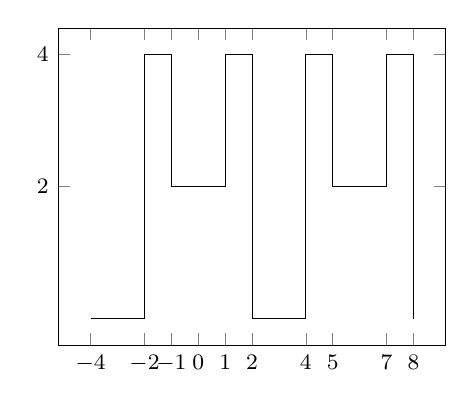
\begin{tikzpicture}
\begin{axis}[small,xtick={-4,-2,-1,0,1,2,4,5,7,8},xticklabels={$-4$,$-2$,$-1$,$0$,$1$,$2$,$4$,$5$,$7$,$8$},ytick={2,4},yticklabels={$2$,$4$}]
\addplot[] plot coordinates { (-4,0) (-2,0) (-2,4) (-1,4) (-1,2) (1,2) (1,4) (2,4) (2,0) (4,0) (4,4) (5,4) (5,2) (7,2) (7,4) (8,4) (8,0)};
\end{axis}
\end{tikzpicture}
\caption*{(الف)}
\end{subfigure}%
\begin{subfigure}{0.5\textwidth}
\centering
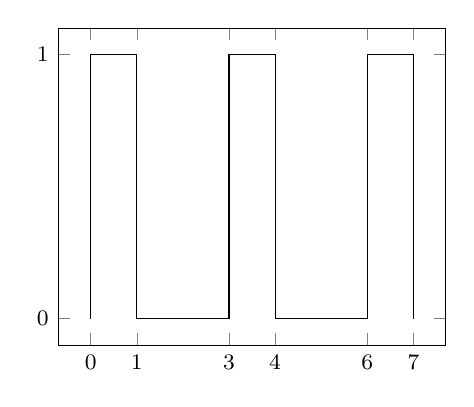
\begin{tikzpicture}
\begin{axis}[small,xtick={0,1,3,4,6,7},xticklabels={$0$,$1$,$3$,$4$,$6$,$7$},ytick={0,1},yticklabels={$0$,$1$}]
\addplot[] plot coordinates { (0,0) (0,1) (1,1) (1,0) (3,0) (3,1) (4,1) (4,0) (6,0) (6,1) (7,1) (7,0) };
\end{axis}
\end{tikzpicture}
\caption*{(ب)}
\end{subfigure}%
\caption{مشق \حوالہ{مشق_فوریئر_جفت_تفاعل_قوت_نمائی_تسلسل_الف} اور مشق \حوالہ{مشق_فوریئر_جفت_تفاعل_قوت_نمائی_تسلسل_ب} کے تفاعل۔}
\label{شکل_فوریئر_جفت_تفاعل_قوت_نمائی_تسلسل_الف}
\end{figure}

جوابات:
\begin{align*}
\kx{c}_0&=\frac{1}{2}\\
\kx{c}_n&=\frac{2}{n\pi}\left[2\sin \frac{2\pi n}{3}-\sin\frac{n\pi}{3}\right]
\end{align*}
\انتہا{مشق}
%================

\ابتدا{مشق}\شناخت{مشق_فوریئر_جفت_تفاعل_قوت_نمائی_تسلسل_ب}
شکل \حوالہ{شکل_فوریئر_جفت_تفاعل_قوت_نمائی_تسلسل_الف}-ب میں دیے تفاعل کے قوت نمائی فوریئر تسلسل کے عددی سر معلوم کریں۔

جوابات:
\begin{align*}
\kx{c}_0&=\frac{1}{3}\\
\kx{c}_n&=\frac{1-e^{-j\frac{2}{3}n\pi}}{j2n\pi}
\end{align*}
\انتہا{مشق}
%======================================================================
\حصہ{تشاکل تفاعل}
آپ نے مختلف تفاعل کے فوریئر تسلسل دیکھے۔ان میں کئی ایسے تھے جن کے یا تمام \عددی{a_m} اور یا تمام \عددی{b_m} صفر کے برابر تھے۔آئیں اس کی وجہ سمجھیں اور تکملات حل کرنے سے پہلے یہ دریافت کرنا سیکھیں کہ آیا فوریئر تسلسل میں \عددی{a_m} اور یا تمام \عددی{b_m} صفر کے برابر ہوں گے۔فوریئر تسلسل کے ارکان کا دارومدار تفاعل کی شکل و صورت پر ہے۔ تین قسم کے تشاکل تفاعل پائے جاتے ہیں۔ان پر باری باری غور کرتے ہیں۔

\جزوحصہ{جفت تشاکل تفاعل}
جفت تفاعل سے مراد ایسا تفاعل ہے جو درج ذیل مساوات پر پورا اترتا ہو۔
\begin{align}
f(t)=f(-t)
\end{align}
جفت  تفاعل عمودی محور کے دونوں اطراف یکساں دکھائی دیتا ہے۔جفت تفاعل کی اہم مثال \عددی{\cos(n\omega_0 t)} ہے۔آپ جانتے ہیں کہ \عددی{\cos(\theta)=\cos(-\theta)} ہوتا ہے لہٰذا یہ جفت تفاعل ہے۔شکل \حوالہ{شکل_فوریئر_مستطیل_موج_الف}-الف بھی جفت تفاعل ہے۔ آئیں جفت تفاعل کے فوریئر تسلسل کے عددی سر حاصل کریں۔

مساوات \حوالہ{مساوات_فوریئر_عددی_سر_ت} میں تکمل کو \عددی{-\tfrac{T_0}{2}\le  t \le \tfrac{T_0}{2}} لیتے ہوئے یہاں دوبارہ پیش کرتے ہیں۔
\begin{gather}
\begin{aligned}\label{مساوات_فوریئر_عددی_سر_جفت}
a_0&=\frac{1}{T_0}\int_{-\frac{T_0}{2}}^{\frac{T_0}{2}}f(t) \dif t\\
a_m&=\frac{2}{T_0}\int_{-\frac{T_0}{2}}^{\frac{T_0}{2}}f(t) \cos (m \omega_0 t) \dif t\\
b_m&=\frac{2}{T_0}\int_{-\frac{T_0}{2}}^{\frac{T_0}{2}}f(t) \sin (m \omega_0 t) \dif t
\end{aligned}
\end{gather}
\عددی{a_0} کی مساوات کو درج ذیل لکھا جا سکتا ہے۔
\begin{align*}
a_0&=\frac{1}{T_0}\int_{-\frac{T_0}{2}}^0 f(t) \dif t+\frac{1}{T_0}\int_0^{\frac{T_0}{2}} f(t) \dif t
\end{align*}
ان میں پہلے تکمل میں متغیرہ کو تبدیل کرتے ہوئے \عددی{t=-x} لکھنے سے \عددی{f(t)=f(-x)} اور \عددی{\dif t=-\dif x} لکھے جائیں گے اور تکمل کے حدود \عددی{\tfrac{T_0}{2} \le t \le 0} ہوں گے۔چونکہ تفاعل جفت ہے لہٰذا \عددی{f(-x)=f(x)} ہو گا۔یوں درج ذیل لکھا جا سکتا ہے
\begin{gather}
\begin{aligned}
a_0&=-\frac{1}{T_0}\int_{\frac{T_0}{2}}^0 f(-x) \dif x+\frac{1}{T_0}\int_0^{\frac{T_0}{2}} f(t) \dif t\\
&=\frac{1}{T_0}\int_0^{\frac{T_0}{2}} f(x) \dif x+\frac{1}{T_0}\int_0^{\frac{T_0}{2}} f(t) \dif t\\
&=\frac{2}{T_0}\int_0^{\frac{T_0}{2}} f(t) \dif t
\end{aligned}
\end{gather}
جہاں آخری قدم پر دونوں تکمل میں صرف متغیرات کی علامت مختلف ہے لہٰذا ان کی قیمتیں برابر ہیں۔

\عددی{a_m} کو بھی اسی طرح حاصل کرتے ہیں۔
\begin{gather}
\begin{aligned}
a_m&=\frac{2}{T_0}\int_{-\frac{T_0}{2}}^{0}f(t) \cos (m \omega_0 t) \dif t+\frac{2}{T_0}\int_{0}^{\frac{T_0}{2}}f(t) \cos (m \omega_0 t) \dif t\\
&=-\frac{2}{T_0}\int_{\frac{T_0}{2}}^{0}f(-x) \cos (-m \omega_0 x) \dif x+\frac{2}{T_0}\int_{0}^{\frac{T_0}{2}}f(t) \cos (m \omega_0 t) \dif t\\
&=\frac{2}{T_0}\int_0^{\frac{T_0}{2}}f(x) \cos (m \omega_0 x) \dif x+\frac{2}{T_0}\int_{0}^{\frac{T_0}{2}}f(t) \cos (m \omega_0 t) \dif t\\
&=\frac{4}{T_0}\int_{0}^{\frac{T_0}{2}}f(t) \cos (m \omega_0 t) \dif t
\end{aligned}
\end{gather}
آخر میں \عددی{b_m} کو اسی ترکیب سے حاصل کرتے ہیں
\begin{gather}
\begin{aligned}
b_m&=\frac{2}{T_0}\int_{-\frac{T_0}{2}}^{0}f(t) \sin (m \omega_0 t) \dif t+\frac{2}{T_0}\int_{0}^{\frac{T_0}{2}}f(t) \sin (m \omega_0 t) \dif t\\
&=-\frac{2}{T_0}\int_{\frac{T_0}{2}}^{0}f(-x) \sin(-m \omega_0 x) \dif x+\frac{2}{T_0}\int_{0}^{\frac{T_0}{2}}f(t) \sin (m \omega_0 t) \dif t\\
&=\frac{2}{T_0}\int_0^{\frac{T_0}{2}}f(x) \sin (-m \omega_0 x) \dif x+\frac{2}{T_0}\int_{0}^{\frac{T_0}{2}}f(t) \cos (m \omega_0 t) \dif t\\
&=0
\end{aligned}
\end{gather}
جہاں آخری قدم پر \عددی{\sin(-m\omega_0 t)=-\sin(m\omega_0 t)} کا استعمال کیا گیا ہے۔

آپ نے دیکھا کہ جفت تفاعل کی صورت میں فوریئر تسلسل کے \عددی{b_m=0} ہیں لہٰذا انہیں حاصل کرنے کی ضرورت نہیں ہے۔
%================================
\جزوحصہ{طاق تشاکل تفاعل}
طاق تفاعل سے مراد ایسا تفاعل ہے جو درج ذیل مساوات پر پورا اترتا ہو۔
\begin{align}
f(-t)=-f(t)
\end{align}
طاق تفاعل کی مثال \عددی{\sin(m\omega_0 t)} ہے۔ہم جفت تفاعل کی طرح طاق تفاعل کے عددی سر حاصل کرتے ہوئے درج ذیل نتائج پر پہنچتے ہیں۔
\begin{gather}
\begin{aligned}
a_0&=0\\
a_m&=0\\
b_m&=\frac{4}{T_0}\int_{0}^{\frac{T_0}{2}}f(t) \sin (m \omega_0 t) \dif t
\end{aligned}
\end{gather}
یوں طاق تفاعل کے فوریئر تسلسل کے صرف \عددی{b_m} عددی سر حاصل کرنے کی ضرورت پیش آئے گی۔
%=================================

\ابتدا{مثال}\شناخت{مثال_فوریئر_جفت_مستطیل}
شکل \حوالہ{شکل_فوریئر_جفت_طاق_مستطیل}-الف میں جفت تفاعل دکھایا گیا ہے۔اس کے فوریئر تکونیاتی تسلسل کے عددی سر حاصل کریں۔
\begin{figure}
\centering
\begin{subfigure}{0.5\textwidth}
\centering
\begin{tikzpicture}
\begin{axis}[small,xtick={-1,0,1,3,5},xticklabels={$-1$,$0$,$1$,$3$,$5$},ytick={0,1},yticklabels={$0$,$1$}]
\addplot[] plot coordinates {(-1,0) (-1,1) (1,1) (1,0) (3,0) (3,1) (5,1) (5,0)};
\end{axis}
\end{tikzpicture}
\caption*{(الف)}
\end{subfigure}%
\begin{subfigure}{0.5\textwidth}
\centering
\begin{tikzpicture}
\begin{axis}[small,xtick={0,2,4,6},xticklabels={$0$,$2$,$4$,$6$},ytick={0,1},yticklabels={$0$,$1$}]
\addplot[] plot coordinates {(0,0) (0,1) (2,1) (2,0) (4,0) (4,1) (6,1) (6,0)};
\end{axis}
\end{tikzpicture}
\caption*{(ب)}
\end{subfigure}%
\caption{مثال \حوالہ{مثال_فوریئر_جفت_مستطیل} اور مثال \حوالہ{مثال_فوریئر_طاق_مستطیل} کے اشکال۔}
\label{شکل_فوریئر_جفت_طاق_مستطیل}
\end{figure}

حل:چونکہ دیا تفاعل جفت ہے لہٰذا \عددی{b_m=0} ہوں گے۔بقایا عددی سر دریافت کرتے ہیں یعنی
\begin{align*}
a_0&=\frac{1}{4}\int_{-1}{1} \dif t\\
&=\frac{1}{2}
\end{align*}
اور
\begin{align*}
a_n&=\frac{2}{4}\int_{-1}^{1} \cos (n\omega_0 t) \dif t\\
&=\frac{\sin \frac{n\pi}{2}}{\frac{n\pi}{2}}
\end{align*}
\انتہا{مثال}
%=================================

\ابتدا{مثال}\شناخت{مثال_فوریئر_طاق_مستطیل}
شکل \حوالہ{شکل_فوریئر_جفت_طاق_مستطیل}-ب میں طاق تفاعل دکھایا گیا ہے۔اس کے فوریئر تکونیاتی تسلسل کے عددی سر حاصل کریں۔

حل:چونکہ دیا تفاعل طاق ہے لہٰذا \عددی{a_m=0} ہوں گے۔بقایا عددی سر دریافت کرتے ہیں یعنی
\begin{align*}
a_0&=\frac{1}{4}\int_{0}{2} \dif t\\
&=\frac{1}{2}
\end{align*}
اور
\begin{align*}
b_n&=\frac{2}{4}\int_{0}^{2} \sin (n\omega_0 t) \dif t\\
&=\frac{1-\cos n\pi}{n\pi}
\end{align*}
\انتہا{مثال}
%=================================

\حصہ{منتقلی وقت}
فرض کریں کہ ایک تفاعل جس کی فوریئر تسلسل درج ذیل ہے
\begin{align}
f(t)=\sum_{n=-\infty}^{\infty} \kx{c}_n e^{jn\omega_0 t}
\end{align}
کو وقت کے لحاض سے منتقل کیا جاتا ہے۔تفاعل \عددی{f(t)} کو \عددی{t_0} سیکنڈ تاخیر سے  \عددی{f(t-t_0)} لکھا جاتا ہے۔
\begin{gather}
\begin{aligned}\label{مساوات_فوریئر_تبادلہ_وقت}
f(t-t_0)&=\sum_{n=-\infty}^{\infty} \kx{c}_n e^{jn\omega_0 (t-t_0)}\\
&=\sum_{n=-\infty}^{\infty} \left(\kx{c}_n e^{-jn\omega_0 t_0}\right) e^{jn\omega_0 t}
\end{aligned}
\end{gather}
چونکہ \عددی{e^{-jn\omega_0 t_0}} سے مراد زاویائی فاصلہ ہے لہٰذا وقت میں منتقل تفاعل \عددی{f(t-t_0)} کے فوریئر عددی سر اصل تفاعل \عددی{f(t)} کے عددی سر ہوتے ہیں جن میں تعدد کے راست متناسب زاویائی ہٹاو \عددی{e^{-jn\omega_0 t_0}}  پایا جاتا ہے۔ اس طرح وقتی دائرہ کار میں تبادلے سے  تعددی دائرہ کار میں مراد  زاویائی تبادلہ ہے۔

%============
\ابتدا{مثال}\شناخت{مثال_فوریئر_دندان_منتقل_دوبارہ}
مثال \حوالہ{مثال_فوریئر_دندان_دوبارہ} میں ہم شکل \حوالہ{شکل_فوریئر_دندان_دوبارہ} کے تفاعل \عددی{f(t)} کا قوت نمائی فوریئر تسلسل حاصل کر چکے ہیں۔ اس تفاعل کو \عددی{\tfrac{T}{4}} بائیں منتقل کرتے ہوئے شکل \حوالہ{شکل_فوریئر_دندان_منتقل_دوبارہ} یعنی \عددی{f(t+\tfrac{T}{4})} حاصل ہوتا ہے جس کی قوت نمائی فوریئر تسلسل درکار ہے۔
\begin{figure}
\centering
\begin{tikzpicture}
\begin{axis}[small,xlabel={$t$},ylabel style={rotate=-90},xtick={-0.5,0,0.5,1.5},xticklabels={$-\frac{T}{4}$,$0$,$\frac{T}{4}$,$\frac{3T}{4}$},ytick={-1,0,1},yticklabels={$-V_0$,$0$,$V_0$}]
\addplot[] plot coordinates{(-0.75,-1) (-0.5,-1) (-0.5,1) (0.5,1) (0.5,-1) (1.5,-1) (1.5,1) (2.5,1) (2.5,-1) (2.75,-1)};
\end{axis}
\end{tikzpicture}
\caption{مثال \حوالہ{مثال_فوریئر_دندان_منتقل_دوبارہ} کا تفاعل۔}
\label{شکل_فوریئر_دندان_منتقل_دوبارہ}
\end{figure}%
حل: اس کو تبادلہ وقت کے کلیے سے حل کرتے ہیں۔مساوات \حوالہ{مساوات_فوریئر_تبادلہ_وقت} کے ذریعہ نئے عددی سر حاصل کرتے ہیں۔چونکہ \عددی{t_0=-\tfrac{T}{4}} ہے لہٰذا زاویائی ہٹاو
\begin{align*}
-jn\omega_0 t_0=jn \frac{2\pi}{T} \frac{T}{4}=jn\frac{\pi}{2}
\end{align*}
ہو گا۔یوں بنیادی ہارمونی رکن کے عددی سر میں \عددی{90^{\circ}} کا زاویائی ہٹاو پایا جائے گا۔ مساوات \حوالہ{مساوات_فوریئر_مستطیل_دوسرا_جواب} میں ان زاویائی ہٹاو کو شامل کرتے ہوئے فوریئر تسلسل لکھتے ہیں۔
\begin{align}
f\left(t+\frac{T}{4}\right)&=\sum_{\substack{n=-\infty \\ n=\text{طاق}\\ n \ne 0} }^{\infty} -\frac{j2V_0}{n\pi}e^{jn\left(\omega_0 +\frac{\pi}{2}\right)t}
\end{align}
\انتہا{مثال}
%============

\حصہ{تخلیق موج}
دو یا دو سے زیادہ امواج کا مجموعہ لیتے ہوئے دیگر امواج حاصل کئے جا سکتے ہیں۔یوں شکل \حوالہ{شکل_فوریئر_تخلیق_موج}-الف اور شکل-ب مل کر شکل-پ دیتے ہیں۔انفرادی امواج کے فوریئر تسلسل کا مجموعہ حاصل موج کی فوریئر تسلسل دے گی۔ فوریئر تسلسل میں تعددی ارکان کا دارومدار وقت کے لحاض سے موج کی صورت پر منحصر ہوتا ہے نا کہ موج کی حتمی قیمت پر۔یوں جس نسبت سے موج کا حیطہ تبدیل کیا جائے اسی نسبت سے تسلسل کو ضرب دیتے ہوئے کم یا زیادہ حیطے کی موج کا تسلسل حاصل کیا جا سکتا ہے۔ 
\begin{figure}
\centering
\begin{subfigure}{0.5\textwidth}
\centering
\begin{tikzpicture}
\begin{axis}[small,ytick={0,1},yticklabels={$0$,$1$},xtick={-2,0,2,4,8},xticklabels={$-2$,$0$,$2$,$4$,$8$},ymax=2.2,xmin=-2.5,xmax=8.5]
\addplot[] plot coordinates {(-2.5,0)(-2,0) (-2,1) (2,1) (2,0) (4,0) (4,1) (8,1) (8,0)(8.5,0)};
\end{axis}
\end{tikzpicture}
\caption*{(الف)}
\end{subfigure}%
\begin{subfigure}{0.5\textwidth}
\centering
\begin{tikzpicture}
\begin{axis}[small,ytick={0,1},yticklabels={$0$,$1$},xtick={-1,0,1,5,7},xticklabels={$-1$,$0$,$1$,$5$,$7$},ymax=2.2,xmin=-2.5,xmax=8.5]
\addplot[] plot coordinates {(-2.5,0)(-1,0) (-1,1) (1,1) (1,0) (5,0) (5,1) (7,1) (7,0) (8.5,0)};
\end{axis}
\end{tikzpicture}
\caption*{(ب)}
\end{subfigure}
\begin{subfigure}{0.5\textwidth}
\centering
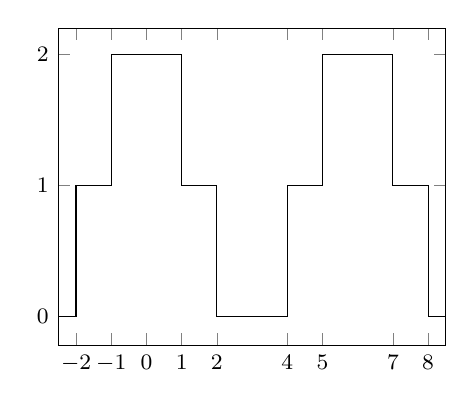
\begin{tikzpicture}
\begin{axis}[small,ytick={0,1,2},yticklabels={$0$,$1$,$2$},xtick={-2,-1,0,1,2,4,5,7,8},xticklabels={$-2$,$-1$,$0$,$1$,$2$,$4$,$5$,$7$,$8$},ymax=2.2,xmin=-2.5,xmax=8.5]
\addplot[] plot coordinates {(-2.5,0)(-2,0) (-2,1) (-1,1) (-1,2) (1,2) (1,1) (2,1) (2,0) (4,0) (4,1) (5,1) (5,2) (7,2) (7,1) (8,1) (8,0)(8.5,0)};
\end{axis}
\end{tikzpicture}
\caption*{(پ)}
\end{subfigure}
\caption{دو یا دو سے زیادہ امواج کے جمع و منفی سے نئی موج کی تخلیق۔}
\label{شکل_فوریئر_تخلیق_موج}
\end{figure}

فوریئر تسلسل میں \عددی{\sum a_n \cos (n\omega_0 t)} جفت موج کو ظاہر کرتی ہے جبکہ \عددی{\sum b_n \sin(n\omega_0 t)} طاق موج کو ظاہر کرتی ہے لہٰذا کسی بھی موج کو جفت موج اور طاق موج کا مجموعہ تصور کیا جا سکتا ہے۔
%================

\ابتدا{مشق}
شکل \حوالہ{شکل_فوریئر_تخلیق_موج}-الف اور ب کی فوریئر قوت نمائی تسلسل کے عددی سر حاصل کریں۔ان کے مجموعے سے شکل-پ کی تسلسل کے عددی سر حاصل کریں۔

جواب:\عددی{\kx{c}_0=1}، \عددی{\kx{c}_n=\tfrac{\sin\tfrac{2n\pi}{3}+\sin\tfrac{n\pi}{3}}{n\pi}}
\انتہا{مشق}
%======================
\ابتدا{مشق}\شناخت{مشق_تخلیق_موج_ب}
شکل \حوالہ{شکل_تخلیق_موج_ب}-ال اور ب کا مجموعہ شکل-پ ہے۔شکل-الف اور ب کے فوریئر تسلسل حاصل کرتے ہوئے شکل-پ کا تسلسل حاصل کریں۔
\begin{figure}
\centering
\begin{subfigure}{0.5\textwidth}
\centering
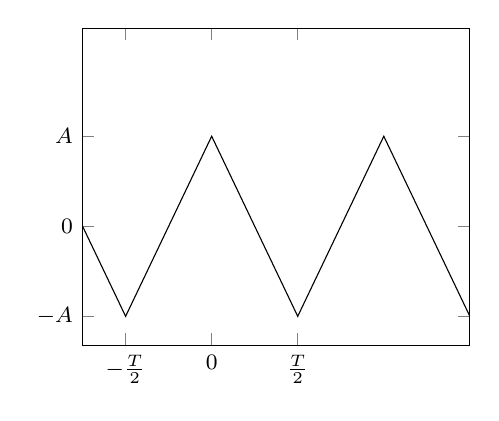
\begin{tikzpicture}
\begin{axis}[small,ytick={-1,0,1},yticklabels={$-A$,$0$,$A$},xtick={-1,0,1},xticklabels={$-\frac{T}{2}$,$0$,$\frac{T}{2}$},ymax=2.2,xmin=-1.5,xmax=3]
\addplot[] plot coordinates {(-1.5,0)(-1,-1) (0,1) (1,-1) (2,1) (3,-1)};
\end{axis}
\end{tikzpicture}
\caption*{(الف)}
\end{subfigure}%
\begin{subfigure}{0.5\textwidth}
\centering
\begin{tikzpicture}
\begin{axis}[small,ytick={-1,0,1},yticklabels={$-A$,$0$,$A$},xtick={-1,0,1},xticklabels={$-\frac{T}{2}$,$0$,$\frac{T}{2}$},ymax=2.2,xmin=-1.5,xmax=3]
\addplot[] plot coordinates {(-1.5,-1) (-1,-1) (-1,1) (0,1) (0,-1) (1,-1) (1,1) (2,1) (2,-1) (3,-1)};
\end{axis}
\end{tikzpicture}
\caption*{(ب)}
\end{subfigure}
\begin{subfigure}{0.5\textwidth}
\centering
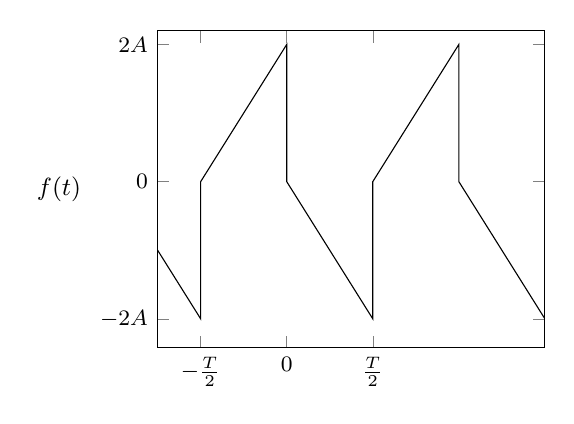
\begin{tikzpicture}
\begin{axis}[small,ylabel={$f(t)$},ylabel style ={rotate=-90},ytick={-2,0,2},yticklabels={$-2A$,$0$,$2A$},xtick={-1,0,1},xticklabels={$-\frac{T}{2}$,$0$,$\frac{T}{2}$},ymax=2.2,xmin=-1.5,xmax=3]
\addplot[] plot coordinates {(-1.5,-1)(-1,-2)(-1,0)(0,2) (0,0) (1,-2) (1,0) (2,2) (2,0) (3,-2)};
\end{axis}
\end{tikzpicture}
\caption*{(پ)}
\end{subfigure}
\caption{مشق \حوالہ{مشق_تخلیق_موج_ب} کے اشکال۔}
\label{شکل_تخلیق_موج_ب}
\end{figure}

جواب:
$f(t)=\sum_{\substack{n=1 \\ \text{طاق}}}^{\infty} \left[\frac{4A}{n\pi}\sin(n\omega_0 t)-\frac{8A}{n^2\pi^2} \cos(n\omega_0 t)\right]$
\انتہا{مشق}
%==========================
\حصہ{تعددی طیف}
تفاعل \عددی{f(t)} کے عددی سر کی مقدار بالمقابل تعدد کے ترسیم کو \اصطلاح{مقداری طیف}\فرہنگ{مقداری!طیف}\فرہنگ{طیف!مقداری}\حاشیہب{amplitude spectrum}\فرہنگ{spectrum!amplitude}\فرہنگ{amplitude!spectrum} کہتے ہیں جبکہ عددی سر کی زاویائی ہٹاو بالمقابل تعدد کے ترسیم کو \اصطلاح{زاویائی ہٹاو طیف}\فرہنگ{زاویائی ہٹاو!طیف}\فرہنگ{طیف!زاویائی ہٹاو}\حاشیہب{phase spectrum}\فرہنگ{phase!spectrum}\فرہنگ{spectrum!phase} کہتے ہیں۔ چونکہ طیف انفرادی لکیروں پر مشتمل ہے لہٰذا اسے \اصطلاح{انفرادی لکیری طیف}\فرہنگ{انفرادی لکیری طیف}\فرہنگ{طیف!انفرادی لکیری}\حاشیہب{discrete line spectra}\فرہنگ{discrete line spectra}
\فرہنگ{spectrum!discrete line} کہتے ہیں۔انفرادی لکیری طیف تفاعل کی تعددی مواد کے بارے میں معلومات دیتی ہے۔

%=====================
\ابتدا{مثال}\شناخت{مثال_فوریئر_طیف_دیا_گیا_ہے}
مشق \حوالہ{مشق_تخلیق_موج_ب} میں شکل \حوالہ{شکل_تخلیق_موج_ب}-پ کا تسلسل حاصل کیا گیا جو \عددی{A=5} کی صورت میں درج ذیل ہو گا۔
\begin{align*}
f(t)=\sum_{\substack{n=1 \\ \text{طاق}}}^{\infty} \left[\frac{20}{n\pi}\sin(n\omega_0 t)-\frac{40}{n^2\pi^2} \cos(n\omega_0 t)\right]
\end{align*}
تفاعل کی مقداری طیف اور زاویائی ہٹاو طیف درکار ہے۔

حل:چونکہ \عددی{D_n\phase{\theta_n}=a_n-jb_n} ہے لہٰذا پہلے چار \عددی{D_n\phase{\theta_n}} درج ذیل ہوں گے۔
\begin{align*}
D_1\phase{\theta_1}&=-\frac{40}{\pi^2}-j\frac{20}{\pi}=7.5\phase{-122^{\circ}}\\
D_3\phase{\theta_1}&=-\frac{40}{9\pi^2}-j\frac{20}{3\pi}=2.2\phase{-102^{\circ}}\\
D_5\phase{\theta_1}&=-\frac{40}{25\pi^2}-j\frac{20}{5\pi}=1.3\phase{-97^{\circ}}\\
D_7\phase{\theta_1}&=-\frac{40}{49\pi^2}-j\frac{20}{7\pi}=0.91\phase{-95^{\circ}}\\
\end{align*}
مقداری طیف اور زاویائی ہٹاو طیف کو شکل \حوالہ{شکل_فوریئر_طیف_دیا_گیا_ہے} میں دکھایا گیا ہے۔
\begin{figure}
\centering
\begin{subfigure}{0.5\textwidth}
\centering
\begin{tikzpicture}
\begin{axis}[small,axis lines*=middle,ylabel={$D_n$},ylabel style={rotate=-90},xlabel={$\omega_0$},xtick={1,3,5,7},xticklabels={$\omega_0$,$3\omega_0$,$5\omega_0$,$7\omega_0$},ytick={1,2,3,4,5,6,7,8},yticklabels={$1$,$2$,$3$,$4$,$5$,$6$,$7$,$8$},ymin=0,y label style={at={(axis description cs:0,1.1)}}]
\addplot[] plot coordinates {(1,0) (1,7.5)};
\addplot[] plot coordinates {(3,0) (3,2.2)};
\addplot[] plot coordinates {(5,0) (5,1.3)};
\addplot[] plot coordinates {(7,0) (7,0.91)};
\end{axis}
\end{tikzpicture}
\caption*{(الف) مقداری طیف۔}
\end{subfigure}%
\begin{subfigure}{0.5\textwidth}
\centering
\begin{tikzpicture}
\begin{axis}[small,axis lines*=middle,ylabel={$\theta_n$},ylabel style={rotate=-90},xlabel={$\omega_0$},xtick={1,3,5,7},xticklabels={$\omega_0$,$3\omega_0$,$5\omega_0$,$7\omega_0$},ytick={-20,-40,-60,-80,-100,-120,-140},yticklabels={$-20^{\circ}$,$-40^{\circ}$,$-60^{\circ}$,$-80^{\circ}$,$-100^{\circ}$,$-120^{\circ}$,$-140^{\circ}$},ymax=20 ,x tick label style={above},x label style={at={(axis description cs:0.5,1.2)}},x tick style={draw=none},y label style={at={(axis description cs:0,1.05)}}]
\addplot[] plot coordinates {(1,0) (1,-122)};
\addplot[] plot coordinates {(3,0) (3,-102)};
\addplot[] plot coordinates {(5,0) (5,-97)};
\addplot[] plot coordinates {(7,0) (7,-95)};
\end{axis}
\end{tikzpicture}
\caption*{(ب) زاویائی ہٹاو طیف۔}
\end{subfigure}
\caption{مثال \حوالہ{مثال_فوریئر_طیف_دیا_گیا_ہے} کے طیف۔}
\label{شکل_فوریئر_طیف_دیا_گیا_ہے}
\end{figure}
\انتہا{مثال}
%==================
\ابتدا{مشق}\شناخت{مشق_فوریئر_طیف_الف}
شکل \حوالہ{شکل_فوریئر_طیف_الف} میں دیے تفاعل کے \عددی{D_n} عددی سر حاصل کریں۔
\begin{figure}
\centering
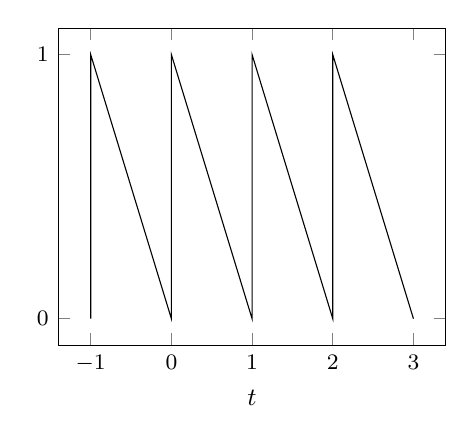
\begin{tikzpicture}
\begin{axis}[small,xlabel={$t$},ylabel style={rotate=-90},xtick={-1,0,1,2,3},xticklabels={$-1$,$0$,$1$,$2$,$3$},ytick={0,1},yticklabels={$0$,$1$}]
\addplot[] plot coordinates {(-1,0) (-1,1) (0,0) (0,1) (1,0) (1,1) (2,0) (2,1) (3,0)};
\end{axis}
\end{tikzpicture}
\caption{مشق \حوالہ{مشق_فوریئر_طیف_الف} کا تفاعل۔}
\label{شکل_فوریئر_طیف_الف}
\end{figure}
جوابات:
\begin{align*}
a_0&=\frac{1}{2}\\
D_1&=-\frac{j}{\pi}\\
D_2&=-\frac{j}{2\pi}\\
D_3&=-\frac{j}{3\pi}\\
D_4&=-\frac{j}{4\pi}
\end{align*}
\انتہا{مشق}
%==================
\ابتدا{مشق}\شناخت{مشق_فوریئر_طیف_دیا_گیا}
انفرادی لکیری طیف شکل \حوالہ{شکل_فوریئر_طیف_دیا_گیا} میں دکھائے گئے ہیں۔تفاعل کی تکونیاتی تسلسل لکھیں۔
\begin{figure}
\centering
\begin{subfigure}{0.5\textwidth}
\centering
\begin{tikzpicture}
\begin{axis}[small,ylabel={$D_n$},ylabel style={rotate=-90},xlabel={$f\,(\si{\hertz})$},xtick={0,20,40,60,80},xticklabels={$0$,$20$,$40$,$60$,$80$},ytick=\empty,,ymin=0,ymax=1.7,y label style={at={(axis description cs:0,1.1)}}]
\addplot[] plot coordinates {(0,0) (0,0.25)}node[circ]{}node[above]{$0.25$};
\addplot[] plot coordinates {(20,0) (20,1.35)}node[circ]{}node[above]{$1.35$};
\addplot[] plot coordinates {(40,0) (40,1)}node[circ]{}node[above]{$1$};
\addplot[] plot coordinates {(60,0) (60,0.5)}node[circ]{}node[above]{$0.5$};
\addplot[] plot coordinates {(80,0) (80,0.35)}node[circ]{}node[above]{$0.35$};
\end{axis}
\end{tikzpicture}
\caption*{(الف) مقداری طیف۔}
\end{subfigure}%
\begin{subfigure}{0.5\textwidth}
\centering
\begin{tikzpicture}
\begin{axis}[small,axis lines*=middle,ylabel={$\theta_n$},ylabel style={rotate=-90},xlabel={$f\,(\si{\hertz})$},xtick={0,20,40,60,80},xticklabels={$0$,$20$,$40$,$60$,$80$},ytick={-45,-90,-135},yticklabels={$-45^{\circ}$,$-90^{\circ}$,$-135^{\circ}$},ymax=20 ,x tick label style={above},x label style={at={(axis description cs:0.5,1.2)}},x tick style={draw=none},y label style={at={(axis description cs:0,1.05)}}]
\addplot[] plot coordinates {(20,0) (20,-135)};
\addplot[] plot coordinates {(40,0) (40,-90)};
\addplot[] plot coordinates {(60,0) (60,-45)};
\addplot[] plot coordinates {(80,0) (80,-135)};
\end{axis}
\end{tikzpicture}
\caption*{(ب) زاویائی ہٹاو طیف۔}
\end{subfigure}
\caption{مشق \حوالہ{مشق_فوریئر_طیف_دیا_گیا} کے طیف۔}
\label{شکل_فوریئر_طیف_دیا_گیا}
\end{figure}

جواب:
 \begin{multline*}
f(t)=0.25+1.35\cos(40\pi t-135^{\circ})+1\cos(80\pi t-90^{\circ})\\
+0.5\cos(120\pi t-45^{\circ})+0.35\cos(160\pi t-135^{\circ})+\cdots
\end{multline*}
\انتہا{مشق}
%===================

\حصہ{برقرار حال برقی جال}
کسی دور پر سائن نما دباو مسلط کرتے ہوئے دور میں مختلف مقامات پر دباو اور رو حاصل کرنا ہم دیکھ چکے ہیں۔فرض کریں کہ کسی دور پر  دوری دباو \عددی{v(t)} مسلط کی جاتی ہے۔ایسے دور کو حل کرنے  کی خاطر ہم مسلط دباو کا فوریئر تسلسل حاصل کرتے ہیں۔فوریئر تسلسل کا ہر رکن سائن نما دباو ہو گا۔انفرادی ہارمونی دباو کے لئے دور کو تعددی دائرہ کار میں حل کیا جاتا ہے۔ ان جوابات کا وقتی دائرہ کار میں مطلوبہ قیمت حاصل کی جاتی ہے۔تمام جوابات کا مجموعہ درکار جواب ہوتا ہے۔

\جزوحصہ{اوسط طاقت}
جیسا اوپر ذکر کیا گیا، دور پر دوری دباو یا دوری رو مسلط کرنے سے مختلف مقامات پر دباو اور رو پیدا ہوں گے جنہیں تسلسل کی صورت میں درج ذیل لکھا جا سکتا ہے۔ 
\begin{align}
v(t)&=V_{DC}+\sum_{n=1}^{\infty} V_n \cos (n\omega_0 t-\theta_{v,n})\\
i(t)&=I_{DC}+\sum_{n=1}^{\infty} I_n \cos (n\omega_0 t-\theta_{i,n})
\end{align}
غیر فعال رائج سمت استعمال کرتے ہوئے فرض کریں کہ کسی پرزے پر دباو اور اس میں رو درج بالا مساوات دیتے ہیں۔یوں اس پرزے کی اوسط طاقت درج ذیل ہو گی۔
\begin{align}\label{مساوات_فوریئر_طاقت_الف}
P&=\frac{1}{T}\int_0^T v(t)i(t) \dif t
\end{align}
درج بالا مساوات میں دو فوریئر تسلسل کے حاصل ضرب کا تکمل لیا گیا ہے۔ دو عدد فوریئر تسلسل کے حاصل ضرب  میں تین قسم کے ارکان پائے جاتے ہیں۔ایک رکن \عددی{V_{DC}I_{DC}} ہے جس کا تکمل تقسیم \عددی{T} از خود \عددی{V_{DC}I_{DC}} کے برابر ہے۔ دوسرا قسم وہ ہے جو \عددی{V_{DC} I_n\cos(n\omega_0 t -\theta_{i,n})} یا \عددی{I_{DC} V_n\cos(n\omega_0 t -\theta_{v,n})} صورت رکھتے ہیں۔ آپ جانتے ہیں کہ سائن نما تفاعل کا ایک دوری عرصے پر تکمل صفر کے برابر ہوتا ہے لہٰذا ایسے تمام ارکان صفر کے برابر ہوں گے۔تیسرا اور سب سے زیادہ تعداد میں  ارکان \عددی{\cos(m\omega_0 t -\theta_{v,n}) \cos(n\omega_0 t-\theta_{i,n})} صورت رکھتے ہیں۔آپ جانتے ہیں کہ \عددی{\cos(n\omega_0 t)} اور \عددی{\sin(n\omega_0 t)} آپس میں عمودی تفاعل ہیں لہٰذا \عددی{m \ne n} کی صورت میں تمام 
 \عددی{\cos(m\omega_0 t -\theta_{v,n}) \cos(n\omega_0 t-\theta_{i,n})} کا ایک دوری عرصے پر تکمل صفر کے برابر ہو گا۔یوں صرف ایسے ارکان غیر صفر ہوں گے جن میں دباو کی تعدد  اور رو کی تعدد برابر ہو یعنی
\begin{align*}
\sum_{n=1}^{\infty} \frac{1}{T}\int_0^T V_n I_n \cos(n\omega_0 t-\theta_{v,n})\cos(n\omega_0 t-\theta_{i,n}) \dif t=\sum_{n=1}^{\infty} \frac{V_n I_n}{2} \cos(\theta_{v,n}-\theta_{i,n})
\end{align*}
اس طرح اوسط طاقت درج ذیل ہو گی۔
\begin{align}
P=V_{DC}I_{DC}+\sum_{n=1}^{\infty}\frac{ V_n I_n}{2} \cos(\theta_{v,n}-\theta_{i,n})
\end{align}
درج بالا مساوات کا مطلب ہے کہ تمام انفرادی ہارمونی اجزاء کے اوسط طاقت کا مجموعہ کل اوسط طاقت دیتا ہے۔
%====================
\ابتدا{مثال}\شناخت{مثال_فوریئر_دور_حل_الف}
شکل \حوالہ{شکل_فوریئر_دور_حل_الف}-الف پر درج ذیل داخلی دباو \عددی{v_d(t)} مسلط کی گئی ہے۔خارجی دباو \عددی{v_0(t)} حاصل کریں۔
\begin{align*}
v_d(t)=\sum_{\substack{n=1 \\ \text{طاق}}}^{\infty} \frac{20}{n\pi}\sin (2nt)-\frac{40}{n^2\pi^2}\cos(2nt)
\end{align*}
% 
\begin{figure}
\centering
\begin{subfigure}{0.5\textwidth}
\centering
\begin{tikzpicture}[american voltages]
\draw(0,0) to [american voltage source,l={$v_d(t)$}]++(0,\y) to [resistor,l={$\SI{2}{\ohm}$}]++(\x,0) to [short]++(\x,0) to [resistor,l_={$\SI{4}{\ohm}$},v^<={$v_0(t)$}]++(0,-\y) to [short](0,0);
\draw(\x,0) to [capacitor,*-*,l={$\SI{1}{\farad}$}]++(0,\y);
\end{tikzpicture}
\caption*{(الف)}
\end{subfigure}
\begin{subfigure}{0.5\textwidth}
\centering
\begin{tikzpicture}[american voltages]
\draw(0,0) to [american voltage source,l={$\bV_d(s)$}]++(0,\y) to [resistor,l={$\SI{2}{\ohm}$}]++(\x,0) to [short]++(\x,0) to [resistor,l_={$\SI{4}{\ohm}$},v^<={$\bV_0(t)$}]++(0,-\y) to [short](0,0);
\draw(\x,0) to [capacitor,*-*,l={$\frac{1}{s}$}]++(0,\y);
\end{tikzpicture}
\caption*{(ب)}
\end{subfigure}
\caption{مثال \حوالہ{مثال_فوریئر_دور_حل_الف} کا دور۔}
\label{شکل_فوریئر_دور_حل_الف}
\end{figure}

حل:داخلی دباو کو درج ذیل لکھا جا سکتا ہے۔
 \begin{multline}\label{مساوات_فوریئر_لاگو_دباو_الف}
v_d(t)=7.5\cos(2t-122^{\circ})+2.2\cos(6t-102^{\circ})\\
+1.3\cos(10t-97^{\circ})+0.91\cos(14t-95^{\circ})+\cdots
\end{multline}
شکل \حوالہ{شکل_فوریئر_دور_حل_الف}-ب میں تعددی دائرہ کار میں دور کو دکھایا گیا ہے جس میں متوازی جڑے برق گیر اور مزاحمت کی
 رکاوٹ \عددی{\tfrac{4(1/j\omega)}{4+1/j\omega}=\tfrac{4}{1+j4\omega}} ہے  لہٰذا تقسیم دباو سے خارجی دباو درج ذیل لکھا جا سکتا ہے۔
\begin{align}\label{مساوات_فوریئر_لاگو_دباو_ب}
\bV_0(\omega)=\frac{\frac{4}{1+j4\omega}}{2+\frac{4}{1+j4\omega}} \bV_d(s)=\frac{2}{3+j4\omega} \bV_d
\end{align}
مساوات \حوالہ{مساوات_فوریئر_لاگو_دباو_الف} کے پہلے رکن سے  \عددی{\omega_0=\SI{2}{\radian\per\second}} دیکھا جا سکتا ہے لہٰذا تسلسل کے پہلے رکن سے پیدا خارجی دباو درج بالا مساوات سے
\begin{align*}
\bV_0(\omega_0)=\left(\frac{2}{3+j8}\right) 7.5\phase{-122^{\circ}} =1.7556\phase{-191.4^{\circ}}
\end{align*}
ہو گا۔داخلی دباو کے تسلسل میں اگلے رکن یعنی تیسرے ہارمونی جزو کی تعدد \عددی{\omega=3\omega_0=\SI{6}{\radian \per\second}} جبکہ  پانچویں ہارمونی رکن کی تعدد \عددی{5\omega_0} ہے۔یوں ان ارکان سے پیدا خارجی دباو کو مساوات \حوالہ{مساوات_فوریئر_لاگو_دباو_ب} میں درست تعدد پر کرتے ہوئے حاصل کی جا سکتی ہے۔
\begin{align*}
\bV_0(3\omega_0)=\frac{\frac{4}{1+j24}}{2+\frac{4}{1+j24}} 2.2\phase{-102^{\circ}}=0.1819\phase{-184.9^{\circ}}\\
\bV_0(5\omega_0)=\frac{\frac{4}{1+j40}}{2+\frac{4}{1+j40}} 1.3\phase{-97^{\circ}}=0.0648\phase{-182.7^{\circ}}\\
\bV_0(7\omega_0)=\frac{\frac{4}{1+j56}}{2+\frac{4}{1+j56}} 0.91\phase{-95^{\circ}}=0.0325\phase{-181.9^{\circ}}
\end{align*}
یوں برقرار خارجی دباو درج ذیل ہو گا۔
 \begin{multline}
v_d(t)=1.7556\cos(2t-191.4^{\circ})+0.1819\cos(6t-184.9^{\circ})\\
+0.0648\cos(10t-182.7^{\circ})+0.0325\cos(14t-181.9^{\circ})+\cdots
\end{multline}
\انتہا{مثال}
%==================
\ابتدا{مثال}\شناخت{مثال_فوریئر_اوسط_طاقت_الف}
شکل \حوالہ{شکل_فوریئر_اوسط_طاقت_الف} میں سلسلہ وار \عددی{RLC} پر درج ذیل دباو \عددی{v_d(t)} مسلط کیا گیا ہے۔مزاحمت میں اوسط طاقت کا ضیاع دریافت کریں۔
\begin{align*}
v_d(t)=33+2\cos(100t-30^{\circ})+1.1\cos(200t-45^{\circ})+0.6\cos(300t-60^{\circ})+\cdots
\end{align*}
%
\begin{figure}
\centering
\begin{tikzpicture}
\draw(0,0) to [american voltage source,l={$v_d(t)$}]++(0,\y) to [resistor,l={$\SI{2}{\ohm}$},i={$i(t)$}]++(\x,0) to [inductor,l={$\SI{20}{\milli\henry}$}]++(\x,0) to [capacitor,l={$\SI{10}{\milli\farad}$}]++(0,-\y) to [short] (0,0);
\end{tikzpicture}
\caption{مثال \حوالہ{مثال_فوریئر_اوسط_طاقت_الف} کا دور۔}
\label{شکل_فوریئر_اوسط_طاقت_الف}
\end{figure}

حل:برق گیر یک سے سمتی رو نہیں گزرتی لہٰذا داخلی دباو کا یک سمتی جزو یعنی \عددی{\SI{33}{\volt}} کوئی رو نہیں پیدا کر پائے گا اور \عددی{I_{DC}=0} ہو گا۔پہلے ہارمونی جزو سے \عددی{\omega_0=\SI{100}{\radian \per\second}} دیکھا جا سکتا ہے۔داخلی دباو کے تسلسل کے بقایا ارکان کو باری باری حل کرتے  ہوئے رو حاصل کرتے ہیں۔
\begin{align*}
\bI(\omega_0)=\frac{2\phase{-30^{\circ}}}{2+j100\times 0.02+\frac{1}{j100\times 0.01}}=0.89\phase{-56.6^{\circ}}\\
\bI(2\omega_0)=\frac{1.1\phase{-45^{\circ}}}{2+j200\times 0.02+\frac{1}{j200\times 0.01}}=0.27\phase{-105.3^{\circ}}\\
\bI(3\omega_0)=\frac{0.6\phase{-60^{\circ}}}{2+j300\times 0.02+\frac{1}{j300\times 0.01}}=0.099\phase{-130.6^{\circ}}
\end{align*}
یوں رو
\begin{multline*}
i(t)=0.89\cos(100t-56.6^{\circ})+0.27\cos(200t-105.3^{\circ})\\
+0.099\cos(300t-130.6^{\circ})+\cdots
\end{multline*}
ہو گی۔دور میں صرف مزاحمت طاقت ضائع کرتی ہے لہٰذا پورے دور کا ضیاع مزاحمتی ضیاع ہو گا۔دور میں کل اوسط طاقت کا ضیاع درج ذیل ہے
\begin{multline*}
P=\frac{2\times 0.89}{2}\cos(56.6^{\circ}-30^{\circ})+\frac{1.1\times 0.27}{2}\cos(105.3^{\circ}-45^{\circ})\\
+\frac{0.6\times 0.099}{2}\cos(130.6^{\circ}-60^{\circ})+\cdots
\end{multline*}
یعنی
\begin{align*}
P\approx\SI{0.61}{\watt}
\end{align*}
\انتہا{مثال}
%===================
\ابتدا{مشق}
ایک دور کے داخلی دباو اور داخلی رو درج ذیل ہیں۔دور میں اوسط طاقت کا ضیاع دریافت کریں۔
\begin{align*}
v_d(t)=20+7\cos(100t-30^{\circ})+5\cos(200t-45^{\circ})+2\cos(300t-60^{\circ})+\cdots\\
i_d(t)=5+3\cos(100t+40^{\circ})+1\cos(200t-45^{\circ})+0.2\cos(300t-70^{\circ})+\cdots
\end{align*}

جواب:\عددی{P=\SI{108.99}{\watt}}
\انتہا{مشق}
%====================
\ابتدا{مشق}\شناخت{مشق_فوریئر_مشق_رو}
شکل \حوالہ{شکل_فوریئر_مشق_رو} میں داخلی رو  دریافت کریں۔داخلی دباو درج ذیل ہے۔
\begin{align*}
v_d(t)=5\cos(50t-30^{\circ})+4\cos(100t+45^{\circ})+2\cos(150t-10^{\circ})\,\si{\volt}
\end{align*}
%
\begin{figure}
\centering
\begin{tikzpicture}
\draw(0,0) to [american voltage source,l={$v_d(t)$}]++(0,\y) to [resistor,l={$\SI{4}{\ohm}$}]++(\x,0) to [inductor,l={$\SI{0.01}{\henry}$}]++(0,-\y) to [short](0,0);
\draw(\x,0) to [short,*-]++(\x,0) to [capacitor,l_={$\SI{0.01}{\farad}$}]++(0,\y) to [short,-*]++(-\x,0);
\end{tikzpicture}
\caption{مشق \حوالہ{مشق_فوریئر_مشق_رو} کا دور۔}
\label{شکل_فوریئر_مشق_رو}
\end{figure}

جواب: متوازی امالہ اور برق گیر کی قدرتی تعدد \عددی{\SI{100}{\radian\per\second}} ہے جس پر ان کی رکاوٹ لامتناہی ہو جاتی ہے لہٰذا رو میں \عددی{\SI{100}{\radian\per\second}} کا جزو نہیں پایا جاتا۔\\
 \عددی{i_d(t)=1.23\cos(50t-39.5^{\circ})+0.48\cos(150t+6.7^{\circ})\,\si{\ampere}}
\انتہا{مشق}
%=====================

\حصہ{فوریئر بدل}
ہم دوری تفاعل کو فوریئر تسلسل سے ظاہر کرنا دیکھ چکے ہیں۔آئیں اب \اصطلاح{غیر دوری}\فرہنگ{غیر دوری}\فرہنگ{دوری!غیر}\حاشیہب{aperiodic}\فرہنگ{aperiodic} تفاعل کو ظاہر کرنے پر غور کریں۔

شکل \حوالہ{شکل_فوریئر_دوری_غیر_دوری}-الف میں غیر دوری تفاعل \عددی{f(t)} دکھایا گیا ہے۔شکل-ب میں اس تفاعل کو \عددی{T} دورانیے پر دہراتے ہوئے تفاعل \عددی{f_d(t)} حاصل کیا گیا ہے۔آپ جانتے ہیں کہ شکل-ب کے دوری تفاعل کو ہم قوت نمائی تسلسل سے ظاہر کر سکتے ہیں
\begin{align}
f_d(t)=\sum_{n=-\infty}^{\infty} \kx{c}_n e^{jn\omega_0 t}
\end{align}
جہاں
\begin{align}\label{مساوات_فوریئر_لکیری_طیف_عددی_سر}
\kx{c}_n=\frac{1}{T}\int_{-\frac{T}{2}}^{\frac{T}{2}} f_d(t) e^{-jn\omega_0 t} \dif t
\end{align}
اور
\begin{align}
\omega_0=\frac{2\pi}{T}
\end{align}
ہیں۔شکل \حوالہ{شکل_فوریئر_دوری_غیر_دوری}-ب میں \عددی{T \to \infty} کرنے سے  شکل-الف حاصل ہوتا ہے یعنی تفاعل غیر دوری ہو گا۔ایسی صورت میں \عددی{-T}، \عددی{T}، \عددی{2T} وغیرہ پر پائے جانے والے حصے لامتناہی پر پائے جائیں گے۔
% 
\begin{figure}
\centering
\begin{subfigure}{0.5\textwidth}
\centering
\begin{tikzpicture}
\begin{axis}[small,axis lines*=middle,xtick={-120,0,120},xticklabels={$-\frac{T}{2}$,$0$,$\frac{T}{2}$},ytick=\empty,ymin=0,xmin=-360,xmax=360,ylabel={$f(t)$},xlabel={$t$},ylabel style={rotate=-90,at={(axis description cs:0.5,0.9)}}]
\addplot[domain=-90:90,samples=100]{cos(x)+1/2*sin(2*x)};
\end{axis}
\end{tikzpicture}
\caption*{(الف) غیر دوری تفاعل۔}
\end{subfigure}%
\begin{subfigure}{0.5\textwidth}
\centering
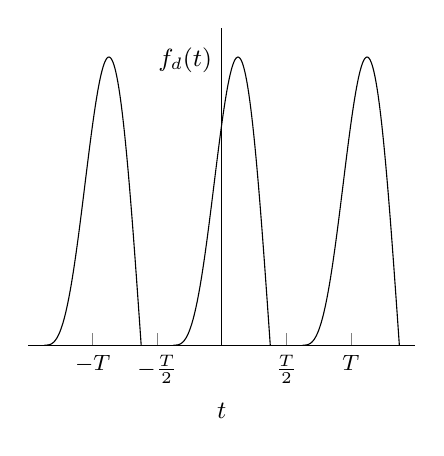
\begin{tikzpicture}
\begin{axis}[small,axis lines*=middle,xtick={-240,-120,0,120,240},xticklabels={$-T$,$-\frac{T}{2}$,$0$,$\frac{T}{2}$,$T$},ytick=\empty,ymin=0,xmin=-360,xmax=360,ylabel={$f_d(t)$},xlabel={$t$},ylabel style={rotate=-90,at={(axis description cs:0.5,0.9)}}]
\addplot[domain=-90:90,samples=100]{cos(x)+1/2*sin(2*x)};
\addplot[domain=240-90:240+90,samples=100]{cos(x-240)+1/2*sin(2*(x-240))};
\addplot[domain=-240-90:-240+90,samples=100]{cos(x+240)+1/2*sin(2*(x+240))};
\end{axis}
\end{tikzpicture}
\caption*{(ب) دوری تفاعل۔}
\end{subfigure}
\caption{دوری اور غیر دوری تفاعل۔}
\label{شکل_فوریئر_دوری_غیر_دوری}
\end{figure}

دوری تفاعل کے لکیری طیف میں لکیریں ہارمونی تعدد \عددی{n\omega_0} پر پائی جاتی ہے لہٰذا دو قریبی لکیروں کے مابین تعددی فاصلہ
\begin{align}
\Delta \omega=(n+1)\omega_0-n\omega_0 =\omega_0=\frac{2\pi}{T}
\end{align}
ہو گا۔شکل \حوالہ{شکل_فوریئر_بدل_الف}-الف میں ان حقائق کی وضاحت کی گئی ہے۔دوری فاصلہ \عددی{T} بڑھانے سے طیفی لکیروں کے مابین تعددی فاصلہ کم ہو گا۔شکل-ب اور پ میں ایسا دکھایا گیا ہے۔جیسا شکل-ت میں دکھایا گیا ہے، \عددی{T \to \infty} کرنے سے \عددی{\Delta \omega \to \dif \omega} ہو گا، طیف اپنی لکیری خاصیت کھو دے گا اور یہ ایک مسلسل طیف کی صورت اختیار کر لیگا۔ایسی صورت میں طیف انفرادی تعدد \عددی{n\omega_0} کی بجائے تمام تعدد \عددی{\omega} پر پایا جائے گا لہٰذا \عددی{n\omega_0} کو \عددی{\omega} فرض کیا جا سکتا ہے یعنی
\begin{align}\label{مساوات_فوریئر_لامتناہی_دوری_عرصہ_تعددی_فرق}
n \omega_0 = \omega
\end{align}
%
 \begin{figure}
\centering
\begin{subfigure}{0.5\textwidth}
\centering
\begin{tikzpicture}
\draw(0,0)--++(4,0)node[below]{$\omega$};
\draw(0,0)--++(0,2)node[left]{$D_n$};
\foreach \kx in {1,2,3,4,5}{\draw(\kx*0.72,0)--++(0,{1.75*cos(\kx*12.6)})node[circ]{};}
\draw(0.72,0)node[below]{$1\omega_0$};
\draw(0.72*2,0)node[below]{$2\omega_0$};
\draw(0.72*3,-0.1)--++(0,-0.3);
\draw(0.72*4,-0.1)--++(0,-0.3);
\draw[stealth-stealth](0.72*3,-0.2)--(0.72*4,-0.2)node[pos=0.5,below]{$\Delta \omega$};
\end{tikzpicture}
\caption*{طیفی لکیروں کے مابین فاصلہ \عددی{\omega_0} ہے۔}
\end{subfigure}%
\begin{subfigure}{0.5\textwidth}
\centering
\begin{tikzpicture}
\draw(0,0)--++(4,0)node[below]{$\omega$};
\draw(0,0)--++(0,2)node[left]{$D_n$};
\foreach \kx in {1,2,...,18}{\draw(\kx*0.2,0)--++(0,{1.75*cos(\kx*3.5)})node[circ]{};}
\end{tikzpicture}
\caption*{(ب) دوری عرصہ بڑھانے سے طیفی\\ لکیروں کے مابین فاصلہ کم ہوتا ہے۔}
\end{subfigure}
\begin{subfigure}{0.5\textwidth}
\centering
\begin{tikzpicture}
\draw(0,0)--++(4,0)node[below]{$\omega$};
\draw(0,0)--++(0,2)node[left]{$D_n$};
\foreach \kx in {1,2,...,36}{\draw(\kx*0.1,0)--++(0,{1.75*cos(\kx*1.75)})node[circ]{};}
\end{tikzpicture}
\caption*{(پ) دوری عرصہ بہت بڑھانے سے طیفی لکیروں\\ کے مابین فاصلہ نہایت کم ہو جاتا ہے۔}
\end{subfigure}%
\begin{subfigure}{0.5\textwidth}
\centering
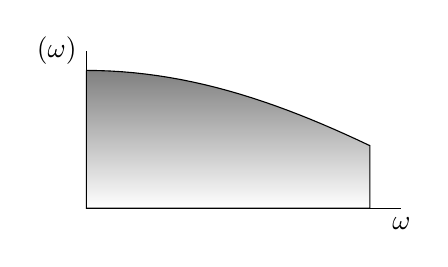
\begin{tikzpicture}
\draw(0,0)--++(4,0)node[below]{$\omega$};
\draw(0,0)--++(0,2)node[left]{$\Fourier(\omega)$};
\draw[shade,domain=0:63,variable=\t] plot ({\t*2/35},{1.75*cos(\t)}) --(3.6,0)--(0,0)--(0,1.75);
\end{tikzpicture}
\caption*{(ت) لامتناہی دوری عرصے کی صورت میں طیفی لکیریں آپس\\ میں مل جاتی ہیں اور ان میں فرق کرنا ممکن نہیں رہتا۔}
\end{subfigure}
\caption{لکیری طیف سے مسلسل طیف کا حصول۔}
\label{شکل_فوریئر_بدل_الف}
\end{figure}

چونکہ \عددی{T \to \infty} کرنے سے مساوات \حوالہ{مساوات_فوریئر_لکیری_طیف_عددی_سر} میں \عددی{\kx{c}_n \to 0} ہوں گے لہٰذا ہم \عددی{\kx{c}_n T} پر نظر رکھتے ہوئے آگے بڑھتے ہیں۔
\begin{align*}
\kx{c}_n T=\int_{-\frac{T}{2}}^{\frac{T}{2}} f_d(t) e^{-jn\omega_0 t}\dif t
\end{align*}
دوری عرصے کی حد لامتناہی کرتے ہوئے درج بالا مساوات کو درج ذیل لکھا جا سکتا ہے
\begin{align*}
\lim_{T \to \infty} (\kx{c}_n T)&= \lim_{T \to \infty}\int_{-\frac{T}{2}}^{\frac{T}{2}} f_d(t) e^{-jn\omega_0 t}\dif t\\
&=\int_{-\infty}^{\infty} f(t) e^{-j\omega t}\dif t
\end{align*}
جہاں مندرجہ بالا بحث کو مد نظر رکھتے ہوئے، دوسری قدم پر دوری تفاعل \عددی{f_d(t)} کی جگہ غیر دوری تفاعل\عددی{f(t)} پر کیا گیا ہے اور مساوات \حوالہ{مساوات_فوریئر_لامتناہی_دوری_عرصہ_تعددی_فرق} کا استعمال کیا گیا ہے۔ اس تکمل کو \اصطلاح{فوریئر بدل}\فرہنگ{فوریئر بدل}\فرہنگ{بدل!فوریئر}\حاشیہب{Fourier transform}\فرہنگ{Fourier transform} کہتے اور \عددی{\Fourier(\omega)} سے ظاہر کیا جاتا ہے۔
\begin{align}\label{مساوات_فوریئر_الف}
\bF(\omega)=\int_{-\infty}^{\infty} f(t) e^{-j\omega t}\dif t
\end{align}
اسی طرح دوری تفاعل کو درج ذیل لکھا جا سکتا ہے
\begin{align*}
f_d(t)&=\sum_{n=-\infty}^{\infty} \kx{c}_n e^{jn\omega_0 t}\\
&=\sum_{n=-\infty}^{\infty} (\kx{c}_n T) e^{jn\omega_0 t} \frac{1}{T}\\
&=\sum_{n=-\infty}^{\infty} (\kx{c}_n T) e^{jn\omega_0 t} \frac{\Delta \omega}{2\pi}
\end{align*}
جس کو \عددی{T \to \infty} کی صورت میں درج ذیل لکھا جا سکتا ہے
\begin{align}\label{مساوات_فوریئر_ب}
f(t)=\frac{1}{2\pi}\int_{-\infty}^{\infty} \bF(\omega)e^{j\omega t} \dif \omega
\end{align}
جہاں مساوات \حوالہ{مساوات_فوریئر_لامتناہی_دوری_عرصہ_تعددی_فرق} کا استعمال کیا گیا ہے۔

مساوات \حوالہ{مساوات_فوریئر_الف} اور مساوات \حوالہ{مساوات_فوریئر_ب} فوریئر جوڑی کہلاتے ہیں۔چونکہ \عددی{f(t)} کا \اصطلاح{فوریئر بدل}\فرہنگ{فوریئر!بدل}\حاشیہب{Fourier transform}\فرہنگ{Fourier!transform} \عددی{\Fourier(\omega)} ہے لہٰذا \عددی{\Fourier(\omega)} کا \اصطلاح{الٹ فوریئر بدل}\فرہنگ{فوریئر!الٹ بدل}\حاشیہب{inverser Fourier transform}\فرہنگ{Fourier!inverse transform} \عددی{f(t)} ہے۔فوریئر جوڑی کو اکٹھے لکھتے ہیں۔
\begin{gather}
\begin{aligned}\label{مساوات_فوریئر_پ}
\bF(\omega)=\Fourier[f(t)]&=\int_{-\infty}^{\infty} f(t) e^{-j\omega t}\dif t\\
f(t)=\Fourier^{-1}[\bF(\omega)]&=\frac{1}{2\pi}\int_{-\infty}^{\infty} \bF(\omega)e^{j\omega t} \dif \omega
\end{aligned}
\end{gather}
%==========

\حصہء{چند اہم فوریئر بدل جوڑیاں}
چند فوریئر بدل کی جوڑیاں حاصل کرتے ہیں۔
%=======================
\ابتدا{مثال}\شناخت{مثال_فوریئر_مستطیل_کا_بدل}
شکل \حوالہ{شکل_فوریئر_مستطیل_کا_بدل}-الف میں دیے مستطیل تفاعل \عددی{f(t)} کی فوریئر بدل \عددی{\bF(\omega)} حاصل کریں۔
\begin{figure}
\centering
\begin{subfigure}{0.5\textwidth}
\centering
\begin{tikzpicture}
\begin{axis}[small,axis lines*=middle,ytick=\empty,xtick={-0.5,0,0.5},xticklabels={$-\frac{\delta}{2}$,$0$,$\frac{\delta}{2}$},xlabel={$t$},xmin=-6,xmax=6,ymin=0,ymax=1.5,ylabel={$v(t)$},ylabel style={rotate=-90},ylabel style={at={(axis description cs:0.5,0.9)}},xlabel style={at={(axis description cs:1.05,0)}}]
\addplot[] plot coordinates {(-0.5,0) (-0.5,1) (0.5,1) (0.5,0)};
\addplot[]plot coordinates{(-1.5,1)}node[font=\small]{$V$};
\end{axis}
\end{tikzpicture}
\caption*{(الف)}
\end{subfigure}%
\begin{subfigure}{0.5\textwidth}
\centering
\begin{tikzpicture}
\begin{axis}[small,axis lines*=middle,ytick=\empty,xtick={-5,-0.5,0,0.5,5},xticklabels={$-T$,$-\frac{\delta}{2}$,$0$,$\frac{\delta}{2}$,$T$},xlabel={$t$},xmin=-6,xmax=6,ymin=0,ymax=1.5,ylabel={$v_d(t)$},ylabel style={rotate=-90},ylabel style={at={(axis description cs:0.5,0.9)}},xlabel style={at={(axis description cs:1.05,0)}}]
\addplot[] plot coordinates {(-0.5,0) (-0.5,1) (0.5,1) (0.5,0)};
\addplot[] plot coordinates {(5-0.5,0) (5-0.5,1) (5+0.5,1) (5+0.5,0)};
\addplot[] plot coordinates {(-5-0.5,0) (-5-0.5,1) (-5+0.5,1) (-5+0.5,0)};
\addplot[stealth-stealth] plot coordinates {(0,0.5) (5,0.5)}node[pos=0.5,above]{$T=5\delta$};
\addplot[]plot coordinates{(-1.5,1)}node[font=\small]{$V$};
\end{axis}
\end{tikzpicture}
\caption*{(ب)}
\end{subfigure}
\begin{subfigure}{0.5\textwidth}
\centering
\begin{tikzpicture}
\begin{axis}[axis lines*=middle,ytick={1},yticklabels={$V \delta$},xtick={-360,-180,0,180,360},xticklabels={$-\frac{4\pi}{\delta}$,$-\frac{2\pi}{\delta}$,$0$,$\frac{2\pi}{\delta}$,$\frac{4\pi}{\delta}$},xlabel={$\omega$},xlabel style={at={(axis description cs:1.05,0.2)}},ylabel={$\bF(\omega)$},ylabel style={rotate=-90},ylabel style={at={(axis description cs:0.5,1)}},ymax=1.3]
\addplot [domain = -600:600, samples = 100]{sin(x)/ (x*pi/180) };
\end{axis}
\end{tikzpicture}
\caption*{(پ)}
\end{subfigure}
\begin{subfigure}{0.5\textwidth}
\centering
\begin{tikzpicture}
\begin{axis}[axis lines*=middle,ytick={1},yticklabels={$\frac{V \delta}{T}$},xlabel={$\omega$},xlabel style={at={(axis description cs:1.05,0.2)}},ylabel={$\kx{c}_n$},ylabel style={rotate=-90},ylabel style={at={(axis description cs:0.5,1)}},ymax=1.3,xtick=\empty]
\addplot [domain = -600:600, samples = 100]{sin(x)/ (x*pi/180) }node[pos=0.55,pin=45:{غلاف}]{};
%
\addplot[] plot coordinates {(36,0) (36,{sin(36)/ (36*pi/180) })};
\addplot[] plot coordinates {(72,0) (72,{sin(72)/ (72*pi/180) })};
\addplot[] plot coordinates {(108,0) (108,{sin(108)/ (108*pi/180) })};
\addplot[] plot coordinates {(144,0) (144,{sin(144)/ (144*pi/180) })};
\addplot[] plot coordinates {(216,0) (216,{sin(216)/ (216*pi/180) })};
\addplot[] plot coordinates {(252,0) (252,{sin(252)/ (252*pi/180) })};
\addplot[] plot coordinates {(288,0) (288,{sin(288)/ (288*pi/180) })};
\addplot[] plot coordinates {(324,0) (324,{sin(324)/ (324*pi/180) })};
%

\addplot[] plot coordinates {(-36,0) (-36,{sin(-36)/ (-36*pi/180) })};
\addplot[] plot coordinates {(-72,0) (-72,{sin(-72)/ (-72*pi/180) })};
\addplot[] plot coordinates {(-108,0) (-108,{sin(-108)/ (-108*pi/180) })};
\addplot[] plot coordinates {(-144,0) (-144,{sin(-144)/ (-144*pi/180) })};
\addplot[] plot coordinates {(-216,0) (-216,{sin(-216)/ (-216*pi/180) })};
\addplot[] plot coordinates {(-252,0) (-252,{sin(-252)/ (-252*pi/180) })};
\addplot[] plot coordinates {(-288,0) (-288,{sin(-288)/ (-288*pi/180) })};
\addplot[] plot coordinates {(-324,0) (-324,{sin(-324)/ (-324*pi/180) })};
%
\addplot[]plot coordinates {(180,-0.1) (180,-0.2)};
\addplot[stealth-stealth]plot coordinates {(0,-0.15) (180,-0.15)}node[pos=0.5,below]{$\frac{2\pi}{\delta}$};
\addplot[-stealth]plot coordinates {(18,0.3) (72,0.3)};
\addplot[stealth-]plot coordinates {(108,0.3) (180,0.3) (200,0.35)}node[right]{$\frac{2\pi}{T}$};
\end{axis}
\end{tikzpicture}
\caption*{(ت)}
\end{subfigure}
\caption{مثال \حوالہ{مثال_فوریئر_مستطیل_کا_بدل} کا تفاعل۔}
\label{شکل_فوریئر_مستطیل_کا_بدل}
\end{figure}

حل:مساوات \حوالہ{مساوات_فوریئر_پ} استعمال کرتے ہوئے فوریئر بدل حاصل کرتے ہیں۔
\begin{align*}
\bF(\omega)&=\int_{-\frac{\delta}{2}}^{\frac{\delta}{2}} V e^{-j\omega t} \dif t\\
&=\left. \frac{V e^{-j\omega t}}{-j\omega}\right|_{-\frac{\delta}{2}}^{\frac{\delta}{2}}\\
&=V\frac{e^{-j\omega \frac{\delta}{2}}-e^{+j\omega \frac{\delta}{2}}}{j\omega}\\
&=V \delta \frac{\sin \frac{\omega \delta}{2}}{\frac{\omega \delta}{2}}
\end{align*}
یوں وقتی دائرہ کار کے تفاعل \عددی{f(t)}
\begin{align}
f(t)=
\begin{cases}
0 & -\infty < t \le -\frac{\delta}{2}\\
V & -\frac{\delta}{2} < t < \frac{\delta}{2}\\
0& \frac{\delta}{2} \le t < \infty
\end{cases}
\end{align}
کا فوریئر بدل \عددی{\bF(\omega)} درج ذیل ہے۔
\begin{align}
\bF(\omega)=\Fourier[f(t)]=V \delta \frac{\sin \frac{\omega \delta}{2}}{\frac{\omega \delta}{2}}
\end{align}
اس مثال پر مزید غور کرتے ہیں۔شکل \حوالہ{شکل_فوریئر_مستطیل_کا_بدل}-الف کے تفاعل کو شکل-ب میں \عددی{T} فاصلے کے دورانیے پر دہراتے ہوئے  دوری تفاعل \عددی{f_d(t)} حاصل کیا گیا ہے۔دوری تفاعل \عددی{f_d(t)} کے فوریئر تسلسل کے عددی سر درج ذیل ہیں۔
\begin{align}
\kx{c}_n=\frac{V \delta}{T} \frac{\sin\frac{n\omega_0 \delta}{2}}{\frac{n\omega_0 \delta}{2}}
\end{align}
شکل \حوالہ{شکل_فوریئر_مستطیل_کا_بدل}-ت میں لکیری طیف دکھائی گئی ہے۔آپ دیکھ سکتے ہیں کہ  لکیری طیف کے \اصطلاح{غلاف}\فرہنگ{غلاف}\حاشیہب{envelope}\فرہنگ{envelope} کی شکل اور مسلسل طیف کی شکل بالکل یکساں ہیں۔

اس مثال کے نتائج اور مساوات سے ظاہر ہے کہ \عددی{T \to \infty} کرنے سے دوری تفاعل تبدیل ہو کر غیر دوری تفاعل بن جاتا ہے۔ساتھ ہی ساتھ جیسے جیسے \عددی{T} بڑھتا ہے ویسے ویسے طیفی لکیر قریب ہوتے ہیں اور ان کا حیطہ کم  ہوتا ہے حتٰی کہ آخر کار لکیری طیف مسلسل طیف میں تبدیل ہو جاتا ہے۔چونکہ فوریئر تسلسل مخصوص تعدد پر اشارے کا حیطہ اور زاویائی ہٹاو دیتا ہے لہٰذا فوریئر بدل بھی اشارے کی تعددی معلومات دیتا ہے۔ 
\انتہا{مثال}
%=======================
\ابتدا{مثال}
اکائی ضرب تفاعل \عددی{\delta(t-a)} اور \عددی{\delta(t)} کا فوریئر بدل حاصل کریں۔

حل:اکائی ضرب تفاعل کا فوریئر بدل تکمل سے حاصل کرتے ہیں۔
\begin{gather}
\begin{aligned}
\bF(\omega)&=\int_0^{\infty} \delta(t-a)e^{-j\omega t} \dif t\\
&=e^{-j\omega a}
\end{aligned}
\end{gather}
تکمل کو حل میں اکائی ضرب تفاعل کی \اصطلاح{نمونہ بندی}\فرہنگ{نمونہ بندی!خاصیت}\فرہنگ{sampling!property} خاصیت استعمال کی گئی۔ درج بالا میں \عددی{a=0} پر کرنے سے اکائی ضرب تفاعل \عددی{\delta(t)} کا فوریئر بدل ملتا ہے۔
\begin{align}
\Fourier[\delta(t)]=1
\end{align}
آپ نے دیکھا کہ اکائی ضرب تفاعل \عددی{\delta(t)} کا فوریئر بدل ایک مستقل مقدار ہے جو تعدد کے ساتھ تبدیل نہیں ہوتا۔یہ اکائی ضرب تفاعل کی ایک اہم خصوصیت ہے۔
 
\انتہا{مثال}
%======================
\ابتدا{مثال}
تفاعل \عددی{e^{j\omega_0 t}} کا فوریئر بدل حاصل کریں۔

حل:یہاں اگر \عددی{\bF(\omega)=2\pi \delta(t-t_0)} لیا جائے تب \عددی{f(t)} درج ذیل ہو گا
\begin{gather}
\begin{aligned}
f(t)&=\frac{1}{2\pi}\int_{-\infty}^{\infty} 2\pi \delta(t-t_0)e^{j\omega t}\dif \omega\\
&=e^{j\omega_0 t}
\end{aligned}
\end{gather} 
جہاں \عددی{\delta(t-t_0)} کی نمونہ بندی کی خاصیت استعمال کی گئی۔یوں \عددی{f(t)=e^{j\omega_0 t}} اور \عددی{\bF(\omega)=2\pi\delta(t-t_0)} فوریئر بدل جوڑی ہیں۔ 
\انتہا{مثال}
%=======================
\ابتدا{مشق}
تفاعل \عددی{\cos \omega t} کا فوریئر بدل دریافت کریں۔

جواب:\عددی{\bF(\omega)=\pi \delta(\omega-\omega_0)+\pi\delta(\omega+\omega_0)}
\انتہا{مشق}
%======================
چند اہم فوریئر بدل جوڑیوں کو جدول \حوالہ{جدول_فوریئر_بدل_جوڑیاں} میں اکٹھے کیا گیا ہے۔
\begin{table}
\caption{فوریئر بدل جوڑیاں۔}
\label{جدول_فوریئر_بدل_جوڑیاں}
\centering
\begin{tabular}{l l}
$\Fourier(\omega)$ & $f(t)$ \Bstrut \\
\hline
$2\pi A \delta(\omega)$&$A$ \Tstrut \\[2ex]
$1$&$\delta(t)$\\[1ex]
$e^{-j\omega a}$&$\delta(t-t_0)$\\[1ex]
 $2\pi \delta(\omega-\omega_0)$ &$e^{j\omega_0 t}$ \\[1ex]
 $j\pi \delta(\omega+\omega_0)-j\pi\delta(\omega-\omega_0)$ &$\sin \omega_0 t$ \\[1ex]
 $\pi \delta(\omega-\omega_0)+\pi\delta(\omega+\omega_0)$ &$\cos \omega_0 t$ \\[1ex]
 $\frac{1}{a+j\omega}$&$e^{-at}u(t), \, a>0$  \\[1ex]
 $\frac{2a}{a^2+\omega^2}$&$e^{-a\abs{t}}u(t), \, a>0 $  \\[1ex]
 $\frac{\omega_0}{(j\omega+0)^2+\omega_0^2}$ &$e^{-at} \sin \omega_0 t\, u(t), \, a>0$ \\[1ex]
 $\frac{j\omega+a}{(j\omega+0)^2+\omega_0^2}$ &$e^{-at} \cos \omega_0 t\, u(t), \, a>0$ 
\end{tabular}
\end{table}

%=============
\حصہ{فوریئر بدل کے خواص}
فوریئر بدل کے چند مخصوص مسئلوں کو جدول \حوالہ{جدول_فوریئر_بدل_مسئلے} میں پیش کیا گیا ہے۔ان میں سے \اصطلاح{مسئلہ وقتی الجھاو}\فرہنگ{مسئلہ!وقتی الجھاو}\فرہنگ{وقتی الجھاو!مسئلہ}\حاشیہب{time convolution theorem}\فرہنگ{time convolution!theorem}\فرہنگ{theorem!time convolution} کو ثابت کرتے ہیں۔جدول میں دیے بقایا مسئلے بھی انتہائی آسانی سے ثابت کئے جا سکتے ہیں۔
 
تفاعل \عددی{f(t)} کا فوریئر بدل درج ذیل ہے۔
\begin{align}
\Fourier[f(t)]=\bF(\omega)=\int_{-\infty}^{\infty}f(t) e^{-j\omega t} \dif t
\end{align}
فرض کریں کہ 
\begin{align*}
\Fourier[f_1(t)]&=\bF_1(\omega)\\
\Fourier[f_2(t)]&=\bF_2(\omega)
\end{align*}
ہیں تب
\begin{align*}
\Fourier\left[\int_{-\infty}^{\infty}f_1(x)f_2(t-x)\dif x\right]&=\int_{t=-\infty}^{\infty}\int_{x=-\infty}^{\infty}f_1(x)f_2(t-x)\dif x  e^{-j\omega t}\dif t\\
&=\int_{x=-\infty}^{\infty}f_1(x)\int_{t=-\infty}^{\infty}f_2(t-x)  e^{-j\omega t}\dif t \dif x
\end{align*}
اب  اگر ہم \عددی{u=t-x} پر کریں  تب درج ذیل لکھا جا سکتا ہے۔
\begin{align*}
\Fourier\left[\int_{-\infty}^{\infty}f_1(x)f_2(t-x)\dif x\right]&=\int_{x=-\infty}^{\infty}f_1(x)\int_{t=-\infty}^{\infty}f_2(u)  e^{-j\omega (u+x)}\dif u \dif x\\
&=\int_{x=-\infty}^{\infty}f_1(x) e^{-j\omega x}\dif x \int_{t=-\infty}^{\infty}f_2(u)  e^{-j\omega u}\dif u \\
&=\bF_1(\omega) \bF_2(\omega)
\end{align*}
شکل \حوالہ{شکل_فوریئر_وقتی_الجھاو} کو دیکھتے ہوئے مسئلہ وقتی الجھاو کہتا ہے کہ اگر \عددی{\kB{V}_d(\omega)=\Fourier[v_d(t)]}،
 \عددی{\kB{H}(\omega)=\Fourier[h(t)]} اور \عددی{\kB{V}_0(\omega)=\Fourier[v_0(t)]} ہوں تب
\begin{align}\label{مساوات_فوریئر_حل_دور}
\kB{V}_0(\omega)=\bH(\omega) \kB{V}_d(\omega)
\end{align}
ہو گا۔
\begin{figure}
\centering
\begin{tikzpicture}
\draw(0,0) rectangle ++(\x,\y/2);
\draw(0,\y/4)--++(-\x/2,0)node[left]{$\kB{V}_d(\omega)$};
\draw[-latex](\x,\y/4)--++(\x/2,0)node[right]{$\kB{V}_0(\omega)=\bH(\omega) \kB{V}_d(\omega)$};
\draw(\x/2,\y/4)node{$\bH(\omega)$};
\end{tikzpicture}
\caption{وقتی الجھاو۔}
\label{شکل_فوریئر_وقتی_الجھاو}
\end{figure}
%================
\begin{table}
\caption{فوریئر بدل کے مسئلے۔}
\label{جدول_فوریئر_بدل_مسئلے}
\centering
\begin{tabular}{l l r}
$\Fourier(\omega)$ & $f(t)$ & مسئلہ \Bstrut \\ 
\hline
$A\bF(\omega) $& $Af(t)$ & خطیت\Tstrut \\ [2ex]
$\bF_1(\omega)\mp \bF_2(\omega) $& $f_1(t)\mp f_2(t)$&\\[2ex]
$\frac{1}{a}\bF\left(\frac{\omega}{a}\right), \, a>0 $& $f(at)$ & مسئلہ متناسب وقت\\[2ex]
$e^{-j\omega t_0} \bF(\omega)$ &$ f(t-t_0)$ & مسئلہ منتقلی وقت\\[2ex]
$\bF(\omega-\omega_0)$ & $e^{j\omega t_0} f(t)$ & ترمیم تعدد\\[2ex]
$(j\omega)^n \bF(\omega)$ &$\frac{\dif^{\,n} f(t)}{\dif t^n}$ & \\[2ex]
$(j)^n \frac{\dif^{\, n} \bF(\omega)}{\dif \omega^n}$&$t^n f(t)$&تفرق\\[2ex]
$\bF_1(\omega)\bF_2(\omega)$ & $\int_{-\infty}^{\infty} f_1(x) f_2(t-x) \dif x$ & \\[2ex]
$\frac{1}{2\pi} \int_{-\infty}^{\infty} \bF_1(x)\bF_2(\omega-x) \dif x$&$f_1(t) f_2(t)$&الجھاو  
\end{tabular}
\end{table}
%==================

\ابتدا{مشق}\شناخت{مشق_فوریئر_دور_کا_حل}
شکل \حوالہ{شکل_فوریئر_دور_کا_حل} میں داخلی دباو \عددی{v_d(t)=e^{-t}u(t)\,\si{\volt}}،  دور کا اکائی ضرب رد عمل \عددی{h(t)=e^{-2t}u(t)} جبکہ ابتدائی معلومات صفر ہیں۔خارجی دباو \عددی{v_0(t)} دریافت کریں۔
\begin{figure}
\centering
\begin{tikzpicture}
\draw(0,0) rectangle ++(\x,\y/2);
\draw(0,\y/4)--++(-\x/2,0)node[left]{$v_d(t)$};
\draw[-latex](\x,\y/4)--++(\x/2,0)node[right]{$v_0(t)$};
\draw(\x/2,\y/4)node{$h(t)$};
\end{tikzpicture}
\caption{مشق \حوالہ{مشق_فوریئر_دور_کا_حل} کا دور۔}
\label{شکل_فوریئر_دور_کا_حل}
\end{figure}


جواب:\عددی{v_0(t)=(e^{-t}-e^{-2t})u(t)\,\si{\volt}}
\انتہا{مشق}
%================
\ابتدا{مشق}\شناخت{مشق_فوریئر_دور_کا_حل_ب}
شکل \حوالہ{شکل_فوریئر_دور_کا_حل_ب} میں \عددی{v_d(t)=42\cos 3t \,\si{\volt}} ہے۔فوریئر بدل کے طریقے سے \عددی{v_0(t)} حاصل کریں۔
\begin{figure}
\centering
\begin{tikzpicture}[american voltages]
\draw(0,0) to [american voltage source,l={$v_d(t)$}]++(0,\y) to [resistor,l={$\SI{2}{\ohm}$}]++(\x,0) to [capacitor,l={$\SI{0.2}{\farad}$}]++(\x,0) to [resistor,l_={$\SI{1}{\ohm}$},v^<={$v_0(t)$}]++(0,-\y) to [short] (0,0);
\draw (\x,0) to [inductor,*-*,l={$\SI{0.4}{\henry}$}]++(0,\y);
\end{tikzpicture}
\caption{مشق \حوالہ{مشق_فوریئر_دور_کا_حل_ب} کا دور۔}
\label{شکل_فوریئر_دور_کا_حل_ب}
\end{figure}

جواب:\عددی{v_0(t)=12.57\cos(10t+86.2^{\circ})\,\si{\volt}}
\انتہا{مشق}
%=================

\حصہ{مسئلہ پارسیوال}
\اصطلاح{مسئلہ پارسیوال}\فرہنگ{مسئلہ!پارسیوال}\حاشیہب{Parseval's theorem}\فرہنگ{Parseval's theorem}\فرہنگ{theorem!Parseval} کی الجبرائی صورت درج ذیل ہے۔
\begin{align}
\int_{-\infty}^{\infty} f^2(t) \dif t=\frac{1}{2\pi}\int_{-\infty}^{\infty} \abs{\bF(\omega)}^2\dif \omega
\end{align}
اس تعلق کو حاصل کرتے ہیں۔
\begin{align*}
\int_{-\infty}^{\infty} f^2(t) \dif t&=\int_{-\infty}^{\infty} f(t) \frac{1}{2\pi} \int_{-\infty}^{\infty} \bF(\omega) e^{j\omega t} \dif \omega \dif t\\
&= \frac{1}{2\pi} \int_{-\infty}^{\infty}\bF(\omega)\int_{-\infty}^{\infty}  f(t) e^{-j(-\omega) t} \dif t \dif \omega \\
&= \frac{1}{2\pi} \int_{-\infty}^{\infty}\bF(\omega)\bF(-\omega) \dif \omega \\
&=\frac{1}{2\pi}  \int_{-\infty}^{\infty} \bF(\omega)\bF^*(\omega) \dif \omega \\
&=\frac{1}{2\pi}  \int_{-\infty}^{\infty} \abs{\bF(\omega)}^2\dif \omega 
\end{align*}
فرض کریں کہ \عددی{\SI{1}{\ohm}} کی مزاحمت میں رو \عددی{f(t)} ہے۔اس مزاحمت میں طاقت \عددی{f^2(t)} اور توانائی کا ضیاع \عددی{\int f^2(t) \dif t} ہو گا۔مسئلہ پارسیوال کہتا ہے کہ \عددی{\SI{1}{\ohm}} کی مزاحمتی ضیاع یا تقابل پذیر ضیاع کو وقتی دائرہ کار یا تعددی دائرہ کار میں حاصل کیا جا سکتا ہے۔ 

پٹی گزار چھلنی جو \عددی{\omega_1 \le \omega \le \omega_2} کے تعدد گزارتا ہو درج ذیل توانائی گزارے گی۔
\begin{align}
W=\int_{-\infty}^{\infty} f^2(t) \dif t&=\frac{1}{2\pi}  \int_{\omega_1}^{\omega_2} \abs{\bF(\omega)}^2\dif \omega 
\end{align}
یوں \عددی{\Delta \omega} کی باریک تعددی پٹی میں درج ذیل توانائی پائی جائے گی۔
\begin{align}
\Delta W=\frac{1}{2\pi} \abs{\bF(\omega)}^2 \Delta \omega
\end{align}
اگرچہ توانائی کو پارسیوال تکمل کے دونوں اطراف سے حاصل کیا جا سکتا ہے، تعددی دائرہ کار میں توانائی کسی مخصوص تعددی پٹی میں بھی حاصل کی جا سکتی ہے۔
%==============
\ابتدا{مثال}\شناخت{مثال_فوریئر_مزاحمت_امالہ}
شکل \حوالہ{شکل_فوریئر_مزاحمت_امالہ} میں \عددی{v_d(t)=10e^{-4t} u(t)\,\si{\volt}} کی صورت میں \عددی{v_0(t)} فوریئر طریقے سے حاصل کریں۔ اسی دور کو فوریئر طریقے سے \عددی{v_d(t)=15\cos 5t\,\si{\volt}} کے لئے بھی حل کریں۔ 
\begin{figure}
\centering
\begin{tikzpicture}[american voltages]
\draw(0,0) to [american voltage source,l={$v_d(t)$}]++(0,\y) to [resistor,l={$\SI{4}{\ohm}$}]++(\x,0) to [capacitor,l_={$\SI{0.5}{\farad}$},v^<={$v_0(t)$}]++(0,-\y) to [short] (0,0);
\end{tikzpicture}
\caption{مثال \حوالہ{مثال_فوریئر_مزاحمت_امالہ} اور مثال \حوالہ{مثال_فوریئر_مزاحمت_برق_گیر} کا دور۔}
\label{شکل_فوریئر_مزاحمت_امالہ}
\end{figure}

حل:داخلی دباو \عددی{v_d(t)} کا فوریئر بدل جدول \حوالہ{جدول_فوریئر_بدل_جوڑیاں} سے لکھتے ہیں۔
\begin{align*}
\bV_d(\omega)=\frac{10}{4+j\omega}
\end{align*}
دور کا \عددی{\bH(\omega)} درج ذیل ہے۔
\begin{align*}
\bH(\omega)=\frac{1}{1+j2\omega}
\end{align*}
مساوات \حوالہ{مساوات_فوریئر_حل_دور} کے تحت
\begin{align*}
\kB{V}_0(\omega)&=\bH(\omega) \kB{V}_d(\omega)\\
&=\frac{10}{(1+j2\omega)(4+j\omega)}\\
&=\frac{10}{7(j\omega+0.5)}-\frac{10}{7(j\omega+4)}
\end{align*}
ہو گا۔جدول \حوالہ{جدول_فوریئر_بدل_جوڑیاں} سے الٹ فوریئر بدل لیتے ہوئے درج ذیل حاصل ہوتا ہے۔
\begin{align*}
v_0(t)=\frac{10}{7} e^{-0.5t}u(t)-\frac{10}{7}e^{-4t}u(t) \,\si{\volt}
\end{align*}
آئیں اب \عددی{v_d(t)=15\cos 5t \,\si{\volt}} کا فوریئر بدل جدول سے لکھیں۔
\begin{align*}
\bV_d(\omega)&=15\pi\delta(\omega-5)+15\pi\delta(\omega+5)
\end{align*}
خارجی دباو لکھتے ہیں۔
\begin{align*}
\bV_0(\omega)&=\bH(\omega)\bV_d(\omega)\\
&=\frac{15\pi}{1+j2\omega}[\delta(\omega-5)+\delta(\omega+5)]
\end{align*}
فوریئر الٹ بدل لیتے ہیں
\begin{align*}
v_0(t)&=\frac{1}{2\pi}\int_{-\infty}^{\infty} 15\pi \frac{\delta(\omega-5)+\delta(\omega+5)}{1+j2\omega} e^{j\omega t} \dif \omega\\
&=7.5 \frac{e^{j5t}}{1+j10}+7.5\frac{e^{-j5t}}{1-j10}\\
&=\frac{7.5e^{5t}}{\sqrt{101}e^{j84.3^{\circ}}}+\frac{7.5e^{-5t}}{\sqrt{101}e^{-j84.3^{\circ}}}\\
&=1.493\cos(5t-84.3^{\circ})\,\si{\volt}
\end{align*}
جہاں تکمل کو نمونہ بندی کی خاصیت سے حاصل کیا گیا۔
\انتہا{مثال}
%================
\ابتدا{مثال}\شناخت{مثال_فوریئر_مزاحمت_برق_گیر}
شکل \حوالہ{شکل_فوریئر_مزاحمت_امالہ} میں  \عددی{v_d(t)=10e^{-4t} u(t)\,\si{\volt}} کی صورت میں داخلی اور خارجی تقابل پذیر توانائی دریافت کریں۔

حل:اکائی اوہم داخلی توانائی حاصل کرتے ہیں۔
\begin{align*}
W_d&=\int_0^{\infty} f^2(t) \dif t\\
&=\int_0^{\infty} 100 e^{-8t} \dif t\\
&=\left. \frac{100e^{-8t}}{-8}\right|_{0}^{\infty}\\
&=\SI{12.5}{\joule}
\end{align*}
خارجی توانائی کو مسئلہ پارسیوال سے حاصل کرتے ہیں۔گزشتہ مثال میں درج ذیل حاصل کیا گیا
 \begin{align*}
\kB{V}_0(\omega)&=\frac{10}{(j2\omega+1)(j\omega+4)}
\end{align*}
لہٰذا
\begin{align*}
\abs{\kB{V}_0}^2&=\frac{100}{(4\omega^2+1)(\omega^2+16)}\\
&=\frac{100}{63(\omega^2+0.25)}-\frac{100}{63(\omega^2+16)}
\end{align*}
ہو گا اور تقابل پذیر خارجی توانائی
\begin{align*}
W_d&=\frac{1}{2\pi}\int_{-\infty}^{\infty}\abs{\bV_0(\omega)}^2 \dif \omega\\
&=\frac{50}{63\pi}\left(\int_{-\infty}^{\infty}\frac{\dif \omega}{\omega^2+0.5^2}-\int_{-\infty}^{\infty}\frac{\dif \omega}{\omega^2+4^2} \right)\\
&=\frac{50}{63\pi}\left(\left. \frac{1}{0.5}\tan^{-1} \frac{\omega}{0.5} \right|_{-\infty}^{\infty}-\left. \frac{1}{4}\tan^{-1} \frac{\omega}{4} \right|_{-\infty}^{\infty}\right)\\
&=\frac{50}{63\pi}\left(\frac{\pi}{0.5}-\frac{\pi}{4}\right)\\
&=\frac{25}{18}\,\si{\joule}
\end{align*}
ہو گی۔
\انتہا{مثال}
%==============================
\ابتدا{مثال}
تفاعل \عددی{f(t)=e^{-at}u(t)} کی اکائی اوہم توانائی دریافت کریں۔وہ  انقطاعی تعدد \عددی{\omega_0} دریافت کریں جس سے کم تعدد کی پٹی میں \عددی{\SI{95}{\percent}} توانائی پائی جاتی ہو۔

حل:اکائی اوہم توانائی حاصل کرتے ہیں۔
\begin{align*}
W&=\int_{-\infty}^{\infty} f^2(t)\dif t\\
&=\int_{-\infty}^{\infty} e^{-2at}u(t) \dif t\\
&=&=\int_{0}^{\infty} e^{-2at} \dif t\\
&=\left. \frac{e^{-2at}}{-2a}  \right|_{0}^{\infty}\dif t\\
&=\frac{1}{2a}
\end{align*}
تفاعل کا فوریئر بدل درج ذیل ہے
\begin{align*}
\bF(\omega)=\frac{1}{j\omega+a}
\end{align*}
لہٰذا 
\begin{align*}
\frac{1}{2\pi}\int_{-\infty}^{\infty} \abs{\bF(\omega)}^2 \dif \omega=\frac{1}{2\pi}\int_{-\infty}^{\infty}\frac{\dif \omega}{\omega^2+a^2}  =\frac{1}{2a}
\end{align*}
ہو گا۔ درج بالا کو ثابت کیا جا سکتا ہے۔چونکہ \عددی{\bF(\omega)} جفت تفاعل ہے لہٰذا
\begin{align*}
\frac{1}{2\pi}\int_{-\infty}^{\infty}\frac{\dif \omega}{\omega^2+a^2}&=\frac{2}{2\pi}\int_{0}^{\infty}\frac{\dif \omega}{\omega^2+a^2}\\
&=\left. \frac{1}{\pi a} \tan^{-1}\frac{\omega}{a}\right|_{0}^{\infty}\\
&=\frac{1}{2a}
\end{align*}
ہم تعدد \عددی{\omega_0} جاننا چاہتے ہیں جس کے لئے درج ذیل لکھا جا سکتا ہے
\begin{align*}
\frac{0.95}{2a}&=\frac{1}{\pi}\int_0^{\omega_0} \frac{\dif \omega}{\omega^2+a^2}\\
&=\left. \frac{1}{\pi a} \tan^{-1}\frac{\omega}{a} \right|_0^{\omega_0}\\
&=\frac{1}{\pi a} \tan^{-1} \frac{\omega_0}{a}
\end{align*}
جس سے
\begin{align*}
\omega_0=\SI{12.706}{\radian}
\end{align*}
حاصل ہوتا ہے لہٰذا \عددی{\SI{95}{\percent}} توانائی \عددی{0 \le \omega \le \SI{12.706}{\radian}} کی پٹی میں پائی جاتی ہے۔ 
\انتہا{مثال}
%=============================
\ابتدا{مشق}
تفاعل \عددی{f(t)=e^{-4t}u(t)} کی اکائی اوہم توانائی وقتی دائرہ کار اور تعددی دائرہ کار میں حاصل کریں۔

جواب:\عددی{\SI{125}{\milli\joule}}
\انتہا{مشق}
%===============================

\ابتدا{مشق}
تفاعل \عددی{f(t)=e^{-4t}u(t)} کی اکائی اوہم توانائی \عددی{0 \le \omega \le \SI{1}{\radian}} کی پٹی میں حاصل کریں۔

جواب:\عددی{\SI{19.49}{\milli\joule}}
\انتہا{مشق}
%===============================
\ابتدا{مشق}\شناخت{مشق_فوریئر_امالی_دور_الف}
شکل \حوالہ{شکل_فوریئر_امالی_دور_الف} میں \عددی{v_0(t)} کی اکائی اوہم توانائی دریافت کریں۔
\begin{figure}
\centering
\begin{tikzpicture}[american voltages]
\draw(0,0) to [american voltage source,l={$6e^{-3t} u(t)$}]++(0,\y) to [resistor,l={$\SI{2}{\ohm}$}]++(\x,0) to [inductor,l_={$\SI{1}{\henry}$},v^<={$v_0(t)$}]++(0,-\y) to [short] (0,0);
\end{tikzpicture}
\caption{مشق \حوالہ{مشق_فوریئر_امالی_دور_الف} کا دور۔}
\label{شکل_فوریئر_امالی_دور_الف}
\end{figure}

جواب:\عددی{W=\SI{3.6}{\joule}}
\انتہا{مشق}
%===============================
\ابتدا{مثال}\شناخت{مثال_فوریئر_نشریات}
بے تار نشریات میں بلند تعدد \عددی{v_c(t)=A\cos \omega_c t} کے سائن نما سواری پر سمعی اشارہ \عددی{f_s} سوار کیا جاتا ہے۔ سمعی اشارے کی تعدد \عددی{\SI{20}{\hertz} \le f_s \le \SI{20000}{\hertz}} ہوتی ہے جبکہ \عددی{f_c} کی قیمت اس کی نسبت انتہائی زیادہ ہوتی ہے۔سمعی اشارے \عددی{v_s(t)} سے سواری اشارے کا حیطہ ترمیم کرتے ہوئے حیطہ سوار اشارہ حاصل کیا جاتا ہے جس کی الجبرائی صورت درج ذیل ہے۔
\begin{align}
v(t)=[A+v_s(t)]\cos(\omega_c t)
\end{align}
اینٹینا کے ذریعہ \عددی{v(t)} کو نشر کیا جاتا ہے۔اشارہ حاصل کرنے والا اینٹینا \عددی{v(t)} کا دھندلا نقش  حاصل کرتا ہے جس کا حیطہ نہایت کم لیکن صورت ہوبہو \عددی{v(t)} جیسے ہوتی ہے۔

آئیں سمعی اشارہ \عددی{v_s(t)}
\begin{align}
v_s(t)=\cos \omega_s t
\end{align}
اور  نشر اشارہ \عددی{v(t)}
\begin{align}
v(t)=[1+\cos \omega_s t] \cos \omega_c t
\end{align}
کے لکیری طیف حاصل کریں جہاں \عددی{f_s=\SI{1}{\kilo\hertz}}، \عددی{f_c=\SI{1260}{\kilo\hertz}} اور \عددی{A=1} ہیں۔پشاور شہر کے ریڈیو اسٹیشن کی نشریات \عددی{\SI{1260}{\kilo\hertz}} پر ہوتی ہے۔ 

سمعی اشارے کے فوریئر بدل
\begin{align}\label{مساوات_فوریئر_سمعی_اشارہ}
\bV_s(\omega)=\Fourier[\cos \omega_s t]=\pi \delta(\omega-\omega_s)+\pi\delta(\omega+\omega_s)
\end{align}
کو شکل \حوالہ{شکل_فوریئر_نشریات}-الف میں دکھایا گیا ہے۔نشر اشارے کو درج ذیل لکھتے
\begin{align*}
v(t)=[1+v_s(t)]\cos \omega_c t=\cos \omega_c t+v_s(t) \cos \omega_c t
\end{align*}
ہیں جس میں \عددی{\cos \omega_c t} کا فوریئر بدل
\begin{align}
\Fourier[\cos \omega_c t]=\pi \delta(\omega-\omega_c)+\pi\delta(\omega+\omega_c)
\end{align}
ہے جبکہ
\begin{align*}
v_s(t)\cos \omega_c t=v_s(t) \frac{e^{j\omega_c t}+e^{-j\omega_c t}}{2}
\end{align*}
لکھتے ہوئے  فوریئر بدل کے مسئلہ ترمیم کی مدد سے درج ذیل لکھا جا سکتا ہے۔
\begin{align*}
\Fourier[v_s(t)\cos \omega-c t]=\frac{1}{2}\left[\bV_s(\omega-\omega_c)+\bV_s(\omega+\omega_c)\right]
\end{align*}
مساوات \حوالہ{مساوات_فوریئر_سمعی_اشارہ} میں دیے سمعی اشارے کا بدل استعمال کرتے ہوئے یوں درج ذیل لکھا جا سکتا ہے۔
\begin{multline*}
\Fourier[v_s(t)\cos \omega_c t]=\frac{\pi}{2}\left[\delta(\omega-\omega_s-\omega_c)+\delta(\omega+\omega_s-\omega_c)\right.\\
\left.+\delta(\omega-\omega_s+\omega_c)+\delta(\omega+\omega_s+\omega_c)\right]
\end{multline*}
ان تمام کو استعمال کرتے ہوئے نشر اشارے کا بدل لکھتے ہیں جسے شکل \حوالہ{شکل_فوریئر_نشریات}-ب میں دکھایا گیا ہے۔
\begin{multline}
\bV(\omega)=\frac{\pi}{2}\left[2\delta(\omega-\omega_c)+2\delta(\omega+\omega_c)+\delta(\omega-\omega_s-\omega_c)\right.\\
\left.+\delta(\omega+\omega_s-\omega_c)+\delta(\omega-\omega_s+\omega_c)+\delta(\omega+\omega_s+\omega_c)\right]
\end{multline}
%
\begin{figure}
\centering
\begin{subfigure}{1\textwidth}
\centering
\begin{tikzpicture}
\draw(-2,0)--(2.5,0)node[right]{$f \,(\si{\hertz})$};
\draw(0,0)--++(0,2.5)node[left]{$\bV_s(\omega)$};
\draw[-latex](-1.5,0)node[below]{$-1000$}--++(0,1.5);
\draw[-latex](1.5,0)node[below]{$1000$}--++(0,1.5);
\draw(0,1.5)--++(-0.1,0)node[left]{$\pi$};
\end{tikzpicture}
\caption*{(الف) سمعی اشارے کا لکیری طیف۔}
\end{subfigure}
\begin{subfigure}{1\textwidth}
\centering
\begin{tikzpicture}
\draw(-5,0)--(5.5,0)node[right]{$f \,(\si{\kilo\hertz})$};
\draw(0,0)--++(0,2.5)node[left]{$\bV(\omega)$};
\draw[-latex](-3,0)node[below]{$-1260$}--++(0,1.5);
\draw[-latex](-4.5,0)node[below]{$-1261$}--++(0,0.75);
\draw[-latex](-1.5,0)node[below]{$-1259$}--++(0,0.75);
\draw[-latex](3,0)node[below]{$1260$}--++(0,1.5);
\draw[-latex](4.5,0)node[below]{$1261$}--++(0,0.75);
\draw[-latex](1.5,0)node[below]{$1259$}--++(0,0.75);
\draw(0,1.5)--++(-0.1,0)node[left]{$\pi$};
\draw(0,0.75)--++(-0.1,0)node[left]{$\frac{\pi}{2}$};
\end{tikzpicture}
\caption*{(ب) نشر اشارے کا لکیری طیف۔}
\end{subfigure}%
\caption{مثال \حوالہ{مثال_فوریئر_نشریات} کے لکیری طیف۔}
\label{شکل_فوریئر_نشریات}
\end{figure}
\انتہا{مثال}
%=================================
\ابتدا{مثال}\شناخت{مشق_فوریئر_انورٹر}
انجنیئرنگ کی ڈگری لینے کے بعد میری پہلی ذمہ داری سائن نما \اصطلاح{انورٹر}\فرہنگ{انورٹر}\حاشیہب{inverter}\فرہنگ{inverter} کی تخلیق\حاشیہد{میں نے کام کا آغاز اسلام آباد کے نجی ادارے \تحریر{rwr} (موجودہ نام) سے کیا جہاں میں نے سائن نما انورٹر پر ہی انجنیئرنگ تخلیق سیکھی۔} تھی۔انورٹر یک سمتی دباو کو بدلتے دباو میں تبدیل کرتا ہے۔غیر سائن نما انورٹر مستطیلی دباو پیدا کرتا ہے جس کو شکل \حوالہ{شکل_فوریئر_انورٹر} میں دکھایا گیا ہے۔آئیں اس پر غور کریں۔
\begin{figure}
\centering
\begin{tikzpicture}
\begin{axis}[xlabel={$t$},ylabel={$v(t)$},ylabel style={rotate=-90},ytick={-1,1},yticklabels={$-V_0$,$V_0$},xtick={-1.5,-0.75,0,0.75,1.5},xticklabels={$-\frac{T}{2}$,$-\frac{T}{4}$,$0$,$\frac{T}{4}$,$\frac{T}{2}$}]
\addplot[] plot coordinates{(-2.5,0)(-2,0)(-2,-1)(-1,-1)(-1,0)(-0.5,0)(-0.5,1) (0.5,1)(0.5,0)(1,0)(1,-1)(2,-1)(2,0) (2.5,0)(2.5,1)(3.5,1)(3.5,0)(4,0)};
\addplot[stealth-stealth] plot coordinates {(-0.5,0.5) (0.5,0.5)}node[pos=0.5,above]{$2\delta$};
\addplot[stealth-stealth] plot coordinates {(1,-0.5) (2,-0.5)}node[pos=0.5,above]{$2\delta$};
\end{axis}
\end{tikzpicture}
\caption{مشق \حوالہ{مشق_فوریئر_انورٹر} کے انورٹر کا مستطیلی دباو۔}
\label{شکل_فوریئر_انورٹر}
\end{figure}    

شکل میں دکھائے گئے دباو کی اوسط قیمت صفر ہے لہٰذا \عددی{a_0=0} ہو گا۔ساتھ ہی چونکہ دباو جفت ہے لہٰذا \عددی{b_n=0} ہوں گے۔آئیں \عددی{a_n} دریافت کریں۔
\begin{align*}
a_n&=\frac{4}{T}\int_0^{\frac{T}{2}} v(t)\cos (n\omega_0 t)\dif t\\
&=\frac{4}{T}\left[\int_0^{\delta} V_0\cos(n\omega_0 t) \dif t-\int_{\frac{T}{2}-\delta}^{\frac{T}{2}}V_0 \cos(n\omega_0 t)\dif t\right]\\
&=\frac{4V_0}{T}\left. \frac{\sin(n\omega_0 t)}{n\omega_0}\right|_{0}^{\delta}-\frac{4V_0}{T}\left. \frac{\sin(n\omega_0 t)}{n\omega_0}\right|_{\frac{T}{2}-\delta}^{\frac{T}{2}}\\
&=\frac{4V_0}{n\omega_0 T}\sin(n\omega_0 \delta)-\frac{4V_0}{n\omega_0 T}\sin\left(n\omega_0 \frac{T}{2}\right)+\frac{4V_0}{n\omega_0 T}\sin[n\omega_0 (\frac{T}{2}-\delta)]
\end{align*}
اس میں \عددی{\omega_0=\tfrac{2\pi}{T}} پر کرتے ہیں۔
\begin{align*}
a_n&=\frac{4V_0}{n\frac{2\pi}{T} T}\sin(n\frac{2\pi}{T}\delta)-\frac{4V_0}{n\frac{2\pi}{T} T}\sin\left(n\frac{2\pi}{T} \frac{T}{2}\right)+\frac{4V_0}{n\frac{2\pi}{T} T}\sin[n\frac{2\pi}{T} (\frac{T}{2}-\delta)]\\
&=\frac{2V_0}{n\pi}\sin(n\frac{2\pi}{T}\delta)-\frac{2V_0}{n\pi}\sin n\pi+\frac{2V_0}{n\pi}\sin[n\frac{2\pi}{T} (\frac{T}{2}-\delta)]\\
&=\frac{2V_0}{n\pi}\sin\left(\frac{2n\pi\delta}{T}\right)+\frac{2V_0}{n\pi}\sin\left(n\pi-\frac{2n\pi\delta}{T}\right)
\end{align*}
یہاں دائیں ہاتھ پر \عددی{\sin(\alpha-\beta)=\sin \alpha\cos \beta-\cos\alpha\sin\beta} استعمال کرتے ہیں۔
\begin{align*}
a_n&=\frac{2V_0}{n\pi}\sin\left(\frac{2n\pi\delta}{T}\right)+\frac{2V_0}{n\pi}\left[\sin n\pi \cos(\frac{2n\pi\delta}{T})-\cos n\pi \sin(\frac{2n\pi\delta}{T})\right]\\
&=\frac{2V_0}{n\pi}\sin\left(\frac{2n\pi\delta}{T}\right)-\frac{2V_0}{n\pi}\cos n\pi \sin(\frac{2n\pi\delta}{T})\\
&=\frac{2V_0}{n\pi}\sin\left(\frac{2n\pi\delta}{T}\right)(1-\cos n\pi)
\end{align*}
اس مساوات میں \عددی{n=1,2,3,\cdots} پر کرتے ہوئے چند عددی سر لکھتے ہیں۔
\begin{align*}
a_1&=\frac{4V_0}{\pi}\sin\frac{2\pi\delta}{T}\\
a_2&=0\\
a_3&=\frac{4V_0}{3\pi}\sin\frac{6\pi\delta}{T}\\
a_4&=0\\
a_5&=\frac{4V_0}{5\pi}\sin\frac{10\pi\delta}{T}
\end{align*}
ہم درج بالا عددی سر کی معلومات استعمال کرتے ہوئے \عددی{\delta} یوں رکھ سکتے ہیں کہ مخصوص عددی سر صفر کے برابر ہو جائے مثلاً \عددی{a_3} کی قیمت صفر کرنے کی خاطر \عددی{\tfrac{6\pi\delta}{T}=\pi} کرنا ہو گا یعنی \عددی{\delta=\tfrac{T}{3}} رکھا جائے گا۔
\انتہا{مثال}
%==================================
\ابتدا{مثال}\شناخت{مثال_فوریئر_دندانہ_چھلنی_متعدد}
شکل \حوالہ{شکل_فوریئر_دندانہ_چھلنی_متعدد}-الف میں \عددی{RLC} دندانہ چھلنی دکھائی گئی ہے۔سلسلہ وار \عددی{LC} کی قدرتی تعدد \عددی{\omega_0=\tfrac{1}{\sqrt{LC}}} پر ان کی سلسلہ وار رکاوٹ صفر ہو جاتی ہے لہٰذا \عددی{\omega_0} تعدد کا اشارہ خارجی جانب نہیں پایا جاتا۔اب تصور کریں کہ \عددی{\SI{500}{\hertz}} پر چلنے والے نظام کے قریب واپڈا کے \عددی{\SI{50}{\hertz}} دباو پر چلنے والی مشین \عددی{\SI{50}{\hertz}} اور اس کے دیگر ہارمونی تعدد کا برقی شور پیدا کرتی ہے جو \عددی{\SI{1}{\kilo\hertz}} کی نظام میں مداخلت پیدا کرتی ہے۔ان میں پہلا، دوسرا اور تیسرا ہارمونی شور زیادہ مسئلہ پیدا کرتے ہیں جن سے چھٹکارا ضروری ہے۔ 
\begin{figure}
\centering
\begin{subfigure}{1\textwidth}
\centering
\begin{tikzpicture}[american voltages]
\draw(0,0) to [american voltage source,l={$v_d(t)$}]++(0,2*\y) to [resistor,l={$R$}]++(\x,0) to [inductor,l_={$L$}]++(0,-\y) to [capacitor,l_={$C$}]++(0,-\y) to [short] (0,0);
\draw(\x,2*\y) to [short,*-o]++(\x,0);
\draw(\x,0) to [short,*-o]++(\x,0);
\draw(2*\x+0.25,\y) node{$\begin{aligned}&+ \\ \\ &v_0(t) \\ \\ &-  \end{aligned}$};
\end{tikzpicture}
\caption*{(الف)}
\end{subfigure}
\begin{subfigure}{1\textwidth}
\centering
\begin{tikzpicture}[american voltages]
\draw(0,0) to [american voltage source,l={$v_d(t)$}]++(0,2*\y) to [resistor,l={$R$}]++(\x,0) to [inductor,l_={$L_1$}]++(0,-\y) to [capacitor,l_={$C_1$}]++(0,-\y) to [short] (0,0);
\draw(\x,2*\y) to [short,*-]++(\x,0) to [inductor,l_={$L_2$}]++(0,-\y) to [capacitor,l_={$C_2$}]++(0,-\y) to [short,-*]++(-\x,0);
\draw(2*\x,2*\y) to [short,*-]++(\x,0) to [inductor,l_={$L_3$}]++(0,-\y) to [capacitor,l_={$C_3$}]++(0,-\y) to [short,-*]++(-\x,0);
\draw(3*\x,2*\y) to [short,*-o]++(\x,0);
\draw(3*\x,0) to [short,*-o]++(\x,0);
\draw(4*\x+0.25,\y) node{$\begin{aligned}&+ \\ \\ &v_0(t) \\ \\ &-  \end{aligned}$};
\end{tikzpicture}
\caption*{(ب)}
\end{subfigure}
\caption{مثال \حوالہ{مثال_فوریئر_دندانہ_چھلنی_متعدد} کی دندانہ چھلنی۔}
\label{شکل_فوریئر_دندانہ_چھلنی_متعدد}
\end{figure}

شکل \حوالہ{شکل_فوریئر_دندانہ_چھلنی_متعدد}-ب میں تین عدد \عددی{LC} جوڑیاں استعمال کی گئی ہیں جن میں \عددی{2\pi f_1=\tfrac{1}{\sqrt{L_1 C_1}}} رکھتے ہوئے \عددی{f_1=\SI{50}{\hertz}} کو رد کیا جاتا ہے۔اسی طرح \عددی{f_2=\SI{100}{\hertz}} کی دوسری ہارمونی اور \عددی{f_3=\SI{150}{\hertz}} کی تیسری ہارمونی کو  
\عددی{2\pi f_2=\tfrac{1}{\sqrt{L_2 C_2}}} اور \عددی{2\pi f_3=\tfrac{1}{\sqrt{L_3 C_3}}} چنتے ہوئے رد کیا جاتا ہے۔ 
\انتہا{مثال}

%=========================
\حصہء{سوالات}

%========================
\ابتدا{سوال}\شناخت{سوال_فوریئر_چکور_الف}
شکل \حوالہ{شکل_سوال_فوریئر_چکور_الف}-الف کے  عددی سر حاصل کرتے ہوئے اس کی تکونیاتی فوریئر تسلسل لکھیں۔
\begin{figure}
\centering
\begin{subfigure}{0.5\textwidth}
\centering
\begin{tikzpicture}
\begin{axis}[small,xtick={0,0.2,1,1.2},xticklabels={$0$,$0.2$,$1$,$1.2$},ytick={0,1},yticklabels={$0$,$1$},xlabel={$t$},ylabel={$v(t)$},ylabel style={rotate=-90},ylabel style={at={(axis description cs:0,1.05)}}]
\addplot[] plot coordinates {(-0.1,0) (0,0) (0,1) (0.2,1) (0.2,0) (1,0) (1,1) (1.2,1) (1.2,0) (1.5,0)};
\end{axis}
\end{tikzpicture}
\caption*{(الف)}
\end{subfigure}%
\begin{subfigure}{0.5\textwidth}
\centering
\begin{tikzpicture}
\begin{axis}[small,xtick={0,3,6,9,12},xticklabels={$0$,$3$,$6$,$9$,$12$},ytick={-1,0,1},yticklabels={$-1$,$0$,$1$},xlabel={$t$},ylabel={$i(t)$},ylabel style={rotate=-90},ylabel style={at={(axis description cs:0,1.05)}}]
\addplot[] plot coordinates {(-0.5,-1) (0,-1)(0,1)(3,1)(3,-1)(6,-1) (6,1) (9,1) (9,-1) (12,-1) (12,1) (12.4,1)};
\end{axis}
\end{tikzpicture}
\caption*{(ب)}
\end{subfigure}%
\caption{سوال \حوالہ{سوال_فوریئر_چکور_الف} کی موج۔}
\label{شکل_سوال_فوریئر_چکور_الف}
\end{figure}

جوابات:\عددی{a_0=0.2}، \عددی{a_n=\tfrac{1}{n\pi}\sin \tfrac{2\pi n}{5}}، \عددی{b_n=\tfrac{1}{n\pi}(1-\cos \tfrac{2\pi n}{5})}، \\
\begin{multline*}
v(t)=0.2+0.3027\cos (2\pi t) +0.2199\sin (2\pi t)+0.0935\cos(4\pi t)\\
+0.2879\sin(4\pi t)-0.0623\cos(6\pi t)+0.1919\sin(6\pi t)+\cdots
\end{multline*}
\انتہا{سوال}
%=========================
\ابتدا{سوال}\شناخت{سوال_فوریئر_چکور_ب}
شکل \حوالہ{شکل_سوال_فوریئر_چکور_الف}-ب کے تکونی فوریئر تسلسل کے عددی سر حاصل کریں۔تسلسل کے شروع کے چند ارکان لکھیں۔

جوابات:\عددی{a_0=0}، \عددی{a_n=0}، \عددی{b_n=\tfrac{2}{n\pi}(1-(-1)^n)}،
\begin{align*}
i(t)=\tfrac{4}{\pi}[\sin(\tfrac{\pi}{2}t)+\tfrac{1}{3}\sin(\tfrac{3\pi}{2}t)+\tfrac{1}{5}\sin(\tfrac{5\pi}{2}t)+\cdots]
\end{align*}
\انتہا{سوال}
%==========================
\ابتدا{سوال}\شناخت{سوال_فوریئر_چکور_پ}
شکل \حوالہ{شکل_سوال_فوریئر_چکور_پ}-الف کے  عددی سر حاصل کرتے ہوئے اس کی تکونیاتی فوریئر تسلسل لکھیں۔
\begin{figure}
\centering
\begin{subfigure}{0.5\textwidth}
\centering
\begin{tikzpicture}
\begin{axis}[small,xtick={0,1,2,3,4,5},xticklabels={$0$,$1$,$2$,$3$,$4$,$5$},ytick={0,1,2},yticklabels={$0$,$1$,$2$},xlabel={$t$},ylabel={$v(t)$},ylabel style={rotate=-90},ylabel style={at={(axis description cs:0,1.05)}}]
\addplot[] plot coordinates {(-0.5,0)(0,0)(0,2)(1,2)(1,1)(2,1) (2,0) (3,0)(3,2)(4,2)(4,1)(5,1) (5,0) (5.5,0)};
\end{axis}
\end{tikzpicture}
\caption*{(الف)}
\end{subfigure}%
\begin{subfigure}{0.5\textwidth}
\centering
\begin{tikzpicture}
\begin{axis}[small,xtick={0,1,2,3,4,5,6,7},xticklabels={$0$,$1$,$2$,$3$,$4$,$5$,$6$,$7$},ytick={0,1,2},yticklabels={$0$,$1$,$2$},xlabel={$t$},ylabel={$i(t)$},ylabel style={rotate=-90},ylabel style={at={(axis description cs:0,1.05)}}]
\addplot[] plot coordinates {(-0.5,0)(0,0)(0,1)(1,1)(1,2)(2,2) (2,1) (3,1)(3,0)(4,0)(4,1)(5,1) (5,2) (6,2) (6,1) (7,1) (7,0) (7.5,0)};
\end{axis}
\end{tikzpicture}
\caption*{(ب)}
\end{subfigure}%
\caption{سوال \حوالہ{سوال_فوریئر_چکور_پ} کی موج۔}
\label{شکل_سوال_فوریئر_چکور_پ}
\end{figure}

جوابات:
\begin{align*}
a_0&=1\\
a_n&=0\\
b_n&=\tfrac{3}{\pi}, \tfrac{3}{2\pi}, 0, \tfrac{3}{4\pi}, \tfrac{3}{5\pi}, 0, \tfrac{3}{7\pi}, \cdots\\
i(t)&=1+\tfrac{3}{\pi}(\sin \tfrac{2\pi t}{3}+\tfrac{1}{2}\sin \tfrac{4\pi t}{3}+\tfrac{1}{4}\sin \tfrac{8\pi t}{3}+\cdots)
\end{align*}
\انتہا{سوال}
%=========================
\ابتدا{سوال}\شناخت{سوال_فوریئر_چکور_ت}
شکل \حوالہ{شکل_سوال_فوریئر_چکور_پ}-ب کے تکونی فوریئر تسلسل کے عددی سر حاصل کریں۔تسلسل کے شروع کے چند ارکان لکھیں۔

جوابات:
\begin{align*}
a_0&=1\\
a_n&=-\tfrac{2}{\pi},0,\tfrac{2}{3\pi},0,-\tfrac{2}{5\pi},0,\tfrac{2}{7\pi},\cdots\\
b_n&=\tfrac{2}{\pi},0,\tfrac{2}{3\pi},0,\tfrac{2}{5\pi},0,\tfrac{2}{7\pi},\cdots\\
i(t)&=1-\tfrac{2}{\pi}(\cos \tfrac{\pi t}{2}-\sin \tfrac{\pi t}{2}-\tfrac{1}{3}\cos \tfrac{3\pi t}{2}-\tfrac{1}{3}\sin \tfrac{\pi t}{2}+\cdots  )
\end{align*}
\انتہا{سوال}
%==========================
\ابتدا{سوال}\شناخت{سوال_فوریئر_چکور_ٹ}
شکل \حوالہ{شکل_سوال_فوریئر_چکور_ٹ}-الف کے  عددی سر حاصل کرتے ہوئے اس کی تکونیاتی فوریئر تسلسل لکھیں۔
\begin{figure}
\centering
\begin{subfigure}{0.5\textwidth}
\centering
\begin{tikzpicture}
\begin{axis}[small,xtick={0,3,6,9},xticklabels={$0$,$3$,$6$,$9$},ytick={0,1},yticklabels={$0$,$1$},xlabel={$t$},ylabel={$v(t)$},ylabel style={rotate=-90},ylabel style={at={(axis description cs:0,1.05)}}]
\addplot[] plot coordinates {(0,0)(3,1)(3,0)(6,1)(6,0)(9,1)(9,0)};
\end{axis}
\end{tikzpicture}
\caption*{(الف)}
\end{subfigure}%
\begin{subfigure}{0.5\textwidth}
\centering
\begin{tikzpicture}
\begin{axis}[small,xtick={0,2,3,4,6,7,8},xticklabels={$0$,$2$,$3$,$4$,$6$,$7$,$8$},ytick={0,2},yticklabels={$0$,$2$},xlabel={$t$},ylabel={$i(t)$},ylabel style={rotate=-90},ylabel style={at={(axis description cs:0,1.05)}}]
\addplot[] plot coordinates {(-0.5,0)(0,0)(2,2)(3,2)(3,0)(4,0)(6,2)(7,2)(7,0)(7.5,0)};
\end{axis}
\end{tikzpicture}
\caption*{(ب)}
\end{subfigure}%
\caption{سوال \حوالہ{سوال_فوریئر_چکور_ٹ} کی موج۔}
\label{شکل_سوال_فوریئر_چکور_ٹ}
\end{figure}

جوابات:
\begin{align*}
a_0&=\tfrac{9}{4}\\
a_n&=0\\
b_n&=-\tfrac{9}{2n\pi}\\
v(t)&=\tfrac{9}{4}-\tfrac{9}{2\pi}\sum_{n=1}^{\infty} \tfrac{1}{n}\sin \tfrac{2n\pi t}{3}
\end{align*}
\انتہا{سوال}
%=========================
\ابتدا{سوال}\شناخت{سوال_فوریئر_چکور_ث}
شکل \حوالہ{شکل_سوال_فوریئر_چکور_ٹ}-ب کے تکونی فوریئر تسلسل کے عددی سر حاصل کریں۔

جوابات:
\begin{align*}
a_0&=1\\
a_n&=-\tfrac{2}{\pi}(1+\tfrac{2}{\pi}), \tfrac{2}{3\pi}(1-\tfrac{2}{3\pi}), -\tfrac{2}{5\pi}(1+\tfrac{2}{5\pi}), \tfrac{2}{7\pi}(1-\tfrac{2}{7\pi}),-\cdots\\
b_n&=0,\tfrac{1}{\pi},0, -\tfrac{1}{2\pi},0,\tfrac{1}{3\pi},0,-\cdots
\end{align*}
\انتہا{سوال}
%==========================
\ابتدا{سوال}\شناخت{سوال_فوریئر_چکور_ج}
شکل \حوالہ{شکل_سوال_فوریئر_چکور_ج}-الف کے  عددی سر حاصل کریں۔
\begin{figure}
\centering
\begin{subfigure}{0.5\textwidth}
\centering
\begin{tikzpicture}
\begin{axis}[small,xtick={-2,-1,0,1,2,4,5,7,8},xticklabels={$-2$,$-1$,$0$,$1$,$2$,$4$,$5$,$7$,$8$},ytick={0,1,4},yticklabels={$0$,$1$,$4$},xlabel={$t$},ylabel={$v(t)$},ylabel style={rotate=-90},ylabel style={at={(axis description cs:0,1.05)}}]
\addplot[] plot coordinates {(-2.5,0)(-2,0)(-2,1)(-1,1)(-1,4)(1,4)(1,1)(2,1)(2,0) (4,0)(4,1)(5,1)(5,4)(7,4)(7,1)(8,1)(8,0) (8.5,0)};
\end{axis}
\end{tikzpicture}
\caption*{(الف)}
\end{subfigure}%
\begin{subfigure}{0.5\textwidth}
\centering
\begin{tikzpicture}
\begin{axis}[small,xtick={-2,0,2,4,6},xticklabels={$-2$,$0$,$2$,$4$,$6$},ytick={0,1},yticklabels={$0$,$1$},xlabel={$t$},ylabel={$i(t)$},ylabel style={rotate=-90},ylabel style={at={(axis description cs:0,1.05)}}]
\addplot[] plot coordinates {(-2,0)(0,1)(2,0)(4,1) (6,0)};
\end{axis}
\end{tikzpicture}
\caption*{(ب)}
\end{subfigure}%
\caption{سوال \حوالہ{سوال_فوریئر_چکور_ج} کی موج۔}
\label{شکل_سوال_فوریئر_چکور_ج}
\end{figure}

جوابات:
\begin{align*}
a_0&=\tfrac{5}{3}\\
a_n&=\tfrac{2}{n\pi} (\sin \tfrac{2n\pi}{3}+3\sin\tfrac{n\pi}{3})\\
b_n&=0
\end{align*}
\انتہا{سوال}
%=========================
\ابتدا{سوال}\شناخت{سوال_فوریئر_چکور_چ}
شکل \حوالہ{شکل_سوال_فوریئر_چکور_ج}-ب کے تکونی فوریئر تسلسل کے عددی سر حاصل کریں۔

جوابات:
\begin{align*}
a_0&=\tfrac{1}{3}\\
a_n&=\tfrac{3}{n^2\pi^2}(1-\cos \tfrac{2n\pi}{3})\\
b_n&=0
\end{align*}
\انتہا{سوال}
%==========================


%============================
\ابتدا{سوال}\شناخت{سوال_فوریئر_سمت_کار_الف}
نصف لہر \اصطلاح{سمت کار}\فرہنگ{سمت کار!نصف لہر}\حاشیہب{half wave rectifier}\فرہنگ{rectifier!half wave} کے ذریعہ بدلتے دباو کے مثبت حصے حاصل کرتے ہوئے شکل \حوالہ{شکل_سوال_فوریئر_سمت_کار_الف}-الف حاصل ہوتا ہے۔اس کا فوریئر تسلسل حاصل کریں۔ 
\begin{figure}
\centering
\begin{subfigure}{0.5\textwidth}
\centering
\begin{tikzpicture}
\begin{axis}[small,xtick={0,180,360,540},xticklabels={$0$,$\pi$,$2\pi$,$3\pi$},ytick={0,1},yticklabels={$0$,$A$},xlabel={$t$},ylabel={$v(t)$},ylabel style={rotate=-90},ylabel style={at={(axis description cs:0,1.05)}}]
\addplot[domain=0:180]{sin(x)};
\addplot[domain=360:540]{sin(x)};
\addplot[] plot coordinates {(-50,0) (0,0)};
\addplot[] plot coordinates {(180,0) (360,0)};
\addplot[] plot coordinates {(540,0) (580,0)};
\end{axis}
\end{tikzpicture}
\caption*{(الف)}
\end{subfigure}%
\begin{subfigure}{0.5\textwidth}
\centering
\begin{tikzpicture}
\begin{axis}[small,xtick={0,180,360,540},xticklabels={$0$,$\pi$,$2\pi$,$3\pi$},ytick={0,1},yticklabels={$0$,$A$},xlabel={$t$},ylabel={$v(t)$},ylabel style={rotate=-90},ylabel style={at={(axis description cs:0,1.05)}}]
\addplot[domain=0:540,samples=100]{abs(sin(x))};
\end{axis}
\end{tikzpicture}
\caption*{(ب)}
\end{subfigure}%
\caption{سوال \حوالہ{سوال_فوریئر_سمت_کار_الف} کی موج۔}
\label{شکل_سوال_فوریئر_سمت_کار_الف}
\end{figure}

جواب:
$v(t)=\tfrac{A}{\pi}+\tfrac{A}{2}\sin \omega t-\sum\limits_{\substack{n=2\\ \text{جفت}}}^{\infty} \tfrac{2A}{(n^2-1)\pi} \cos n\omega t$
\انتہا{سوال}
%===================================
\ابتدا{سوال}\شناخت{سوال_فوریئر_سمت_کار_ب}
مکمل لہر \اصطلاح{سمت کار}\فرہنگ{سمت کار!مکمل لہر}\حاشیہب{full wave rectifier}\فرہنگ{rectifier!full wave} کے ذریعہ بدلتے دباو کے مثبت حصے حاصل کرتے ہوئے شکل \حوالہ{شکل_سوال_فوریئر_سمت_کار_الف}-ب حاصل ہوتا ہے۔اس کا فوریئر تسلسل حاصل کریں۔ 

جواب:
$v(t)=\tfrac{2A}{\pi}- \sum \limits_{n=1}^{\infty} \tfrac{4A}{(4n^2-1)\pi}\cos n\omega t$
\انتہا{سوال}
%==============================
%============================
\ابتدا{سوال}\شناخت{سوال_فوریئر_سمت_کار_پ}
شکل \حوالہ{شکل_سوال_فوریئر_سمت_کار_پ}-الف میں دیے تفاعل کا فوریئر تسلسل لکھیں۔
\begin{figure}
\centering
\begin{subfigure}{0.5\textwidth}
\centering
\begin{tikzpicture}
\begin{axis}[small,xtick={-1,0,1},xticklabels={$-\frac{T}{2}$,$0$,$\frac{T}{2}$},ytick={-1,0,1},yticklabels={$-A$,$0$,$A$},xlabel={$t$},ylabel={$f(t)$},ylabel style={rotate=-90},ylabel style={at={(axis description cs:0,1.05)}}]
\addplot[] plot coordinates {(-3,-1)(-1,1)(-1,-1)(1,1)(1,-1)(3,1)(3,-1)};
\end{axis}
\end{tikzpicture}
\caption*{(الف)}
\end{subfigure}%
\begin{subfigure}{0.5\textwidth}
\centering
\begin{tikzpicture}
\begin{axis}[small,xtick={-2,0,2},xticklabels={$-\frac{T}{2}$,$0$,$\frac{T}{2}$},ytick={-1,0,1},yticklabels={$-A$,$0$,$A$},xlabel={$t$},ylabel={$f(t)$},ylabel style={rotate=-90},ylabel style={at={(axis description cs:0,1.05)}}]
\addplot[] plot coordinates {(-4,0)(-3,1)(-1,-1)(1,1)(3,-1)(4,0)};
\end{axis}
\end{tikzpicture}
\caption*{(ب)}
\end{subfigure}%
\caption{سوال \حوالہ{سوال_فوریئر_سمت_کار_پ} کی موج۔}
\label{شکل_سوال_فوریئر_سمت_کار_پ}
\end{figure}

جواب:
$f(t)=\sum \limits_{n=1}^{\infty} \tfrac{2A}{n\pi}\sin n\omega t$
\انتہا{سوال}
%===================================
\ابتدا{سوال}\شناخت{سوال_فوریئر_سمت_کار_ت}
شکل \حوالہ{شکل_سوال_فوریئر_سمت_کار_پ}-ب میں دیے تفاعل کا فوریئر تسلسل لکھیں۔

جواب:
$f(t)=\sum \limits_{\substack{n=1\\ \text{طاق}}}^{\infty} \tfrac{8A}{n^2\pi^2} \sin \tfrac{n\pi}{2} \sin n\omega t$
\انتہا{سوال}
%==============================
\ابتدا{سوال}\شناخت{سوال_فوریئر_سمت_کار_ٹ}
شکل \حوالہ{شکل_سوال_فوریئر_سمت_کار_ٹ}-الف میں دیے تفاعل کا فوریئر تسلسل لکھیں۔
\begin{figure}
\centering
\begin{subfigure}{0.5\textwidth}
\centering
\begin{tikzpicture}
\begin{axis}[small,xtick={0,1,2},xticklabels={$0$,$\frac{T}{2}$,$T$},ytick={-1,0,1},yticklabels={$-A$,$0$,$A$},xlabel={$t$},ylabel={$f(t)$},ylabel style={rotate=-90},ylabel style={at={(axis description cs:0,1.05)}}]
\addplot[] plot coordinates {(0,-1)(0,1)(1,1)(1,-1)(2,-1)(2,1)(3,1)(3,-1)};
\end{axis}
\end{tikzpicture}
\caption*{(الف)}
\end{subfigure}%
\begin{subfigure}{0.5\textwidth}
\centering
\begin{tikzpicture}
\begin{axis}[small,xtick={0,1,2},xticklabels={$0$,$\frac{T}{2}$,$T$},ytick={-1,0,1},yticklabels={$-A$,$0$,$A$},xlabel={$t$},ylabel={$f(t)$},ylabel style={rotate=-90},ylabel style={at={(axis description cs:0,1.05)}}]
\addplot[] plot coordinates {(0,0)(1,1)(2,0)(3,1)(4,0)(5,1)(6,0)};
\end{axis}
\end{tikzpicture}
\caption*{(ب)}
\end{subfigure}%
\caption{سوال \حوالہ{سوال_فوریئر_سمت_کار_ٹ} کی موج۔}
\label{شکل_سوال_فوریئر_سمت_کار_ٹ}
\end{figure}

جواب:
$f(t)=\sum \limits_{\substack{n=1 \\ \text{طاق}}}^{\infty} \tfrac{4A}{n\pi} \sin n\omega t$
\انتہا{سوال}
%===================================
\ابتدا{سوال}\شناخت{سوال_فوریئر_سمت_کار_ث}
شکل \حوالہ{شکل_سوال_فوریئر_سمت_کار_ٹ}-ب میں دیے تفاعل کا فوریئر تسلسل لکھیں۔

جواب:
$f(t)=\tfrac{A}{2}-\sum\limits_{\substack{n=-\infty \\ n \ne 0 \\ \text{طاق}}}^{\infty} \tfrac{2A}{n^2 \pi^2} e^{jn\omega t}$
\انتہا{سوال}
%==============================


\ابتدا{سوال}\شناخت{سوال_فوریئر_حل_دور_الف}
شکل \حوالہ{شکل_سوال_فوریئر_حل_دور_الف} میں داخلی دباو \عددی{v_d(t)=10\cos(1000t)+5\cos(2000t)\,\si{\volt}} ہے۔رو \عددی{i_0(t)} حاصل کریں۔
\begin{figure}
\centering
\begin{tikzpicture}
\draw(0,0) to [american voltage source ,l={$v_d(t)$}]++(0,\y) to [short]++(2*\x,0) to [capacitor,l={$\SI{1}{\micro\farad}$},i={$i_0(t)$}]++(0,-\y) to [short] (0,0);
\draw(\x,0) to [resistor,*-*,l={$\SI{1}{\kilo\ohm}$}]++(0,\y);
\end{tikzpicture}
\caption{سوال \حوالہ{سوال_فوریئر_حل_دور_الف} کا دور۔}
\label{شکل_سوال_فوریئر_حل_دور_الف}
\end{figure}

جواب:\عددی{i_0(t)=7.07\cos(1000t+45^{\circ})+4.47\cos(2000+26.6^{\circ})\,\si{\ampere}}
\انتہا{سوال}
%==========================
\ابتدا{سوال}
شکل \حوالہ{شکل_سوال_فوریئر_حل_دور_الف} میں داخلی دباو چکور موج ہے جس کا حیطہ \عددی{\SI{10}{\volt}} اور جس کا دوری عرصہ \عددی{T=\SI{5}{\milli\second}} ہے۔اس داخلی دباو کو شکل \حوالہ{شکل_سوال_فوریئر_سمت_کار_ٹ}-الف میں دکھایا گیا ہے۔رو \عددی{i_0(t)} حاصل کریں۔
\انتہا{سوال}
%==========================
\ابتدا{سوال}
ایک دور کے داخلی دباو اور داخلی رو درج ذیل ہیں۔ دور کو منتقل طاقت حاصل کریں۔
\begin{align*}
v_d(t)&=10+6\cos(100t+20^{\circ})+4\cos(300t+80^{\circ})\,\si{\volt}\\
i_d(t)&=2-3\cos(100t-40^{\circ})+2\cos(200t+30^{\circ})\\
&\quad \quad\quad\quad +3\cos(300t+60^{\circ})+8\cos(400t+40^{\circ})\,\si{\ampere}
\end{align*} 

جواب:\عددی{\SI{21.14}{\watt}}
\انتہا{سوال}
%===========================
\ابتدا{سوال}\شناخت{سوال_فوریئر_حل_دور_ت}
شکل \حوالہ{شکل_سوال_فوریئر_حل_دور_ت} میں دور کو مہیا کل طاقت دریافت کریں۔داخلی دباو درج ذیل ہے۔
\begin{align*}
v_d(t)=40+30\cos(314t+45^{\circ})+20\cos(628-60^{\circ})\,\si{\volt}
\end{align*}
% 
\begin{figure}
\centering
\begin{tikzpicture}
\draw(0,0) to [american voltage source ,l={$v_d(t)$}]++(0,\y) to [resistor,l={$\SI{20}{\ohm}$}]++(\x,0) to [inductor,l={$\SI{20}{\milli\henry}$}]++(\x,0) to [short]++(\x,0) to [capacitor,l={$\SI{20}{\micro\farad}$}]++(0,-\y) to [short] (0,0);
\draw(2*\x,0) to [resistor,*-*,l={$\SI{10}{\ohm}$}]++(0,\y);
\end{tikzpicture}
\caption{سوال \حوالہ{سوال_فوریئر_حل_دور_ت} کا دور۔}
\label{شکل_سوال_فوریئر_حل_دور_ت}
\end{figure}

جواب:\عددی{\SI{68.29}{\watt}}
\انتہا{سوال}
%==========================
\ابتدا{سوال}
درج ذیل تفاعل کے فوریئر بدل حاصل کریں۔
\begin{align*}
f(t)&=e^{-3t}\cos 6t \, u(t)\\
f(t)&=e^{-3t}\sin 6t \, u(t)
\end{align*}

جوابات:
\begin{align*}
\bF(\omega)&=\tfrac{-(j\omega +3)}{\omega^2-6j\omega-45}\\
\bF(\omega)&=\tfrac{-6}{\omega^2-6j\omega-45}
\end{align*}
\انتہا{سوال}
%=============================

\ابتدا{سوال}
درج ذیل تفاعل کے فوریئر بدل حاصل کریں۔
\begin{align*}
f(t)&=e^{-2\abs{t}}\cos 4t
\end{align*}

جوابات:
\begin{align*}
\bF(\omega)&=\tfrac{-(j2\omega+4)}{\omega^2-j4\omega-20}
\end{align*}
\انتہا{سوال}
%=============================
